\documentclass{article}[11pt]
\synctex=1
\usepackage{amsmath,amssymb,amsthm}
\usepackage{mathrsfs}
\usepackage{bm,bbm}
\usepackage{color}
\usepackage[rgb,dvipsnames]{xcolor}
\usepackage{mathtools}

\usepackage{epigraph}
\setlength{\epigraphwidth}{0.8\textwidth}

\usepackage{tikz}
\usetikzlibrary{shapes.geometric, arrows}
\usetikzlibrary{decorations.pathmorphing}
\usetikzlibrary{cd}
\tikzstyle{var} = [rectangle, minimum width=1cm, minimum height=0.5cm, text centered, draw=black, fill=white!30]
\tikzstyle{output} = [rectangle, text centered, draw=black, fill=gray!20]
\tikzstyle{input} = [rectangle, text centered, draw=black, fill=green!20]
\tikzstyle{arrow} = [thick,->,>=stealth]
\tikzset{
  closed/.style = {decoration = {markings, mark = at position 0.5 with { \node[transform shape, xscale = .8, yscale=.4] {/}; } }, postaction = {decorate} },
  open/.style = {decoration = {markings, mark = at position 0.5 with { \node[transform shape, scale = .7] {$\circ$}; } }, postaction = {decorate} }
}

\setlength{\parindent}{0pt}

%\theoremstyle{definition}
%\newtheorem{theorem}{Theorem}[subsection]
%\newtheorem{corollary}[theorem]{Corollary}
%\newtheorem{definition}[theorem]{Definition}
%%\newtheorem{example}[theorem]{Example}
%\newtheorem{examples}[theorem]{Examples}
%\newtheorem{lemma}[theorem]{Lemma}
%\newtheorem{exercise}[theorem]{Exercise}
%\newtheorem{remark}[theorem]{Remark}
%\newtheorem{warning}[theorem]{Warning}
%\newtheorem{note}[theorem]{Note}
%\newtheorem{upshot}[theorem]{Upshot}
%\newtheorem{proposition}[theorem]{Proposition}
%\newcommand{\thistheoremname}{}
%\newtheorem{genericthm}[theorem]{\thistheoremname}
\newenvironment{customenvironment}[1]
%  {\renewcommand{\thistheoremname}{#1}%
%   \begin{genericthm}}
%  {\end{genericthm}}
  
  
  
      \let\fullref\autoref
%
%  \autoref is very crude.  It uses counters to distinguish environments
%  so that if say {lemma} uses the {theorem} counter, then autrorefs
%  which should come out Lemma X.Y in fact come out Theorem X.Y.  To
%  correct this give each its own counter eg:
%                 \newtheorem{theorem}{Theorem}[section]
%                 \newtheorem{lemma}{Lemma}[section]
%  and then equate the counters by commands like:
%                 \makeatletter
%                   \let\c@lemma\c@theorem
%                  \makeatother
%
%  To work correctly the environment name must have a corrresponding 
%  \XXXautorefname defined.  The following command does the job:
%
\def\makeautorefname#1#2{\expandafter\def\csname#1autorefname\endcsname{#2}}
%
%  Some standard autorefnames.  If the environment name for an autoref 
%  you need is not listed below, add a similar line to your TeX file:
%  
\makeautorefname{equation}{Equation}%
\makeautorefname{footnote}{footnote}%
\makeautorefname{item}{item}%
\makeautorefname{figure}{Figure}%
\makeautorefname{table}{Table}%
\makeautorefname{part}{Part}%
\makeautorefname{appendix}{Appendix}%
\makeautorefname{chapter}{Chapter}%
\makeautorefname{section}{Section}%
\makeautorefname{subsection}{Section}%
\makeautorefname{subsubsection}{Section}%
\makeautorefname{paragraph}{Paragraph}%
\makeautorefname{subparagraph}{Paragraph}%
\makeautorefname{theorem}{Theorem}%
\makeautorefname{thm}{Theorem}%
\makeautorefname{addm}{Addendum}%
\makeautorefname{mainthm}{Main theorem}%
\makeautorefname{corollary}{Corollary}%
\makeautorefname{cor}{Corollary}%
\makeautorefname{lemma}{Lemma}%
\makeautorefname{lem}{Lemma}%
\makeautorefname{sublemma}{Sublemma}%
\makeautorefname{sublem}{Sublemma}%
\makeautorefname{subl}{Sublemma}%
\makeautorefname{prop}{Proposition}%
\makeautorefname{property}{Property}
\makeautorefname{pro}{Property}
\makeautorefname{sch}{Scholium}%
\makeautorefname{step}{Step}%
\makeautorefname{conject}{Conjecture}%
\makeautorefname{conjecture}{Conjecture}%
\makeautorefname{questn}{Question}
\makeautorefname{quest}{Question}
\makeautorefname{qn}{Question}
\makeautorefname{definition}{Definition}%
\makeautorefname{defn}{Definition}%
\makeautorefname{defi}{Definition}%
\makeautorefname{def}{Definition}%
\makeautorefname{dfn}{Definition}%
\makeautorefname{df}{Definition}%
\makeautorefname{notation}{Notation}
\makeautorefname{notn}{Notation}
\makeautorefname{rem}{Remark}%
\makeautorefname{rems}{Remarks}%
\makeautorefname{rmk}{Remark}%
\makeautorefname{rk}{Remark}%
\makeautorefname{remarks}{Remarks}%
\makeautorefname{rems}{Remarks}%
\makeautorefname{rmks}{Remarks}%
\makeautorefname{rks}{Remarks}%
\makeautorefname{example}{Example}%
\makeautorefname{examp}{Example}%
\makeautorefname{exmp}{Example}%
\makeautorefname{exam}{Example}%
\makeautorefname{exa}{Example}%
\makeautorefname{axiom}{Axiom}%
\makeautorefname{axi}{Axiom}%
\makeautorefname{ax}{Axiom}%
\makeautorefname{case}{Case}%
\makeautorefname{claim}{Claim}%
\makeautorefname{clm}{Claim}%
\makeautorefname{assumpt}{Assumption}%
\makeautorefname{asses}{Assumptions}%
\makeautorefname{conclusion}{Conclusion}%
\makeautorefname{concl}{Conclusion}%
\makeautorefname{conc}{Conclusion}%
\makeautorefname{cond}{Condition}%
\makeautorefname{const}{Construction}%
\makeautorefname{con}{Construction}%
\makeautorefname{criterion}{Criterion}%
\makeautorefname{criter}{Criterion}%
\makeautorefname{crit}{Criterion}%
\makeautorefname{exercise}{Exercise}%
\makeautorefname{exer}{Exercise}%
\makeautorefname{exe}{Exercise}%
\makeautorefname{problem}{Problem}%
\makeautorefname{problm}{Problem}%
\makeautorefname{prob}{Problem}%
\makeautorefname{prob}{Problem}%
\makeautorefname{soln}{Solution}%
\makeautorefname{sol}{Solution}%
\makeautorefname{sum}{Summary}%
\makeautorefname{oper}{Operation}%
\makeautorefname{obs}{Observation}%
\makeautorefname{ob}{Observation}%
\makeautorefname{conv}{Convention}%
\makeautorefname{cvn}{Convention}%
\makeautorefname{warn}{Warning}%
\makeautorefname{note}{Note}%
\makeautorefname{fact}{Fact}%
\makeautorefname{ouch0}{Counterexample}%
%
%                  *** End of hyperref stuff ***



\theoremstyle{definition}
\newtheorem{theorem}{Theorem}[subsection]
\newtheorem{claim}[theorem]{Claim}
\newtheorem{conjecture}[theorem]{Conjecture}
\newtheorem{corollary}[theorem]{Corollary}
\newtheorem{counterexample}[theorem]{Counterexample}
\newtheorem{definition}[theorem]{Definition}
\newtheorem{digression}[theorem]{Digression}
\newtheorem{example}[theorem]{Example}
\newtheorem{examples}[theorem]{Examples}
\newtheorem{exercise}[theorem]{Exercise}
\newtheorem{fact}[theorem]{Fact}
\newtheorem{intuition}[theorem]{Intuition}
\newtheorem{lemma}[theorem]{Lemma}
\newtheorem{notation}[theorem]{Notation}
\newtheorem{note}[theorem]{Note}
\newtheorem{proposition}[theorem]{Proposition}
\newtheorem{remark}[theorem]{Remark}
\newtheorem{terminology}[theorem]{Terminology}
\newtheorem{upshot}[theorem]{Upshot}
\newtheorem*{mainthm}{Main Theorem}
\newtheorem{introthm}{Theorem}
\newtheorem*{introcor}{Corollary}
\newtheorem*{introconj}{Conjecture}
\renewcommand*{\theintrothm}{\Alph{introthm}}

%%%% hack to get fullref working correctly
\makeatletter
\let\c@cor=\c@thm
\let\c@prop=\c@thm
\let\c@lem=\c@thm
\let\c@conjecture=\c@thm
\let\c@defn=\c@thm
\let\c@df=\c@thm
\let\c@exmp=\c@thm
\let\c@rem=\c@thm
\let\c@sch=\c@thm
\let\c@con=\c@thm
\let\c@notn=\c@thm
\let\c@example=\c@thm
\let\c@equation\c@thm
\makeatother

  


\newenvironment{proofsketch}{%
 \renewcommand{\proofname}{{Proof Sketch}\proof}{\endproof}}

\newcommand{\ab}{\text{ab}}
\newcommand{\Aut}{\text{Aut}}
\newcommand{\BGL}{\text{BGL}}
\newcommand{\BO}{\text{BO}}
\newcommand{\BU}{\text{BU}}
\renewcommand{\char}{\text{char}}
\newcommand{\cl}{\text{cl}}
\newcommand{\coeq}{\text{coeq}}
\newcommand{\cof}{\text{cof}}
\DeclareMathOperator*{\mycolim}{colim}
\newcommand{\colim}{\mathop{\mycolim}}
\newcommand{\conj}{\text{conj}}
\newcommand{\const}{\text{const}}
\newcommand{\DM}{\text{DM}}
\newcommand{\End}{\text{End}}
\newcommand{\ev}{\text{ev}}
\newcommand{\Ext}{\text{Ext}}
\newcommand{\Frac}{\text{Frac}}
\newcommand{\Frob}{\text{Frob}}
\newcommand{\Fun}{\text{Fun}}
\newcommand{\GL}{\text{GL}}
\newcommand{\Gr}{\text{Gr}}
\newcommand{\GW}{\text{GW}}
\newcommand{\Ho}{\text{Ho}}
\newcommand{\hocof}{\text{hocof}}
\DeclareMathOperator*{\myhocolim}{hocolim}
\newcommand{\hocolim}{\mathop{\myhocolim}}
\newcommand{\hofib}{\text{hofib}}
\DeclareMathOperator*{\myholim}{holim}
\newcommand{\holim}{\mathop{\myholim}}
\newcommand{\Hom}{\text{Hom}}
\newcommand{\hyp}{\text{hyp}}
\newcommand{\id}{\text{id}}
\newcommand{\incl}{\text{incl}}
\newcommand{\Ind}{\text{Ind}}
\newcommand{\Inn}{\text{Inn}}
\newcommand{\im}{\text{im}}
\newcommand{\KO}{\text{KO}}
\newcommand{\KU}{\text{KU}}
\newcommand{\Map}{\text{Map}}
\newcommand{\MGL}{\text{MGL}}
\newcommand{\MO}{\text{MO}}
\newcommand{\mor}{\text{mor}}
\newcommand{\MSO}{\text{MSO}}
\newcommand{\MU}{\text{MU}}
\newcommand{\Nis}{\text{Nis}}
\newcommand{\ob}{\text{ob}}
\newcommand{\obj}{\text{obj}}
\newcommand{\op}{\text{op}}
\newcommand{\Orb}{\text{Orb}}
\newcommand{\Out}{\text{Out}}
\newcommand{\Perm}{\text{Perm}}
\newcommand{\pr}{\text{pr}}
\newcommand{\pre}{\text{pre}}
\newcommand{\Proj}{\text{Proj}}
\newcommand{\PSh}{\textit{PSh}}
\newcommand{\PShv}{\textit{PShv}}
\newcommand{\Rep}{\text{Rep}}
\newcommand{\Res}{\text{Res}}
\newcommand{\s}{\text{s}}
\newcommand{\Sch}{\text{Sch}}
\newcommand{\SH}{\mathcal{SH}}
\newcommand{\Sh}{\textit{Sh}}
\newcommand{\Shv}{\textit{Shv}}
\newcommand{\Sing}{\text{Sing}}
\newcommand{\Sm}{\text{Sm}}
\newcommand{\spn}{\text{span}}
\newcommand{\Spc}{\textit{Spc}}
\newcommand{\Spec}{\text{Spec}}
\newcommand{\SO}{\text{SO}}
\newcommand{\SP}{\text{Sp}}
\newcommand{\Stab}{\text{Stab}}
\newcommand{\SU}{\text{SU}}
\newcommand{\supp}{\text{supp}}
\newcommand{\Sym}{\text{Sym}}
\newcommand{\Th}{\text{Th}}
\newcommand{\Wr}{\text{Wr}}
\newcommand{\Zar}{\text{Zar}}
\newcommand{\sAb}{\text{sAb}}


% Categories
\newcommand{\1}{\mathbbm{1}}
\newcommand{\2}{\mathbbm{2}}
\newcommand{\Ab}{\textbf{Ab}}
\newcommand{\CG}{\texttt{CG}}
\newcommand{\Ch}{\texttt{Ch}}
\newcommand{\CGWH}{\texttt{CGWH}}
\newcommand{\CW}{\texttt{CW}}
\newcommand{\DDelta}{\bm{\Delta}}
\newcommand{\FinSet}{\texttt{FinSet}}
\newcommand{\Grp}{\texttt{Grp}}
\newcommand{\Grpd}{\texttt{Grpd}}
\newcommand{\Kan}{\texttt{Kan}}
\newcommand{\Poset}{\texttt{Poset}}
\newcommand{\Set}{\texttt{Set}}
\newcommand{\Sp}{\texttt{Sp}}
\newcommand{\Spectra}{\texttt{Spectra}}
\newcommand{\sSet}{\texttt{sSet}}
\newcommand{\Top}{\texttt{Top}}
\newcommand{\Ring}{\texttt{Ring}}
\newcommand{\Vect}{\texttt{Vect}}


\newcommand{\CP}{\mathbb{C}\text{P}}
\newcommand{\HP}{\mathbb{H}\text{P}}
\newcommand{\RP}{\mathbb{R}\text{P}}
\newcommand{\C}{\mathscr{C}}
\newcommand{\D}{\mathscr{D}}
\newcommand{\E}{\mathscr{E}}

% Arrows
\newcommand{\po}{\arrow[ul,phantom,"\ulcorner" very near start]}
\newcommand{\pb}{\arrow[dr,phantom,"\lrcorner" very near start]}
\newcommand{\xto}[1]{\xrightarrow{#1}}
\newcommand{\from}{\leftarrow}
\newcommand{\xfrom}[1]{\overset{#1}{\leftarrow}}

\newcommand{\mapsfrom}{\mathrel{\reflectbox{\ensuremath{\mapsto}}}}
\newcommand{\longmapsfrom}{\mathrel{\reflectbox{\ensuremath{\longmapsto}}}}

\newcommand{\hookto}{\xhookrightarrow{}}
\newcommand{\xhookto}[1]{\overset{#1}{\hookrightarrow}}

\newcommand{\hookfrom}{\xhookleftarrow{}}
\newcommand{\xhookfrom}[1]{\xhookleftarrow{#1}}

\newcommand{\tto}{\twoheadrightarrow}
\newcommand{\xtto}[1]{\overset{#1}{\twoheadrightarrow}}
\newcommand{\ffrom}{\twoheadleftarrow}
\newcommand{\xffrom}[1]{\overset{#1}{\ffrom}}

\newcommand{\ladjoint}[2]{ #1\rightleftarrows #2 }
\makeatletter
\newcommand{\superimpose}[2]{%
  {\ooalign{$#1\@firstoftwo#2$\cr\hfil$#1\@secondoftwo#2$\hfil\cr}}}
\makeatother
\newcommand{\smallslash}{\mbox{\tiny/}}

\newcommand{\clhook}{\mathrel{\raisebox{0.1em}{$\mathrel{\mathpalette\superimpose{{\hspace{0.1cm}\vspace{0.1em}\smallslash}{\hookrightarrow}}}$}}}
\newcommand{\xclhook}[1]{\overset{#1}{\clhook}}

\newcommand{\clhookfrom}{\mathrel{\raisebox{0.1em}{$\mathrel{\mathpalette\superimpose{{\hspace{0.1cm}\vspace{0.1em}\smallslash}{\hookleftarrow}}}$}}}

\newcommand{\ohook}{\mathrel{\raisebox{0.03em}{$\mathrel{\mathpalette\superimpose{{\hspace{0.1cm}\vspace{0.03em}\mbox{\small$\circ$}}{\hookrightarrow}}}$}}}

\newcommand{\ohookfrom}{\mathrel{\raisebox{0.03em}{$\mathrel{\mathpalette\superimpose{{\hspace{0.1cm}\vspace{0.03em}\mbox{\small$\circ$}}{\hookleftarrow}}}$}}}

\newcommand{\cofto}{\rightarrowtail}
\newcommand{\coffrom}{\leftarrowtail}
\newcommand{\xcofto}[1]{\overset{#1}{\cofto}}
\newcommand{\xcoffrom}[1]{\overset{#1}{\coffrom}}

% Colors
\definecolor{custompurple}{RGB}{62, 34, 127}
\newcommand{\green}[1]{\textcolor{green}{#1}}
\newcommand{\red}[1]{\textcolor{red}{#1}}
\newcommand{\blue}[1]{\textcolor{blue}{#1}}
\newcommand{\purple}[1]{\textcolor{purple}{#1}}
\newcommand{\gray}[1]{\textcolor{gray}{#1} \textcolor{black}{}}

\newcommand{\ceil}[1]{\left\lceil #1 \right\rceil}
\newcommand{\floor}[1]{\left\lfloor #1 \right\rfloor}
\newcommand{\lrangle}[1]{\langle #1 \rangle}
\newcommand{\und}[1]{\underline{#1}}


\newcommand{\A}{\mathbb{A}}
%\newcommand{\C}{\mathbb{C}}
\newcommand{\F}{\mathbb{F}}
\newcommand{\N}{\mathbb{N}}
\renewcommand{\P}{\mathbb{P}}
\newcommand{\Q}{\mathbb{Q}}
\newcommand{\R}{\mathbb{R}}
\renewcommand{\S}{\mathbb{S}}
\newcommand{\U}{\mathbb{U}}
\newcommand{\V}{\mathbb{V}}
\newcommand{\W}{\mathbb{W}}
\newcommand{\Z}{\mathbb{Z}}



\newcommand{\M}{\mathcal{M}}
\renewcommand{\O}{\mathcal{O}}

\newcommand{\Cech}{\check{C}}



\let\til\widetilde
\let\oldemptyset\emptyset
\let\emptyset\varnothing
\newcommand{\es}{\emptyset}
\let\sec\S
\let\phi\varphi
\let\adj\dashv
\let\del\partial

%\renewcommand{\smash}{\wedge}
\renewcommand{\setminus}{\smallsetminus}
\newcommand{\minus}{\smallsetminus}
\renewcommand{\dot}{\bullet}
\newcommand{\iso}{\simeq}

\usepackage{float}
\usepackage[original]{imakeidx}
%\makeindex[name=sym,title=Common Notation,columns=1]
\makeindex[name=ind,title=Index]
\usepackage[all,cmtip]{xy}

%\usepackage[style=alphabetic]{biblatex}
%\bibliography{619.bib}

\newcommand{\smashprod}{\wedge} % The command "\smash" doesn't work with hyperref

\newlength{\storeparskip}
\setlength{\storeparskip}{\parskip}% Store \parskip

\setlength{\parskip}{.8em}% Set \parskip

\definecolor{lightblue}{RGB}{179, 230, 255}


\usepackage[
	pdfpagelabels,
	colorlinks,
    	linkcolor=custompurple,
    	citecolor=custompurple,
        urlcolor=custompurple
]{hyperref}
\usepackage{geometry, comment, enumitem}

\usepackage{pifont}
%\renewcommand\labelitemi{---} % Redefines the "item" bullet
\renewcommand{\dot}{\bullet }

\usepackage{tabularx}
\usepackage{booktabs}
\usepackage[color=lightblue,textsize=tiny]{todonotes}


\title{Math 619 Notes}
\author{Thomas Brazelton and Mona Merling}
\date{Spring 2021 --- Last modified \today}


\usepackage{fancyhdr}
\renewcommand{\sectionmark}[1]{\markright{#1}}
\pagestyle{fancy}
\fancyhf{}
\makeatletter
\let\runauthor\@author
\let\runtitle\@title
\makeatother

\fancyfoot[C]{\small\thepage}
\fancyhead[R]{\small\itshape\runtitle}
\fancyhead[L]{\small\itshape\nouppercase\rightmark}

\newcommand{\mnote}[1]{ \todo[inline, color=blue!20!white]{#1} }
\newcommand{\mmar}[1]{ \todo[color=blue!20!white]{#1} }

\begin{document}

\hypersetup{pageanchor=false}

\maketitle

\hypersetup{pageanchor=true}
\pagenumbering{arabic}


\begingroup%
\setlength{\parskip}{\storeparskip}% Restore \parskip within this scope
\tableofcontents{}
\endgroup%

\newpage



%%%
% LECTURE 1
% \section{Lecture 1: January 17th}

\section{A preview of unstable vs stable homotopy theory}

%\textbf{References}: Suggested references on category theory are \cite{WOMP},\cite{Torres-cat}, \cite{Riehl-context}. For a discussion of the category of compactly generated weakly Hausdorff spaces, we refer the reader to the seminal paper \cite{Steenrod-convenient-cat}, as well as the paper \cite{Strickland-cgwh}. A survey of the history of stable homotopy theory is given by \cite{May-history}. Notes on spectra may be found in \cite{Cary-stable}. For a nice introduction to simplicial sets, see \cite{friedman4221elementary} or \cite{riehl-sset}. A more in-depth treatment of simplicial homotopy theory is given in \cite{goerss-jardine}.

Unstable homotopy theory is the study of spaces up to homotopy, whereas stable homotopy is the study of spectra, which can be viewed as stable version of spaces, or from a different perspective, as a generalization of abelian groups. We will start with constructing the category of spaces and its homotopy category and work our way up to the construction the  \emph{the stable homotopy category}. 

%Some of the topics we will cover before defining spectra are:
%\begin{itemize}
%	\item compactly generated weak Hausdorff spaces
%	\item homotopy groups
%	\item fibrations and cofibrations
%	\item fiber and cofiber sequences
%	\item CW complexes and CW approximation
%	\item Whitehead's theorem
%	\item Hurewicz theorem
%	\item homotopy excision theorem
%\end{itemize}

\subsection{From spaces to spectra}

The basic construction that we stabilize with respect to is the suspension functor  $\Sigma$, which  for a based space $X$ is defined as $\Sigma X = X\smashprod S^1$. Recall that for based spaces $(X,x_0)$ and $(Y,y_0)$, the smash product is defined as
\begin{align*}
	X \smashprod Y := \frac{X\times Y}{(\{x_0\}\times Y) \cup (X \times \{y_0\})}.
\end{align*}

\begin{example}\label{ex:homeomorphism-smashing-spheres} There is a homeomorphism $S^1 \smashprod S^1 \cong S^2$.

\begin{figure}[h]
  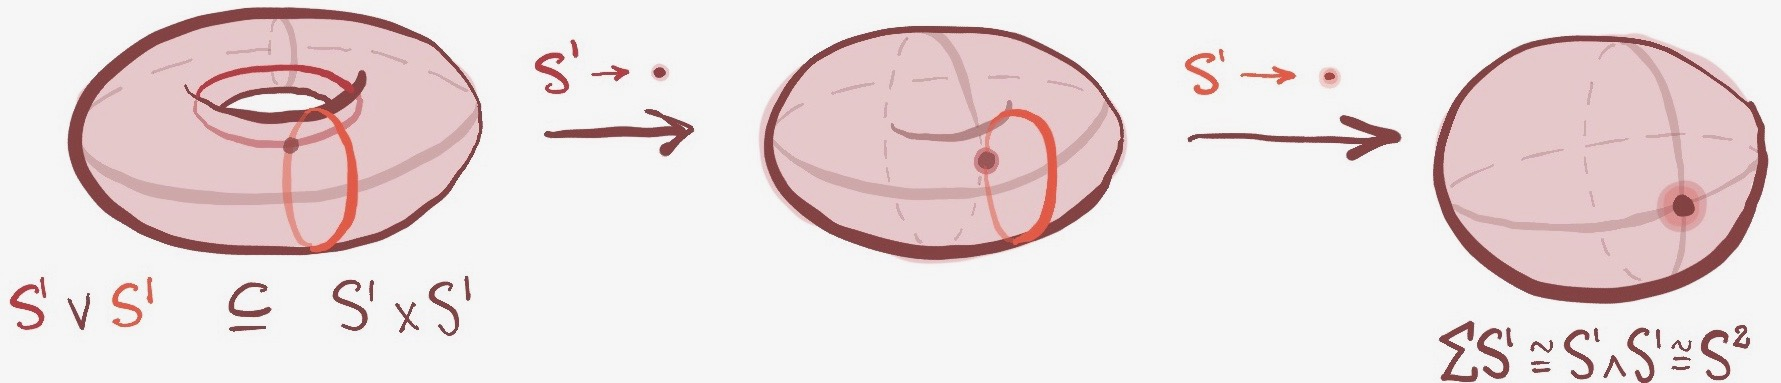
\includegraphics[width=\linewidth]{pics/s1_smash_s1.png}
  \centering
  \caption{The homeomorphism $S^1\smashprod S^1 \cong S^2$.}
  \label{fig:s1-smash-s1}
\end{figure}

In general, we have a similar homeomorphism
$$S^n \smashprod S^m \cong S^{n+m}.$$
\end{example}



Let $\Omega$ be the loop functor, which for a based space $X$ is defined as $\Omega X := \Map_\ast (S^1,X)$, i.e., the space of loops in $X$ based at the basepoint of $X$. There is an adjunction $\Sigma \adj \Omega$, which means that we have a natural homeomorphism
\begin{align*}
	\Map_\ast (\Sigma X,Y) \cong \Map_\ast (X, \Omega Y),
\end{align*}
where this homeomorphism holds in our ``convenient'' category of spaces. Alternatively this is the data of a unit $X \to \Omega \Sigma X$ and a counit $\Sigma \Omega X \to X$ satisfying certain triangle identities. From this adjunction, we will end up seeing that the set of homotopy classes of based maps are isomorphic:
\begin{align*}
	[\Sigma X, Y]_\ast \cong [X, \Omega Y]_\ast.
\end{align*}

Higher homotopy groups of a space based space $X$ are defined as homotopy classes of maps from higher dimensional spheres $\pi_n(X)=[S^n,X]_\ast$. The theorem that forms the bridge from unstable to stable homotopy theory is the \emph{Freudenthal suspension theorem}. Before stating it, we need a preliminary definition.

%This will follow from a fact that $\pi_0 (\Map_\ast (X,Y)) \cong [X,Y]_\ast$.

\begin{definition} $X$ is \textit{$n$-connected} if $\pi_i (X) = 0$ for all $i\leq n$. For example, 0-connected means path connected and 1-connected means simply connected.
\end{definition}

We may also define a suspension map on homotopy groups
\begin{align*}
	\Sigma : \pi_q (X) &\to \pi_{q+1}(\Sigma X) \\
	f &\mapsto \left[f\smashprod \id : S^{q+1} = S^q \smashprod S^1 \to X\smashprod S^1 = \Sigma X\right].
\end{align*}

\begin{theorem}\label{thm:Freudenthal-suspension} \textit{(Freudenthal suspension theorem)}
Assume that $X$ is a based space which is $n$-connected. Then the morphism $\Sigma: \pi_q(X) \to \pi_{q+1}(\Sigma X)$ is:
\begin{itemize}
	\item a bijection for $q\leq 2n$
	\item a surjection for $q= 2n+1$.
\end{itemize}
\end{theorem}

%%%% FOR LATER: n-connected map, pi_n(Z)

%\begin{definition} A map $f: X \to Y$ is \textit{$n$-connected} if the homotopy fiber is $(n-1)$-connected. Explicitly, the induced map on homotopy groups $f_\ast : \pi_i (X) \to \pi_i(Y)$ is an isomorphism for all $i<n$ and a surjection for $i=n$. This follows from the fact that homotopy fiber sequences induce a long exact sequence on homotopy groups.
%
%Another way to state this is that, for $X$ $n$-connected, the unit map of the $\Sigma$-$\Omega$ adjunction $X\to \Omega \Sigma X$ is $(2n+1)$-connected. We also note the helpful fact that
%\begin{align*}
%	\pi_i(\Omega Y) \cong \pi_{i+1}(Y),
%\end{align*}
%since $\pi_i(\Omega Y) \cong [S^i, \Omega Y]_\ast$ and $\pi_{i+1}(Y) = [S^{i+1}, Y]_\ast = [\Sigma S^i, Y]_\ast$.
%\end{definition}
%
%\begin{corollary} $\pi_n(S^n) \cong \Z$ for all $n\geq 1$.
%\end{corollary}
%\begin{proof} It will suffice to show $\pi_2(S^2)\cong \Z$, since by the Freudenthal suspension theorem this will induce isomorphisms on $\pi_n(S^n)$ for all $n\geq 2$.
%
%We may use the long exact sequence for the Hopf fibration $S^1 \hookto S^3 \xto{\eta} S^2$. Thinking of
%\begin{align*}
%	S^3 &= \{(w,z)\in \C^2 \ : \ ||(w,z)|| = 1\},
%\end{align*}
%we send $(w,z)$ to the complex line $[w:z]$ in $\C^2$. In the long exact sequence, we get
%\[
%	\begin{tikzcd}
%	\pi_2(S^1)\rar & \pi_2(S^3)\dar[equal]\rar & \pi_2(S^2) \rar["\cong"] & \pi_1(S^1)\dar[equal]\rar & \pi_1(S^3)\dar[equal]\rar & 0 \\
%	 & 0 & & \Z & 0 & \\
%	\end{tikzcd}
%\]
%
%Thus by Freudenthal suspension, we have that $\pi_n(S^n) \cong \Z$ and $\pi_n(S^n) \to \pi_{n+1}(S^{n+1})$ is an isomorphism for $n\geq 2$.
%
%For $n=1$ we need that the Hurewicz theorem commutes with suspension in homology, that is, the diagram commutes:
%\[
%	\begin{tikzcd}
%	\pi_1(S^1)\rar\dar["\Sigma" left] & H_1(S^1)\dar["\Sigma" right] \\
%	\pi_2(S^2)\rar & H_2(S^2).
%	\end{tikzcd}
%\]
%\end{proof}

By Freudenthal, $\pi_{q+n}(\Sigma^n X)$ stabilizes as $n$ increases. This stable value is an interesting invariant on the space $X$.

\begin{definition}\label{def:stable-homotopy-group} The \textit{$q$th stable homotopy group} of a space $X$ is defined to be
\begin{align*}
	\pi_q^s (X) := \colim_n \pi_{q+n}(\Sigma^n X).
\end{align*}
\end{definition}

We observe that if $X$ is $(n-1)$-connected, then for $q < n-1$, the maps in the colimit system are isomorphisms. Thus we have that $\pi_q^s(X) = \pi_{q+n}(\Sigma^n X)$ for $q < n-1$.

\begin{remark} The computations of stable homotopy groups of spheres $\pi_q^s (S^0)$ is one of the deepest problems in algebraic topology. We will observe that these groups are deeply related to many questions throughout geometry and algebra as well.
\end{remark}

We can take the idea of stabilizing a space that we have seen, and make the following definition of a \emph{spectrum}, a stable  analogue of a space.





\begin{definition} A \textit{(pre)spectrum} $X$ is a sequence of based spaces $X_0, X_1, \ldots$ equipped with structure maps
\begin{align*}
	\sigma_i : \Sigma X_i \to X_{i+1}
\end{align*}
for each $i$.
\end{definition}


\begin{example}\label{ex:sphere-spectrum} There is a \textit{sphere spectrum}, denoted $\mathbb{S}$, whose $n$th space is the $n$-sphere $S^n$. The structure maps are the homeomorphisms $S^1 \smashprod S^n \xto{\sim} S^{n+1}$ given by \autoref{ex:homeomorphism-smashing-spheres}.
\end{example}



\begin{example}\label{ex:suspension-spectrum} Given any based space $X$, we denote by $\Sigma^\infty X$ its \textit{suspension spectrum}, whose $n$th space is $\Sigma^n X$, and whose structure maps are the obvious homeomorphisms $\Sigma \Sigma^n X \xto{\sim} \Sigma^{n+1} X$. As an example, we have that $\mathbb{S} = \Sigma^\infty S^0$.
\end{example}



\begin{definition} Given a spectrum $X$, we may define the \textit{$n$th stable homotopy group of $X$} as
\begin{align*}
	\pi_n(X) &= \colim_k \left( \cdots \to \pi_{n+k}(X_k) \to \pi_{n+k+1}(\Sigma X_k) \xto{\sigma_{k,\ast}} \to \cdots \right)
\end{align*}
\end{definition}

\begin{exercise} If $X$ is a based space, then its $q$th stable homotopy group is the $q$th homotopy group of its suspension spectrum.
\end{exercise}


The collection of spectra form a category.

\begin{definition} A \textit{morphism of spectra} $X\to Y$ is a collection of maps $f_i : X_i \to Y_i$ at each level, which commute with the structure maps:
\[
	\begin{tikzcd}
	\Sigma X_i \rar["\Sigma f_i"]\dar["\sigma_i" left] & \Sigma Y_i \dar["\sigma_i" right] \\
	X_{i+1}\rar["f_{i+1}" below] & Y_{i+1}.
	\end{tikzcd}
\]
\end{definition}

Knowing what a weak homotopy equivalence of topological spaces is, we might want to define a notion of having a weak homotopy equivalence of spectra. One naive notion would be to define an equivalence to be a levelwise equivalence (i.e. $f: X \to Y$ is an equivalence if $f_i : X_i \to Y_i$ is a weak homotopy equivalence for each $i$). A better notion is to ask for a \textit{stable equivalence}.

\begin{definition} A \textit{stable equivalence} of spectra is a morphism $f: X \to Y$ so that the induced map on homotopy groups
\begin{align*}
    (f_q)_\ast : \pi_q(X) \xto{\sim} \pi_q(Y)
\end{align*}
is an isomorphism for each $q$.
\end{definition}

We may also define a category $\Ho\Sp$ which is the localization of the category of spectra at the stable equivalences. That is, a functor $\Sp \to \Ho\Sp$ which turns stable equivalences into isomorphisms, and is initial among functors with this property --- that is, if there is another functor $\Sp \to \mathscr{C}$ which sends stable equivalences to isomorphisms, we get a unique factorization
\[
	\begin{tikzcd}
	\Sp\rar\ar[dr] & \Ho\Sp\dar[dashed] \\
	 & \mathscr{C}.
	\end{tikzcd}
\]

However $\Ho\Sp$ is a difficult category to work in, since it does not have many limits or colimits.
\[
	\begin{tikzcd}
	\CW\dar\rar["\text{disjoint}" above, "\text{basept.}" below] & \CW_\ast\dar \rar["\Sigma^\infty"] & \Sp\dar & \Ab\lar["H-"above]\dar["\text{0th component}"]\\
	\Ho(\CW)\rar & \Ho(\CW_\ast)\rar & \Ho(\Sp)\rar["\pi_\ast"] & \Ab^{\Z_{\geq 0}} \\
	\end{tikzcd}
\]


For every abelian group $G$, there is an \textit{Eilenberg-Maclane spectrum} $HG$ which is described up to homotopy by the property that $\pi_0(HG) = G$ and $\pi_i(HG) = 0$ for $i\neq 0$, where $(HG)_n = K(G,n)$ for each $n$. We will construct this spectrum later on in the class.

\subsection{Why should we care about spectra?}
There is an amazing theorem called \textit{Brown representability} that states that every cohomology theory $E^\ast : \Ho\CW \to \Ab^{\Z_{\geq 0}}$, satisfying certain axioms, is represented by a spectrum $E$, that is, $E^n(X) \cong [X,E_n]$ and $E$ is unique up to isomorphism in $\Ho\Sp$. Equivalently, any spectrum yields a cohomology theory. Thus we can study generalized cohomology theories by directly studying spectra. 

Here are some questions and applications where spectra are key.

\begin{example} The enumeration of differentiable structures on spheres $S^n$ for $n\geq 5$ is reduced to the computation of the stable homotopy groups of spheres.
\end{example}
	
\begin{example} One can impose an equivalence relation on closed  manifolds called \emph{cobordism}. (Draw picture) The classification question of closed  manifolds up to cobordism is a central problem in differential topology. Amazingly, it turns out that this problem can be translated into stable homotopy theory. The groups $\Omega_n$ of closed  $n$-manifolds up to cobordism was shown by Thom to be isomorphic to the homotopy groups homotopy groups of a spectrum $\MO$.
\end{example}

\begin{example} Consider the question: \emph{For which $n$ is $\R^n$ is a division algebra?} Of course, we know four examples, $\R, \mathbb{C}=\R^2, \mathbb{H}=\R^4, \mathbb{O}=\R^8)$, are there any others? This is also equivalent to asking when $S^{n-1}$ is an $H$-space, i.e., it has a continuous multiplication map with a two-sided identity element. This question is also known as \emph{the Hopf invariant one problem} because it is also equivalent to the existence of a Hopf invariant one map $S^{2n-1}\to S^n$. This question was  solved by Adams, initially in a 100 page paper, where he introduced the Adams spectral sequence for $\pi_q^s(S^0)$. He later gave a much shorter solution using $K$-theory. Stable homotopy theory is key in both solutions.
\end{example}

\begin{example} Consider the question: \emph{How many linearly independent everywhere nonzero vector fields can there be on $S^{n-1}$?} This question was answered by Adams using $K$-theory, an extraordinary cohomology theory. The answer is that $S^{n-1}$ admits exactly $\rho(n)-1$ linearly independent everywhere nonzero vector fields, where $\rho(n)$ is the Radon-Hurwitz number equal to $2^c+8d$, where $n=(2a+1)2^b$ and $b=c+4d$ with $0\leq c<4$.
\end{example}

\begin{example} A very old question in differential topology dating back to the 1960s was: \emph{For which $n$ does there exist a stably framed $n$-manifold with the Kervaire invariant one?} This is known as the \emph{Kervaire invariant one problem}. The Kervaire invariant of a smooth stably framed manifold is the so-called Arf-invariant of an associated quadratic form $H^{\frac{n}{2}}(M, \Z/2)\to\Z/2$. The answer to the Kervaire invariant 1 problem is yes in dimensions $n=2,6,14,62$ and possibly $126$, but it was ruled out in all other dimensions in 2009 by a recent breakthrough result of Hill, Hopkins and Ravenel \cite{HHR}. This question can again be translated into the survival of certain elements in the Adams spectral sequence for the stable homotopy groups of spheres, and it was further translated by the authors into a question in equivariant stable homotopy theory and solved in that setting.
\end{example}


\section{The category of spaces}

We start with some recollections about basic category theory and we construct the ``convenient category of topological spaces" which modern algebraic topologists work in.

%%%
% LECTURE 2
% \section{Lecture 2: January 22nd}
\subsection{Category theory review}

We refer the reader to the following excellent sources for the basics of category theory. The sets of notes \cite{WOMP},\cite{Torres-cat} and \cite{mehrle} are great introductions and so are the textbooks \cite{leinster} and \cite{Riehl-context}. The standard reference for category, which was the first book on the subject is still \cite{maclane}. We skip the definition of category but recall a list of standard examples of categories that you have certainly encountered  before. 

\begin{table}[h]
    \centering
    \caption{Examples of categories}
    \begin{tabular}{ p{2cm} l  p{5cm}  p{8cm} }
        \toprule
\textbf{Category}      
& \textbf{Objects}   
& \textbf{Morphisms} \\\midrule
$\Set$ & sets & set functions \\\hline

$\Grp$ & groups &group homomorphisms \\\hline
	 $\Ab$ & abelian groups &group homomorphisms \\\hline
         $\Ring$ & rings& ring homomorphisms \\\hline
	 $\Top$& topological spaces & continuous maps\\\hline
	 $\Top_\ast$ & based spaces & based continuous maps\\\hline
	 $\Vect(k)$& vector spaces over a field $k$ & linear maps\\\hline
	 $\mathbbm{1}$ & single object & only identity arrow\\\hline
	 $\mathbbm{2}$ & two objects, denoted 0 and 1 & single non-identity morphism $0\to 1$.\\
	 \bottomrule
    \end{tabular}
\end{table}


Also, here are some examples of functors between some of these categories, which we have probably encountered before:
\begin{itemize}\itemsep0em 
	\item the {forgetful functor}\index[ind]{functor!forgetful}  $U: \Grp \to \Set$ which forgets the group structure
	\item  the {free functor}\index[ind]{functor!free} $F:\Set \to \Grp$  which takes the free group on a set
	\item  homology $H_i \colon \Top_\ast \to \Grp$ 
	\item  homotopy groups $\pi_i \colon \Top_\ast \to \Grp$ 
	\item cohomology $H^i : \Top^\ast \to \Grp$, which is a \textit{contravariant} functor.
\end{itemize}


%\begin{itemize}
%	\item $\Set$ is the category whose objects are sets and whose morphisms are functions
%	\item $\Grp$ is the category whose objects are groups and whose morphisms are group homomorphisms
%	\item $\Ab$ is the category of abelian groups
%        \item $\Ring$ is the category of rings
%	\item $\Top$ is the category whose objects are topological spaces and whose morphisms are continuous maps
%	\item $\Top_\ast$ is the category of based spaces and based continuous maps
%	\item $\Vect(k)$ is the category of vector spaces over a field $k$ whose morphisms are linear maps
%	\item $\1$ is a category with a single object and an identity arrow
%	\item $\2$ is a category with two objects, denoted 0 and 1, and a single non-identity morphism $0\to 1$.
%\end{itemize}

\begin{example} Suppose that $G$ is a group. Then we may form a category $G$ with one object, and whose morphism set is all of $G$. Composition is given by the group law. A functor $G \to \Set$ is exactly the data of a $G$-set, that is, a set equipped with an action of $G$. Similarly, a functor $G \to \C$ is referred to as a $G$-object in $\C$.
\end{example}


\begin{definition} For any category $\mathscr{C}$, we can define its \textit{opposite category}\index[ind]{category!opposite}, denoted $\mathscr{C}^\op$, whose objects are the same as $\mathscr{C}$, but whose morphisms have the domain and codomain swapped, and whose composition is defined to mirror the composition in $\mathscr{C}$. That is, a morphism $x\xto{f} y$ in $\mathscr{C}$ corresponds to a morphism $y\xto{f^\op} x$, and we define $g^\op \circ f^\op := (f\circ g)^\op$.
\end{definition}

Note that for any category $\mathscr{C}$, we have that $(\mathscr{C}^\op)^\op$ is just $\mathscr{C}$. The construction $\mathscr{C}^\op$ occurs frequently in mathematics. The opposite category $\mathscr{C}^\op$ can be very different than the category $\mathscr{C}$. Some interesting examples follow:
\vspace{-1em}
\begin{itemize}\itemsep0em 
    \item the category of affine schemes is equivalent to $\Ring^\op$
     \item the opposite category of finite sets is equivalent to the category of finite Boolean algebras
    \item the category $\Top^\op$ is, in some sense, equivalent to the category of frames  (for a discussion of this, see \cite{top-op-mathse})
\end{itemize}



{\bf Note on terminology:} The classical notion of a contravariant functor from $\mathscr{C}\to\mathscr{D}$ can be thought of as a covariant functor $\mathscr{C}^\op \to \mathscr{D}$, thus so long as we specify the domain category, we may often refer to a functor with the implicit assumption that it is covariant.



\begin{definition} Let $F,G : \C \to \D$ be covariant functors. A \textit{natural transformation}\index[ind]{natural transformation} $\eta : F \Rightarrow G$ is a collection of morphisms $\eta_x : Fx \to Gx$ for each $x\in \C$, such that, for every $x\xto{f} y$ in $\C$, we have that the diagram commutes
\[
	\begin{tikzcd}
	Fx\rar["Ff" above]\dar["\eta_x" left] & Fy\dar["\eta_y" right] \\
	Gx\rar["Gf" below] & Gy.
	\end{tikzcd}
\]
\end{definition}

\begin{definition} A \textit{natural isomorphism} is a natural transformation $\eta: F \Rightarrow G$ such that the components $\eta_c : Fc \xto{\cong} Gc$ is an isomorphism for each $c\in \C$.
\end{definition}


For any two categories $\C$ and $\D$, we can define the product category $\C\times \D$, with objects and morphisms given by pairs of objects and morphisms, and identities and composition defined componentwise. 

\begin{exercise} Show that the data of a natural transformation is the same as a functor $H : \C\times\mathbbm{2} \to \D$, such that $H(-,0)=F$ and $H(-,1) = G$. 
\end{exercise}


\begin{example} Let $(-)^{\ast\ast} : \Vect(\R) \to \Vect(\R)$ denote the double dual functor. We have a natural transformation $\eta : \id_{\Vect(\R)} \Rightarrow (-)^{\ast\ast}$ whose components are the isomorphisms $\eta_V \to V^{\ast\ast}$ given by $x\mapsto [\ev_x : V^\ast \to \R]$. One may check that the corresponding diagram commutes, and gives a natural isomorphism.
\end{example}


\begin{remark} For every $V$, there also exists an isomorphism $V\cong V^\ast$, however there is no natural isomorphism $\id \Rightarrow (-)^\ast$.
\end{remark}

\begin{definition} We define $\D^\C$ or $\Fun(\C,\D)$ as the \textit{functor category} whose objects are functors $\C\to \D$ and whose morphisms are natural transformations.\todo{Thomas: is this an okay convention though? I feel like in general, $\mathscr{D}^{\mathscr{C}}$ denotes $\mathscr{D}$-valued presheaves on $\mathscr{C}$, so functors $\mathscr{C}^\op \to \mathscr{D}$}
\end{definition}

Let $\C$ be a \textit{locally small} category, meaning that $\Hom_\C(a,b)$ is a set for each pair of objects in $\C$. For each $c\in \C$, we obtain functors
\begin{align*}
	\Hom_\C (c,-) : \C &\to \Set \\
	\Hom_\C(-,c) : \C^\op &\to \Set
\end{align*}

Functors of this form are called \emph{representable}. The Yoneda lemma says that the set of natural transformations
$\Hom_\C(-,c)\Rightarrow F$ is in bijection with $F(c)$, naturally
in $c$.
\begin{lemma}[Yoneda Lemma, covariant version] Let $F\colon \C \to \Set$. There is a bijection
\begin{align*}
	\Hom_{\Set^\C}(\Hom_\C (c,-), F) \cong F(c),
\end{align*}
naturally in both $c$ and $F$.
\end{lemma}

\begin{exercise} $\ $
Prove the Yoneda lemma.

\emph{Hint: There are two parts to this. First, define the required set isomorphism. Second, draw out the naturality squares, along maps $c\to c'$ and along natural transformations $F\Rightarrow F'$ and check that with the definition  of the isomorphism you gave, these squares commute.  A reference for the proof is for example \cite[Lemma 2.5]{mehrle}.}
\end{exercise}
There is an equivalent contravariant version of the Yoneda lemma. Moreover, it turns out we can prove two objects in a category are isomorphic by showing that the representables are naturally isomorphic.

\begin{lemma}
Suppose that there is a natural isomorphism of functors $$\eta\colon \Hom_\C(c, -)\cong \Hom_\C(d, -).$$ Then $c\cong d$ in $\C$.
\end{lemma}

\begin{proof}
We can show that $\eta_c(\id_c)\colon d\to c$ is an isomorphism. Since $\eta_d$ is an isomorphism, there exists an $f\colon c\to d$ such that $\eta_d(f)=\id_d$. Considering the naturality sqaure
\[\xymatrix{
\Hom_\C(c,c)\ar[r]^-{\eta_c}\ar[d]_-{\circ f}  & \Hom_\C(d,c) \ar[d]^-{\circ f} \\
\Hom_\C(c,d) \ar[r]_-{\eta_d}& \Hom(d,d)
}\]  we can see that $f\circ \eta_c(\id_c)\circ f=\id_d$. Similarly considering the naturality square for $\eta_c(\id_c)\colon d\to c$ we can show that $\eta_c(\id_c)\circ f=\id_c$.
\end{proof}

\subsection{Adjoint pairs of functors}

Let $\Cat$ be the category of categories and functors. Note that in any category, there is a looser way that objects can be ``the same" than equality: two objects $C$ and $D$ are defined to be isomorphic if there are morphisms $f\colon C\to D$ and $g\colon D\to C$ such that $fg=\id$ and $gf=\id$. In particular, in the category $\Cat$, two categories $\C$ and $\D$ are isomorphic if there are functors $F\colon \C\to \D$ and $G\colon \D\to \C$ such that $FG=\id$ and $GF=\id$. However, we have seen that there is a looser notion that we can use to compare functors than equality: we have defined a notion of isomorphic functors, which leads to the definition of \emph{equivalence of categories}.

\begin{definition}\label{equivcats} A functor $F\colon \C \to \D$ is an \textit{equivalence of categories} if there exists $G : \D \to \C$ such that $FG \cong \id_\D$ and $GF\cong \id_\C$ are natural isomorphisms of functors. We say that $F$ is an \textit{isomorphism of categories} if $FG = \id_\D$ and $GF = \id_\C$.
\end{definition}

Recall that for a set function having an inverse is equivalent to being injective and surjective. An analogous result regarding equivalences of categories is the following.

\begin{proposition} $F\colon \C \to \D$ is an equivalence of categories if and only if $F$ is:
\vspace{-1em}
\begin{itemize}\itemsep0em
	\item \textit{faithful}, meaning that $\Hom_\C(c,c') \hookto \Hom_\D(Fc, Fc')$ is injective for each $c,c'$
	\item \textit{full}, meaning that $\Hom_\C(c,c') \tto \Hom_\D(Fc,Fc')$ is surjective for each $c,c'$
	\item \textit{essentially surjective on objects}, meaning for each $d\in \D$ there exists $c\in \C$ such that $F(c) \cong d$.
\end{itemize}
\end{proposition}

\begin{exercise}
Prove the proposition. \emph{A reference for the proof is \cite[Proposition 1]{WOMP}.}
\end{exercise}

More generally we have a notion of having a map between functors, i.e., a natural transformation. We can ask for two categories to be related in an even weaker sense than the notion of equivalence we have defined by simply requiring that we have natural transformations between the two composites and identities, but without requiring that these are isomorphisms. We do impose a condition that ensures that the two natural transformations do interact nicely with each other.

\begin{definition}\label{def1} Given a pair of functors $F\colon \C \leftrightarrows \D:\!\! G$, we say they are \textit{adjoint} if there exist natural transformations $\eta \colon \id_\C \Rightarrow GF$ (called the \textit{unit}) and $\epsilon \colon FG \Rightarrow \id_\D$ (called the \textit{counit}) satisfying the triangle identities:

\[
	\begin{tikzcd}
	F(a)\rar["F\eta_a" above]\ar[equal, dr] & FGF(a)\dar["\epsilon_{F(a)}" right] \\
	 & F(a)
	\end{tikzcd}\quad
	\begin{tikzcd}
	G(b)\rar["\eta_{G(b)}" above]\ar[equal, dr] & GFG(b)\dar["G(\epsilon_b)" right]\\
	& G(b),
	\end{tikzcd}
\]
for each $a\in \C$, $b\in \D$.

\end{definition}

We will give three more definitions of an adjunction, which we claim are all equivalent to each other. We can define an adjunction in terms of just the unit or the counit together with a universal property.

\begin{definition}\label{def2}
Given a pair of functors $F\colon \C \leftrightarrows \D\colon G$, we say they are \textit{adjoint} if there exists a natural transformations $\eta \colon \id_\C \Rightarrow GF$ (called the \textit{unit}) such that for any object $C$ of $\C$ and $D$ of $\D$ and any map $f\colon C\to G(D)$ there exists a unique map $g \colon F(C) \to D$ so that the following diagram commutes:

\[\begin{tikzcd}
C \arrow{d}{f} \arrow{r}{\eta_C} &GF(C) \arrow[dotted]{dl}{Ug}\\
U(D)  & 
\end{tikzcd}\]
\end{definition} 

\begin{definition}\label{def3}
(Dual definition specifying the counit instead of the unit.)
\end{definition} 

Lastly, we can give a definition in terms of a natural isomorphism of hom-sets when the categories $\C$ and $\D$ are both locally small so that $\Hom_\D(F(a),b)$ and $\Hom_\C(a,G(b))$ are sets. Oftentimes, the following is given as the definition of an adjunction.

\begin{definition}\label{def4} Given a pair of functors $F: \C \leftrightarrows \D:G$, we say they are \textit{adjoint} if, for each $a\in \C$, $b\in\D$, there exists an isomorphism
\begin{align*}
	\Hom_\D(F(a), b) \cong \Hom_\C (a, G(b)),
\end{align*}
which is natural in both $a$ and $b$.
\end{definition}

\begin{exercise} Demonstrate the equivalence of these four definitions. 
\end{exercise}

Hint: These equivalences of definitions can all be found in the nLab entry on adjunctions. Also, the proof of the equivalence of \autoref{def1} and \autoref{def4} can be found as  \cite[Theorem 2.2.5]{leinster} or \cite[Theorem 3.9]{mehrle}. The equivalence of \autoref{def2} and \autoref{def4} can be found in \cite[Section 3]{henderson} or \cite[Theorem 2.3.6.]{leinster}, where the universal property of the unit is formulated in terms of initial objects. The argument using \autoref{def3} instead of \autoref{def2} should be exactly analogous.

%\warning The second definition only makes sense in a setting where we are allowed to compare $\Hom_\D(F(a),b)$ and $\Hom_\C(a,G(b))$, for example when $\C$ and $\D$ are both locally small.


\begin{examples}\label{exs:adjunctions} Here are some examples of adjunctions:
\begin{itemize}
	\item Fix an abelian group $B$. Then for any abelian groups $A$ and $C$, we have a natural isomorphism of sets
\begin{align*}
	\Hom_\Ab (A\otimes B, C) \cong \Hom_\C(A, \Hom_\Ab (B,C)).
\end{align*}
That is, the functors $-\otimes B$ and $\Hom_\Ab (B, -)$ are adjoint.
	\item We have an free-forgetful adjunction $F: \Set \leftrightarrows \Grp : U$
	\item $(-)_+ : \Top \leftrightarrows \Top_\ast: U$ is an adjunction. We see this since
	\begin{align*}
		\Top(X,UY) \cong \Top_\ast (X_+, Y).
	\end{align*}
\end{itemize}
\end{examples}



\begin{proposition} Adjoints compose.
\end{proposition}

\begin{exercise}\label{exer:left-adjoint-fully-faithful-iff-unit-natural-iso}
Let $F : \mathscr{C} \rightleftarrows \mathscr{D} : G$ be an adjunction. Then
\begin{enumerate}
    \item $F$ is fully faithful if and only if the unit $\eta: \id_\mathscr{C} \to GF$ is a natural isomorphism.
    \item $G$ is fully faithful if and only if the counit $\epsilon : FG \to \id_\mathscr{D}$ is a natural isomorphism.
\end{enumerate}

\end{exercise}



Note that in \autoref{equivcats} of equivalence of categories we only required that $GF\cong\id $ and $FG\cong \id$ were natural isomorphisms, but not necessarily that $F$ and $G$ are adjoint (namely, the triangle identities were not imposed). It turns out that every equivalence of categories can be modified to an adjoint equivalence by possible changing the unit or counit. For a proof, see \cite[Lemma 3.10]{mehrle}.


\subsection{A convenient category of spaces}

\epigraph{For many years, algebraic topologists have been laboring under the handicap of not knowing in which category of spaces they should work. Our need is to be able to make a variety of constructions and to know that the results have good properties without the tedious spelling out at each step of lengthy hypotheses such as countably paracompact, normal, completely regular, first axiom of countability, metrizable, and so forth. It may be good research technique and an enjoyable exercise to analyse the precise circumstances for which an argument works; but if a developing theory is to be handy for research workers and attractive to students, then the simplicity of the fundamentals must be the goal.}{\cite{Steenrod-convenient-cat}}

The main references for this section are \cite{Steenrod-convenient-cat} and \cite{Strickland-cgwh}, and we refer the reader to those papers for all of the proofs of point set topology propositions. An excellent set of notes on this topic is also \cite{martincgwh}.

Recall that in $\Set$ we have an adjuction between the product and the hom functor given by 
$$\Hom_\Set(A\times B, C)\cong \Hom_\Set (A, \Hom_\Set(B,C)).$$ Of course, the bijection follows from comparing cardinalities, but the point is that these bijections are natural, so they are compatible along morphisms in the category. We want a similar adjunction in the category of spaces. 

Let $Y^X$ or $\Map(X,Y)$ denote the \textit{mapping space} between two topological spaces, whose underlying set is the collection of continuous maps $X\to Y$, and which is equipped with the \textit{compact-open topology}, generated by the subbasis
\begin{align*}
	W_{K,U} = \{ f: X \to Y \ : \ f(K)\subseteq U\},
\end{align*}
indexed over $K\subseteq X$ compact and $U\subseteq Y$ open. We have a map
\begin{align}\label{eqn:mapping-space-adjunction}
	\Map(X\times Y, Z) \to \Map (X, \Map(Y,Z)),
\end{align}
which is always a homeomorphism onto its image, but it is not always surjective. Thus $\Map(Y,-)$ and $-\times Y$ are not adjoint. As we will see in the next section, any left adjoint in $\Top$ would need to preserve quotients, which is a type of colimit. However, by \cite[Section 22, Example 7]{munkres}, The product of the quotient map  $\R\to \R/\sim$, which identifies all of $\N$ to a point, with $\Q$ is not a quotient. Thus $- \times \Q$ cannot possibly be a left adjoint.

In order to turn Equation \ref{eqn:mapping-space-adjunction} into a homeomorphism,
%%%
% LECTURE 3
% \section{Lecture 3: January 24th}
we define a class of spaces for which this is a homeomorphism. %One idea would be to modify the definition of the compact-open topology to a subbasis using $K$ which are images of arbitrary compact Hausdorff spaces.

\begin{definition} A subspace $A\subseteq X$ is \textit{$k$-closed in $X$} if, for all compact Hausdorff spaces $K$ and continuous maps $K \xto{f} X$, we have that $f^{-1}(A)$ is closed in $K$.\index[ind]{$k$-closed}
\end{definition}

\begin{exercise} The collection of $k$-closed subsets of $X$ forms a topology which contains the original topology on $X$ (since closed implies $k$-closed).
\end{exercise}

Let $kX$ denote the set $X$ equipped with the $k$-closed topology. So $kX$ has the same underlying set as $X$ but its topology has more closed sets. We note that the identity map $kX \to X$ is continuous.

\begin{definition} We say that a space $X$ is \textit{compactly generated (CG)} if the identity map $kX \to X$ is a homeomorphism. That is, if every $k$-closed set is closed in the original topology on $X$.\index[ind]{compactly generated}
\end{definition}

Some examples of CG spaces are metric spaces and all locally compact spaces, so in particular, CW complexes. The proofs that these spaces are CG can be found in \cite[Propositions 1.6, 1.7]{Strickland-cgwh}


Note that immediately from the definitions, if $X$ is a compactly generated space, and $Y$ is any space, then $f: X \to Y$ is continuous if and only if $f: X \to kY$ is continuous. 

\begin{upshot} For the functors $i:\CG \leftrightarrows \Top:k$, we have that
\[
	\Hom_\Top (iX,Y) \cong \Hom_\CG (X, kY),
\]
so $i$ is left adjoint to $k$.

\end{upshot}



\begin{note} We have that $k^2 X = kX$.
\end{note}

\begin{note} The category $\CG$ is not closed under product and mapping spaces. So we must define
\begin{align*}
	X\times_k Y &:= k(X\times Y) \\
	\Map_k (X,Y) &:= k\Map(X,Y).
\end{align*}
\end{note}

\begin{theorem} There exists a homeomorphism
\begin{align*}
	\Map(X\times_k Y, Z) \cong \Map_k (X, \Map_k (Y,Z)),
\end{align*}
so $\CG$ is Cartesian closed. For a proof of this theorem, read \cite[Proposition 2.11]{Strickland-cgwh}.
\end{theorem}

The category $\CG$ is good enough for most applications, but to make things a little better, we impose an additional separation axiom.

\begin{definition} A topological space is \textit{weak Hausdorff}\index[ind]{weak Hausdorff} if for all compact Hausdorff spaces $K$ and every continuous map $f: K \to X$, we have that $f(K)$ is closed in $X$.
\end{definition}

\begin{exercise} Hausdorff implies weak Hausdorff.
\end{exercise}

Some examples of weak Hausdorff spaces are again CW complexes, metric spaces, etc. One of the reasons why we work with weak Hausdorff spaces as opposed to Hausdorff spaces is for example, for any closed inclusion $A\hookrightarrow X$ where $X$ is weak Hausdorff, the quotient is also weak Hausdorff, though this would not necessarily be true in Hausdorff spaces.  For example, the quotient of the $C_2$-action on a pair of real lines $\R$ which swaps the points between the lines outside of 0, and fixes $0$ on both lines is the ``line with two origins," which is not Haurdorff. Another example is the quotient of the action of the additive subgroup $\Q$ on $\R$, which is $\R/\Q$, which has the trivial topology so it is not Hausdorff.

\begin{proposition} For a weak Hausdorff space $X$, any larger topology on $X$ (i.e. a topology containing the original topology on $X$) will also be weak Hausdorff.
\end{proposition}

Another reason why we like weak Hausdorff spaces is because they interact nicely with compactly generated spaces. For example, by \cite[Lemma 1.4. and Proposition 2.14]{Strickland-cgwh}
\vspace{-1em}
\begin{itemize}\itemsep=0em
\item for $X$ is a $k$-space, it is weak Hausdorff if and only if the diagonal $X\xrightarrow{\Delta} X\times_k X$ is closed,
\item for $X$ weak Hausdorff, it is a $k$-space if and only if the closed set $C$ are precisely those for which $C\cap K$ is closed for every compact Hausdorff $K\subseteq X.$
\end{itemize}

\begin{proposition} For $X \in \CG$, we have that $X\Big/\sim$ is weak Hausdorff for some equivalence class on $X$ if and only if $\sim$ is closed (meaning the equivalence relation is closed as a subspace of $X\times X$).
\end{proposition}

For the proof of this, read \cite[Corollary 2.21]{Strickland-cgwh}. Now, by \cite[Proposition 2.22]{Strickland-cgwh}, there is a smallest closed equivalence relation on a CG space $X$, so we can make the following definition.

\begin{definition} For $X\in \CG$, let $hX = X\Big/\sim$, where $\sim$ is the smallest closed equivalence relation on $X$. Let $j: \CGWH \to \CG$ denote the inclusion. Thus we have an adjunction
\begin{align*}
	h : \CG \leftrightarrows \CGWH: j.
\end{align*}
That is, $\Hom_\CG (X, jY) \cong \Hom_\CGWH (hX,Y)$. % TODO: is h a localization of model cats? what morphisms is it inverting? is it the morphisms $X \to X\Big/\sim$?
\end{definition}

\begin{proposition} If $X,Y\in \CGWH$ then $\Map_k (X, Y)$ and $X\times_k Y$ are in $\CGWH$. So $\CGWH$ is cartesian closed.
\end{proposition}

In other words, once in $\CG$, passing to weak Hausdorff spaces, does not change products and mapping spaces. For the proofs, again see \cite[Corollary 2.16 and Proposition 2.24]{Strickland-cgwh}.

\subsection{Limits and colimits in categories}

\begin{definition} Let $F: I\to \C$ be a functor. We call this an \textit{$I$-shaped diagram in $\C$}. The \textit{colimit}\index[ind]{colimit} of $F$, denoted $\colim F$, is an object in $\C$ together with a family of morphisms $F(X) \to \colim F$ for each $X \in I$, such that
\[
	\begin{tikzcd}
	F(X)\ar[dr] \ar[rr] & & F(Y)\ar[dl] \\
	 & \colim F &
	\end{tikzcd}
\]
commutes for each $X\to Y$ in $I$, and moreover it satisfies a universal property so that for any other object $A\in\C$ with the above properties, we have that there exists a unique map $\colim F \to A$ such that the diagram commutes
\[
	\begin{tikzcd}
	F(X)\ar[dr]\ar[ddr,bend right=10] \ar[rr] & & F(Y)\ar[dl]\ar[ddl,bend left=10] \\
	 & \colim F\dar[dashed] & \\
	 & A &
	\end{tikzcd}
\]
for each $X\to Y$.
\end{definition}

The \textit{limit} of a diagram $F: I \to \C$ is dual to this definition, meaning that a limit is a colimit in the opposite category $\C^\op$, i.e. the colimit of the composite functor $I\xto{F} \C \to \C^\op$.\index[ind]{limit}

\begin{proposition}\label{prop:limits-unique-up-to-iso} Limits and colimits, when they exist, are unique up to isomorphism.
\end{proposition}

\begin{exercise}
Prove \autoref{prop:limits-unique-up-to-iso}.
\end{exercise}

Before moving on to many examples, we state a proposition whose usefulness is hard to overestimate. It says that left adjoints preserve colimits and right adjoints preserve limits.

\begin{proposition}\label{prop:LAPC} (\textit{LAPC and RAPL}\footnote{Left adjoints preserve colimits and right adjoints preserve limits.}) Let $F\adj G$ be adjoint functors. Then $F$ preserves colimits and $G$ preserves limits.
\end{proposition}

\begin{exercise}
Prove \autoref{prop:LAPC}.

 Hint: Note that if you prove that right adjoint preserve limits, it will dually follow that left adjoints preserve colimits by considering opposite categories. Now, to prove RAPL, the simplest way to approach it is straight from the hom bijection definition of adjoints and the definition of limit. Namely, show that if $L$ is a limit of a diagram in the domain category $\C$ then $GL$ satisfies the universal property of the limit in the target category $\D$. Another way would be to show that the proposition holds for representables and then go from there. Or, we using \autoref{diagonallimit}, which we will see in the next section, assuming limits exist, you can use that adjunction to prove that a right adjoint preserves limits.
\end{exercise}


\begin{definition} Let $I = \dot \ \  \dot$ be the discrete category with two objects and no nontrivial morphisms. Then the limit over $I$ is called the \textit{product}, and the colimit over $I$ is called the \textit{coproduct}.\index[ind]{product}\index[ind]{coproduct} Explicitly, where 0 and 1 denote the two objects in $I$, we have that
\begin{align*}
	\lim_I F = F(0) \Pi  F(1) \\
	\colim_I F = F(0) \amalg F(1).
\end{align*}
\end{definition}

\begin{examples} What follows are some examples of products and coproducts:
\begin{itemize}\itemsep0em
	\item In $\Set$, a functor determines two sets $F(0) = A$ and $F(1) = B$, and their colimit $A\amalg B$ satisfies the universal property that, for any other set $X$ equipped with morphisms $A\to X$ and $B\to X$, there is a unique map $A \amalg B \to X$ such that
\[
	\begin{tikzcd}
	A\ar[dr]\ar[ddr,bend right=10] & & B\ar[dl]\ar[ddl,bend left=10] \\
	 & A \amalg B\dar[dashed] & \\
	 & X &
	\end{tikzcd}
\]
commutes. This is exactly the coproduct of sets that we are familiar with. Dually, the limit $A\prod B$ satisfies the dual property that, for any $X$ equipped with maps $X\to A$ and $X\to B$, there is a unique map such that
\[
	\begin{tikzcd}
	& X\ar[ddr,bend left=10]\ar[ddl,bend right=10]\dar[dashed] & \\
	& A \prod B\ar[dl]\ar[dr] & \\
	 A & & B. \\
	\end{tikzcd}
\]
Thus the product in $\Set$ is just the cartesian product.

	\item In $\Top$, the coproduct is disjoint union and the product is the product of spaces with the product topology.

	\item In $\Top_\ast$, the coproduct is the wedge $A \vee B$, and the product is just the product of spaces $(A,a_0)\times (B,b_0)$ based at the point $(a_0, b_0)$.

	\item In $\Poset$, the product $p\smashprod q$ is the greatest lower bound, and the coproduct $p\vee q$ is the least upper bound (if they exist).

	\item In $\Grp$, the product is the direct product, and the coproduct is the free product of groups.

%	\item In $\CG$, the product is $\times_k$.
\end{itemize}
\end{examples}


\begin{definition} If $I = \dot \rightrightarrows \dot$, then the colimit over $I$ is called the \textit{coequalizer} and the limit over $I$ is called the \textit{equalizer}.\index[ind]{equalizer}\index[ind]{coequalizer}
\end{definition}

\begin{example} In $\Top$, let $E\subseteq X\times X$ be an equivalence relation on $X$. Then
	\begin{align*}
		\colim \left( E \underset{\pi_2}{\overset{\pi_1}{\rightrightarrows}} X \right) = X\big/\sim.
	\end{align*}
\end{example}

\begin{definition} If $I = \dot \from \dot \to \dot$, then the colimit over $I$ is called the \textit{pushout}.\index[ind]{pushout} The limit over $I^\op = \dot \to \dot \from \dot$ is called the \textit{pullback}.\index[ind]{pullback} We denote these by
\[
	\begin{tikzcd}
	Z\dar\rar & Y\dar \\
	X\rar & X\amalg_Z Y\po
	\end{tikzcd}\quad\quad
	\begin{tikzcd}
	X\times_Z Y \pb\rar\dar & Y\dar \\
	X\rar & Z.
	\end{tikzcd}
\]
\end{definition}

\begin{examples} Here are some examples of pushouts:
\begin{itemize}\itemsep0em
    \item In $\Set$, the pushout
	\[
		\begin{tikzcd}
			Z\dar["g" left]\rar["f" above] & Y\dar["i_2" right] \\
			X\rar["i_1" below] & X\amalg_Z Y \po
		\end{tikzcd}
	\]
	is given by $X\amalg_Z Y = (X\amalg Y)\Big/(i_1 f(z) \sim i_2 g(z))$.

	If $X,Y\subseteq S$ are both subsets of some larger set with $X\cap Y = Z$, then the pushout is $X\cup Y$.
	\item In $\Top$ the pushout is a gluing construction
	\[
		\begin{tikzcd}
		Z\dar[hook]\rar["f"] & Y\dar \\
		X\rar & X\cup_Z Y\po,
		\end{tikzcd}
	\]
	where $Z\to X$ is some nice map like a closed inclusion, then we have that
	\begin{align*}
		X\cup_f Y = X\cup_f Y = X\amalg Y \Big/ f(z) \sim z.
	\end{align*}

	For example, given the boundary inclusion $S^1 \to D^2$, we have that
	\[
		\begin{tikzcd}
		S^1\dar[hook]\rar[hook] & D^2\dar \\
		D^2\rar & S^2. \po
		\end{tikzcd}
	\]

	\item In $\Set$, the pullback
	\[
		\begin{tikzcd}
		X\times_Z Y\rar\dar\pb & Y\dar \\
		X\rar & Z
		\end{tikzcd}
	\]
	is given by
	\begin{align*}
		X\times_Z Y := \{(x,y)\in X\times Y \ : \ f(x) = g(y)\}.
	\end{align*}

	For example, given the parity map $\Z\to \Z\big/2$, the pullback along the trivial map from 0 is:
	\[
		\begin{tikzcd}
		2\Z\rar\dar\pb & \Z\dar \\
		0\rar & \Z\big/2.
		\end{tikzcd}
	\]

	More generally, given $f: X\to A$, the pullback of $f$ along the inclusion $\ast \to A$ which picks out a point $a\in A$ is given by:
	\[
		\begin{tikzcd}
		f^{-1}(a) \rar\dar\pb & A\dar["f" right] \\
		\ast\rar["a" below] & X
		\end{tikzcd}
	\]
\end{itemize}
\end{examples}




\begin{example} Recall that a CW complex $X$ has a discrete set $X_0$ and has skeleta $X_{n+1}$ which is built from $X_n$ via a pushout diagram
\[
	\begin{tikzcd}
	\coprod_\alpha S^n \dar["\amalg_\alpha f_\alpha" left]\rar & \coprod_\alpha D^{n+1}\dar \\
	X_n\rar & X_{n+1} \po.
	\end{tikzcd}
\]
where $\amalg_\alpha f_\alpha$ are the attaching maps. Then we define
\begin{align*}
	X = \bigcup_n X_n = \colim \left( X_0 \to X_1 \to \cdots \right)
\end{align*}
with the \textit{weak topology}, meaning that $A\subseteq X$ is closed if and only if $A\cap X_n$ is closed for each $n$.\index[ind]{weak topology}
\end{example}

%%%
% LECTURE 4
% \section{Lecture 4: January 29th}

\begin{proposition} CW complexes are in $\CGWH$.
\end{proposition}

\begin{note} The product of CW complexes $X\times Y$ gets a cell structure with $n$-cells of $X\times Y$ corresponding to a $p$-cell of $X$ and a $q$-cell of $Y$ where $p+q=n$. The idea behind this is that
\[
    D^{p+q} \cong I^{p+q} \cong I^p \times I^q \cong D^p \times D^q.
\]
\end{note}

The issue is that the product of two CW complexes $X\times Y$ is only a CW complex if the product topology is the same as the weak topology. We also note that the product topology is generally not as fine as the weak topology.


There were some partial results known before the introduction of CGWH spaces.
\vspace{-1em}
\begin{enumerate}\itemsep0em
	\item Whitehead '49 showed that if $X$ and $Y$ are CW complexes, and one is locally finite, then $X\times Y$ is CW\todo{citation sneeded}
	\item Milnor '56 showed that if both are locally countable, then $X\times Y$ is CW
	\item Tanaka '82 counterexample: if $X$ and $Y$ are CW and neither are locally countable, then $X\times Y$ is \textit{not} CW.
\end{enumerate}



But the good news is that in $\CGWH$ we have that $X\times_k Y$ is always a CW complex. A proof can be found in \cite[Theorem A.6]{Hatcher}.

\subsection{Existence of limits and colimits in $\Top$}

\begin{definition} A category with all limits is called \textit{complete}, and a category with all colimits is called \textit{cocomplete}.\index[ind]{category!(co)complete}
\end{definition}

We start with a remark about a way to describe limits when they exist. 

\begin{remark}\label{diagonallimit} We may check that, in any $\C$ which has $J$-shaped limits,
	\begin{align*}
		\Hom_\C (Z, \lim_J F) \cong \Hom_{\C^J} (\Delta  Z, F)
	\end{align*}
	where $\Delta : \C \to \C^J$ is the diagonal functor which sends $c$ to the constant diagram at $c$.
\end{remark}

\begin{proposition} If $\C$ has arbitrary coproducts and coequalizers, then it is cocomplete. Dually, if $\C$ has arbitrary products and equalizers, then it is complete.
\end{proposition}

\begin{proposition} $\Top$ is complete and cocomplete.
\end{proposition}
\begin{proof}[Proof idea] Note that we have coproducts given by disjoint union, and coequalizers are given by quotients
\begin{align*}
	\coeq \left( X \overset{f}{\underset{g}{\rightrightarrows}} Y \right) := X\Big/f(x) \sim g(x).
\end{align*}
Products are given by products, and we may check that equalizers are a subspace given by equality of two functions.

\end{proof}

\begin{proposition} The category $\CGWH$ is  complete and cocomplete.
\end{proposition}

\begin{proof}

Recall that we had adjunctions
\begin{align*}
	\Top \overset{k}{\underset{i}{\rightleftarrows}} \CG \overset{j}{\underset{h}{\leftrightarrows}} \CGWH,
\end{align*}
where the right adjoints are displayed on top.

\begin{enumerate}
	\item We have that $i$ preserves colimits, so colimits of CG spaces are computed in $\Top$ when they exist. So we must check that coequalizers and coproducts of CG spaces are CG (exercise).

	For limits, we claim that $\displaystyle \lim_J D$ for $D\colon J\to \CG$ is $\displaystyle k\lim_J (i\circ G)$ in $\CG$.
First note that
	\begin{align*}
		\Hom_\CG (X, k\lim_J (i\circ D)) \cong \Hom_\Top (iX, \lim_J (i \circ D)).
	\end{align*}
	
	Using \autoref{diagonallimit}, we have that
	\begin{align*}
		\Hom_\Top (iX, \lim_J( i \circ D)) &\cong \Hom_{\Top^J} (\Delta(iX), iD) \\
		&\cong \Hom_{\Top^J} (i\circ \Delta X, iD) \\
		&\cong \Hom_{\CG^J} (\Delta X, k\circ iD) \\
		&\cong \Hom_{\CG^J}(\Delta X, D),
	\end{align*}
	where this last isomorphism is since $D$ already takes values in $\CG$. Finally, we see that
	\begin{align*}
		\Hom_{\CG^J}(\Delta X, D) &\cong \Hom_\CG (X, \lim_J D).
	\end{align*}

	Since this is true for all objects $X$, we may check that $k\lim_J (i\circ D) = \lim_J D$.


	\textbf{Upshot}: We have that $\CG$ is complete and cocomplete and we know how to compute limits and colimits:
	\begin{itemize}
		\item colimits: do nothing except compute them in $\Top$
		\item limits: just apply $k(-)$ to it.
	\end{itemize}

	\item Since $j$ preserves limits, we have that $\CGWH$ is complete if all limits of $\CG$ spaces exist in $\CGWH$. We must check this on products and equalizers (exercise). For colimits, we need to apply $h$ to the colimit in $\CG$, similarly to as we did above.
\end{enumerate}

So we have that $\CGWH$ is complete, cocomplete, and cartesian closed.
\end{proof}

\begin{notation} From here on we redefine the category of topological spaces to be $\Top := \CGWH$, and redefine $\times := \times_k$, $\Map := k\Map$. 
\end{notation}

\subsection{The category of based topological spaces}
Let $\Top_\ast$ be the category of based (CGWH) spaces and based maps. Let $\Map_\ast (X, Y)$ be the space of based maps, and  note that we may base this mapping space at the constant map sending every $x\in X$ to the basepoint $y_0$ of $Y$.

The functor $\Map_\ast (X, -)$ has an adjoint, but it is not given by the product! Instead, the functor $X\smashprod -$ is an adjoint. We can verify that, for any other based spaces $Y$ and $Z$ we have a natural isomorphism
\begin{align*}
	\Hom_{\Top_\ast} (Y\smashprod X, Z) \cong \Hom_{\Top_\ast} (Y, \Map_\ast (X,Z)).
\end{align*}

\begin{lemma} There exist natural isomorphisms
\begin{enumerate}
	\item $(X\smashprod Y) \smashprod Z \cong X\smashprod (Y\smashprod Z)$
	\item $X\smashprod Y \cong Y\smashprod X$
	\item $X\smashprod S^0 \cong X \cong S^0 \smashprod X$.
\end{enumerate}
\end{lemma}

\begin{proof}[Proof idea] For (1), it is important that we are in $\CGWH$. By \cite[Proposition 2.20]{Strickland-cgwh}, products preserve quotients, so that 
\begin{align*}
	X\times Y \times Z \to (X\smashprod Y)\times Z \to (X\smashprod Y)\smashprod Z.
\end{align*}
is a composite of quotient maps, and may be identified with the quotient
\begin{align*}
	X\times Y \times Z \to \frac{X\times Y\times Z}{X\vee Y\vee Z}.
\end{align*}
Thus it does not depend on the order.

\end{proof}

We remark that the associativity isomorphism does not hold in the category of all topological spaces. A counterexample is given by $(\N\smashprod \Q)\smashprod \Q)$ which is not homeomorphic to $\N\smashprod (\Q \smashprod \Q)$. For a discussion see this \href{https://mathoverflow.net/questions/196084/counterexample-for-associativity-of-smash-product}{mathoverflow post}.




\begin{definition} A \textit{symmetric monoidal category}\index[ind]{symmetric monoidal category} is a triple $(\C,\otimes,\mathbbm{1})$, where $\mathscr{C}$ is a category, $\mathbbm{1}\in \mathscr{C}$ is an object, and $\otimes$ is a bifunctor
\begin{align*}
	- \otimes - : \C \times \C \to \C,
\end{align*}
such that there are natural isomorphisms
\begin{align*}
	(c\otimes d)\otimes e &\cong c\otimes (d\otimes e) \\
	c\otimes d & \cong d\otimes c \\
	\mathbbm{1} \otimes c &\cong c \cong c\otimes \mathbbm{1},
\end{align*}
for any objects in $\C$, such that all possible diagrams involving these commute (infinite data, really hard to check). However by MacLane's coherence theorem, we only need to check a few diagrams (in particular, the pentagon), and it then follows that all higher diagrams commute.
\end{definition}

\begin{definition} A symmetric monoidal category is \textit{closed}\index[ind]{symmetric monoidal category!closed} if $-\otimes X$ has an adjoint for all $X$.
\end{definition}

\begin{proposition} $(\Top_\ast, \smashprod, S^0)$ is a closed symmetric monoidal category.
\end{proposition}


\section{Higher homotopy groups}
\subsection{Homotopies}
Recall for $f,g : X \to Y$, a \textit{homotopy}\index[ind]{homotopy} $h$ from $f$ to $g$ is a map
\begin{align*}
	h : X\times I \to Y
\end{align*}
such that $h(x,0) = f(x)$, and $h(x,1) = g(x)$ for all $x\in X$. We write $f\simeq g$ to denote the homotopy.

\begin{definition} Let $[X,Y]$ be the set of homotopy equivalence classes of maps $X\to Y$ (check that $\simeq$ gives an equivalence relation).
\end{definition}

\begin{proposition} Let $X,Y \in \Top$. Then there is a bijection
\begin{align*}
	[X,Y] \xto{\cong} \pi_0 \Map(X,Y).
\end{align*}
\end{proposition}
\begin{proof} We note that
\begin{align*}
	\Map(I\times X, Y) \cong \Map(I, \Map(X,Y)),
\end{align*}
so a homotopy $f\simeq g$ corresponds to a path between $f$ and $g$ in the mapping space $\Map(X,Y)$.
\end{proof}

\begin{definition}\label{def:based-homotopy} A \textit{based homotopy}\index[ind]{homotopy!based} from $f$ to $g$, where $f,g : (X,x_0) \to (Y,y_0)$ is a homotopy $h:f\simeq g$ with the extra condition that each $h(-,t) : (X,x_0) \to (Y,y_0)$ is based.

We should check that this is equivalent to a based map $h : X \smashprod I_+ \to Y$.
\end{definition}

\begin{notation} The set of based homotopy equivalence classes of maps is denoted $[X,Y]_\ast$. For example, $[S^1, (X,x_0)]_\ast = \pi_1(X,x_0)$.
\end{notation}

\begin{definition} We say that two spaces are \textit{homotopy equivalent} if there exist maps $f: X \to Y$ and $g : Y \to X$ such that $f\circ g\simeq \id_Y$ and $g\circ f \simeq \id_X$.
\end{definition}

\begin{exercise} Show that $\simeq$ is an equivalence relation on objects in $\Top$.
\end{exercise}

\begin{proposition} Homotopy equivalence satisfies ``2 out of 3'': meaning if two out of the maps $f, g, g\circ f$ are homotopy equivalences, then so is the third (check).

\[
	\begin{tikzcd}
	X\rar["f"]\ar[dr,"g\circ f" below left] & Y\dar["g" right] \\
	 & Z.
	\end{tikzcd}
\]

\begin{note} The property ``2 out of 3'' holds automatically for all categorical isomorphisms.\footnote{In fact, the class of isomorphisms satisfies a stronger property, called \textit{2-out-of-6}.}
\end{note}

\end{proposition}

\begin{definition} A space $X$ is \textit{contractible}\index[ind]{contractible} if it is homotopy equivalent to a point (e.g. $I$, $D^n$, $\R^n$, $S^\infty$, ...).
\end{definition}

\begin{definition} The \textit{cone}\index[ind]{cone} on $X$ is defined to be the quotient space $CX := \frac{X\times I}{X\times \{1\}}$.
\end{definition}


\begin{exercise} $\ $
\begin{enumerate}
	\item Show $X$ is contractible if and only if $\id_X$ is null-homotopic (homotopic to a constant map)
	\item Show that $f: S^n \to Y$ is null-homotopic if and only if there exists an extension of $f$ to the closed disk
	\[
		\begin{tikzcd}
		S^n\rar["f"]\dar[hook] & Y \\
		D^{n+1}\ar[ur,dashed,"\widetilde{f}" below right] &
		\end{tikzcd}
	\]

	\item More generally, show that $f: X \to Y$ is null-homotopic if and only if there exists an extension
	\[
		\begin{tikzcd}
		X\rar["f"]\dar[hook] & Y \\
		CX\ar[ur,dashed,"\widetilde{f}" below right] &
		\end{tikzcd}
	\]
\end{enumerate}
\end{exercise}



%%%
% LECTURE 5
% \section{Lecture 5: January 31st}

\begin{definition} The \textit{homotopy category of $\Top$},\index[ind]{homotopy category!of $\Top$} denoted $\Ho(\Top)$, is the category whose objects are topological spaces, and whose morphisms are given by
\begin{align*}
	\Hom_{\Ho(\Top)} (X,Y) = [X,Y].
\end{align*}
An isomorphism in $\Ho(\Top)$ is the equivalence class of a homotopy equivalence $X\to Y$.
\end{definition}

There exists an obvious functor $\Top \xto{\gamma} \Ho(\Top)$ sending a map to its equivalence class.

\begin{proposition} The functor $\gamma : \Top \to \Ho(\Top)$ is universal among functors $F: \Top \to \C$ which send homotopy equivalences into isomorphisms. \footnote{This is equivalent to being homotopy invariant, meaning $F(f) = F(g)$ if $f\simeq g$.} 
That is, for any such functor, it factors uniquely as
\[
	\begin{tikzcd}
	\Top\dar["\gamma" left]\rar["F" above] & \C \\
	\Ho(\Top)\ar[ur,dashed,"\exists!" below right] &
	\end{tikzcd}
\]
\end{proposition}
\begin{proof} We will define $\phi_F : \Ho(\Top) \to \C$ on objects to be $\phi_F(X) = F(X)$. For a morphism $\alpha : X \to Y$ in $\Ho(\Top)$, let $f_\alpha : X\to Y$ be a representative of $\alpha$ in $\Top$. Then we define $\phi_F (\alpha) = F(f_\alpha)$.

To see that this is well-defined, suppose $g\simeq f_\alpha$. Then there exists $h\colon X\times I \to Y$ such that $h \circ i_0 = f_\alpha$ and $h \circ i_1 = g$, where $i_0,i_1 \colon X \to X\times I$ are the inclusions at time 0 and 1. Let $\pi_X \colon X\times I \to X$ be the projection on $X$, and note that $i_0, i_1, \pi_X$ are all homotopy equivalences. Therefore $F(i_0), F(i_1), F(\pi_X)$ are all isomorphisms. We note also that
\begin{align*}
	\pi_X \circ i_0 = \id_X = \pi_X \circ i_1.
\end{align*}
Thus
\begin{align*}
	F(\pi_X) \circ F(i_0) = \id_{F(X)} = F(\pi_X) \circ F(i_1).
\end{align*}
Since $F(\pi_X)$ is an isomorphism, we cancel it to see $F(i_0) = F(i_1)$. Then
\begin{align*}
	F(g) &= F(h) \circ F(i_1) = F(h)\circ F(i_0) = F(f_\alpha).
\end{align*}

Thus $\phi_F$ is well-defined, and we may check that it is a functor, and that it is unique (exercise).
\end{proof}

Similarly, we may define $\Ho(\Top_\ast)$ whose objects are based spaces, and whose morphisms are given by
\begin{align*}
	\Hom_{\Ho(\Top_\ast)} = [X,Y]_\ast,
\end{align*}
which are the classes of based maps under based homotopy. We note that $[X,Y]_\ast$ is canonically based at the class of the constant map at the basepoint on $Y$, and composition is a map of based sets.\footnote{We may say then that $\Ho(\Top_\ast)$ is enriched over $\Set_\ast$.}

In algebraic topology, or in homotopy theory, we always want functors from $\Top$ or $\Top_\ast$ to some category of algebraic objects ($\Grp$, $\Ab$, $\Ring$) which factor through the homotopy category.

\begin{warn} The categories $\Ho(\Top)$ and $\Ho(\Top_\ast)$ do not have all limits and colimits.
% todo: commutative diagrams in the homotopy category may only commute in $\Top$ up to homotopy
\end{warn}




\begin{definition} For $n\geq 1$, the higher homotopy groups are defined to be
\begin{align*}
	\pi_n(X,x_0) = [S^n, (X,x_0)]_{\ast}.
\end{align*}
\end{definition}

For $n=0$, the same definition gives classes of based maps $S^0 \to X$, which correspond to path components of $X$. Thus $\pi_0(X, x_0)$ is a based set. We need to prove that $\pi_n(X, x_0)$ are groups. You have already seen the proof for $n=1$, i.e. for the fundamental group, in a first algebraic topology course. For all the higher homotopy groups we will have an even stronger result: we will see that $\pi_n(X, x_0)$ are abelian groups for all $n\geq 2$.


For $n=1$, we think of $S^1$ as $I^1 \Big/ \partial I^1$. Then we recall the \textit{pinch map} is given by
	\begin{align*}
		p : S^1 &\to S^1 \vee S^1 \\
		p(x) &= \begin{cases} 2x & 0\leq x \leq \frac{1}{2} \\ 2x-1 & \frac{1}{2} \leq x \leq 1. \\ \end{cases}
	\end{align*}
	This is used to define the group structure
	\begin{align*}
		\pi_1(X)\times \pi_1(X) &= [S^1,X]_\ast \times [S^1,X]_\ast \cong [S^1 \vee S^1, X]_\ast \xto{-\circ p} [S^1, X]_\ast = \pi_1(X).
	\end{align*}

We may verify that this is a group. So $\pi_1$ is a functor to $\Grp$.


For $n\geq 2$, we note that $S^n \cong S^1 \smashprod \cdots \smashprod S^1$ is $n$ copies of the 1-sphere smashed together.



	\begin{exercise} $(X\vee Y)\smashprod Z \cong (X\smashprod Z)\vee (Y\smashprod Z)$.
	\end{exercise}
	\begin{proof} Left adjoints preserve colimits, and note that $-\smashprod Z \colon\Top_\ast \to \Top_\ast$ is a left adjoint.
	\end{proof}

	Thus we can define $n$ different pinch maps:
	\begin{align*}
		p_1 &\colon S^n \cong S^1 \smashprod S^{\smashprod (n-1)} \xto {p\smashprod \id} (S^1 \vee S^1)\smashprod S^{n-1} = S^n \vee S^n \\
		&\vdots \\
		p_k &\colon S^n \cong S^{k-1}\smashprod S^1 \smashprod S^{n-k} \xto{\id\smashprod p \smashprod \id} S^{k-1}\smashprod (S^1 \vee S^1)\smashprod S^{n-k} \cong S^n \vee S^n \\
		&\vdots
	\end{align*}
	where we apply the pinch map $p$ to any one of the $n$ factors. A priori, this seems troubling, since it seems to indicate that we may form $n$ different multiplications on $\pi_n(X)$ for each space $X$.

	\begin{lemma} (Eckmann-Hilton argument)\index[ind]{Eckmann-Hilton argument} Suppose that a set $X$ has two binary operations $\dot$ and $\ast$ such that
	\begin{enumerate}
		\item they both have the same unit $e$
		\item the following interchange law holds for all $x,y,z,w \in X$:
		\begin{align*}
			(x\dot y)\ast(z\dot w) = (x\ast z)\dot (y\ast w).
		\end{align*}
	\end{enumerate}
	Then $\dot = \ast$ and they are both commutative.
	\end{lemma}
	
	%%%%%%%%%%%%%%%%%%%%%%%%%%%%%
%%%%%%%%%%%%%%%%%%%%%%%%%%%%%
%%%%%%%%%%%%%%%%%%%%%%%%%%%%%
%%%%%%%%%%%%%%%%%%%%%%%%%%%%%
%%%%%%%%%%%%%%%%%%%%%%%%%%%%%
%%%%%%%%%%%%%%%%%%%%%%%%%%%%%
\begin{comment}


	\begin{proof} Using the unit and the interchange law,
	\begin{align*}
		(x\dot y) &= (x\ast e)\dot (e\ast y) \\
		&= (x\dot e) \ast (e\dot y) \\
		&= x\ast y.
	\end{align*}
	To see commutativity,
	\begin{align*}
		x\dot y &= (e\ast x)\dot (y\ast e) \\
		&= (e\dot y)\ast (x\dot e) \\
		&= y\ast x \\
		&= y\dot x.
	\end{align*}
	\end{proof}

	\begin{corollary} For $n\geq 2$, all the multiplications on $\pi_n(X)$ defined above are the same, and they are commutative.
	\end{corollary}
	\begin{proof} Suppose we have two maps $f,g : S^n \to X$. We can think of these as maps $f,g: I^n \to X$ such that $f(\partial I^n) = x_0 = g(\partial I^n)$. Then, using the pinch maps on the first and second factor, we define
	\begin{align*}
		f\dot g &= \begin{cases} f(2x_1, x_2, \ldots, x_n) & 0 \leq x_1 \leq \frac{1}{2} \\ g(2x-1, x_2, \ldots,x_n) & 0 \leq x_1 \leq \frac{1}{2} \\ \end{cases} \\
		f\ast g &= \begin{cases} f(x_1, 2x_2, \ldots, x_n) & 0 \leq x_s \leq \frac{1}{2} \\ g(x_1,2x_2-1,\ldots,x_n) & 0 \leq x_2 \leq \frac{1}{2}. \\ \end{cases}
	\end{align*}

	Then we may check that
	\begin{align*}
		(f\dot g)\ast(h\dot i)(x_1,\ldots,x_n) &= (f\ast h)\dot (g\ast i)(x_1,\ldots,x_n) \\
		&= \begin{cases} f(2x_1,2x_2,x_3,\ldots,x_n) & (x_1,x_2) \in \left[0, \frac{1}{2} \right]\times\left[0, \frac{1}{2} \right] \\
		 g(2x_1-1,2x_2,x_3,\ldots,x_n) & (x_1,x_2) \in \left[ \frac{1}{2}, 1 \right]\times \left[0, \frac{1}{2} \right] \\
		 h(2x_1,2x_2-1,x_3,\ldots,x_n) & (x_1, x_2) \in \left[0, \frac{1}{2} \right]\times \left[ \frac{1}{2}, 1 \right] \\
		 i(2x_1 -1, 2x_2 -1, x_3,\ldots, x_n) & (x_1, x_2) \in \left[ \frac{1}{2}, 1 \right]\times \left[ \frac{1}{2}, 1 \right].
		 \end{cases}
	\end{align*}
	Thus $\ast$ and $\dot$ are both equal and commutative.

	\end{proof}






\epigraph{Topologists of the early 20th century were aware that the non commutative nature of the fundamental group was useful in geometry and analysis; that the first homology group was, for a connected space, the fundamental group made abelian; and that the homology groups were defined in all dimensions. Consequently, there was a desire to find higher dimensional versions of the fundamental group, keeping its nonabelian nature.\vspace{1em}

In 1932, E. Cech submitted to the ICM at Zurich a paper on higher homotopy groups; however, Alexandroff and Hopf, the kings of topology at the time, objected to the fact that they were abelian for $n\geq 2$, and on these grounds persuaded Cech to withdraw his paper, so that only a small paragraph appeared in the ICM Proceedings.\vspace{1em}

It seems that Hurewicz attended this ICM. In 1935, the first of his notes on homotopy groups was published, and from then the concerns about the abelian nature of higher homotopy groups were regarded as a failure to accept a basic fact of life.}{\cite{Ronnie-brown-stack-exchange}}






\subsection{Dependence of \texorpdfstring{$\pi_k$}{pi_k} on the basepoint}

\textbf{Recall}: The homology groups $H_n$ do not depend on the basepoint, so if we exprect some relation between $\pi_n$ and $H_n$, we might expect that $\pi_n$ does not depend on the basepoint up to isomorphism (at least for $X$ path-connected).

Consider the forgetful map
\begin{align*}
	[S^n, (X,x_0)]_\ast \to [S^n, X].
\end{align*}
When is this surjective? That is, given $\beta : S^n \to X$, is it homotopic to a based map?

We would note that such a homotopy gives a path to the basepoint, so we certainly need $X$ to be path-connected.

\textbf{Claim}: If $X$ is path-connected, then any two choices of basepoint give isomorphic homotopy groups. This is why we generally write $\pi_n(X)$, omitting the basepoint.

\begin{proposition} Let $X$ be path-connected, with points $x,y \in X$. Then
\begin{align*}
	\pi_n(X,x) \cong \pi_n(X,y).
\end{align*}
\end{proposition}
\begin{proof} Consider any map representing a class $[f] \in \pi_n(X,y)$ as a map $f : I^n \to X$ sending $\partial I^n$ to $y$. Let $\gamma$ denote a path from $x$ to $y$. Set $S = [\epsilon,1-\epsilon]^n$ for some $\epsilon \in \left( 0, \frac{1}{2} \right)$. From each point on $\partial I^n$, draw a line segment to $\left( \frac{1}{2},\frac{1}{2},\ldots \right)$ which intersects $\partial S$. Now define $f'$ by reparametrizing $f$ so that its domain is $S$. Note that on $\del S$, $f$ is identically $y$.

Extend $f'$ to a map $f\gamma : I^n \to X$ by letting $f\circ \gamma$ be $\gamma$ on each radial segment (reparametrized appropriately). Now we can create the change of basepoint map
\begin{align*}
	\pi_n(X,y) &\to \pi_n(X,x) \\
	[f] &\mapsto [f\circ \gamma].
\end{align*}

Check that it is well-defined (can reparametrize homotopies). Now to show it is a homomorphism, let $f,g \in \pi_n(X,y)$. We let $f + 0$ be reparametrized to have domain $x_1 \leq \frac{1}{2}$ and be constantly equal to $y$ on the other half. We let $0+g$ be the same, but with domain $x_1 \geq \frac{1}{2}$. We note that these reparametrizations do not affect the homotopy type, so $f+0\simeq f$ and $0+g\simeq g$. We claim then that
\begin{align*}
	(f+g)\circ \gamma &\simeq (f+0)\circ \gamma + (0+g)\circ \gamma \simeq f\circ\gamma + g\circ \gamma.
\end{align*}
The first homotopy is given by
\begin{align*}
	h_t (s_1,\ldots, s_n) &= \begin{cases} (f+0)\circ \gamma ((2-t)s_1, s_2, \ldots, s_n) & s_1 \in \left[0,\frac{1}{2} \right] \\ (0+g)\circ\gamma((2-t)s_1 + t-1, s_2, \ldots,s_n) & s_1 \in \left[\frac{1}{2}, 1\right] \\ \end{cases}
\end{align*}
We check that these are the same at $s_1 = \frac{1}{2}$, that is
\begin{align*}
	(f+0)|circ\gamma (1-\frac{t}{2}, s_2, \ldots, ) \overset{?}{=} (0+g)\circ \gamma \left( \frac{t}{2}, s_2, \ldots, \right)
\end{align*}

If $t/2 > \epsilon$, then both are $y$. If $t/2 < \epsilon$, both are the same point on $\gamma$.

%[[todo picture]]

\end{proof}

%%%
% LECTURE 6
% \section{Lecture 6: February 5th}
Let $X$ be path connected, and last time recall that we defined
\begin{align*}
	\gamma\circ - : \pi_n(X,x) &\xto{\cong} \pi_n(X,y) \\
	f &\mapsto \gamma\circ f,
\end{align*}
where $\gamma$ is a path from $x$ to $y$. Recall also that we showed $\gamma (f+g) \simeq \gamma f + \gamma g$.

We also get (by reparametrizing) that $(\gamma \eta) f \simeq \gamma(\eta f)$ and $c f \simeq f$, where $c$ is a constant path.

Note that we can apply this for based loops at $x$. Then the formulae above define an action of $\pi_1(X,x)$ on $\pi_n(X,x)$. For $n=1$, this is just the conjugation action in $\pi_1(X,x)$, which is generally nontrivial when $\pi_1(X,x)$ is nonabelian.

\begin{note} If $X$ is not simply connected, the isomorphism $\gamma\circ -$ is not canonical.
\end{note}

\begin{note} For a non-contractible loop $\gamma$ based at $x$, our isomorphism
\begin{align*}
	\gamma\circ- : \pi_n(X,x) \xto{\cong} \pi_n(X,x)
\end{align*}
is not the identity. Thus we note that $\pi_n(X,x)$ is defined only up to isomorphism without a choice of basepoint. However if $\pi_1(X,x)$ is trivial, then $\pi_n(X)$ is well-defined without a choice of basepoint.
\end{note}

\begin{definition} A map $f: X\to Y$ is a \textit{weak homotopy equivalence}\index[ind]{weak homotopy equivalence} if, for every choice of basepoint $x \in X$, the induced maps
\begin{align*}
	f_\ast : \pi_n(X,x) \to \pi_n(Y,f(x))
\end{align*}
are group isomorphisms for $n\geq 1$ and a bijection for $n=0$.
\end{definition}

\begin{note} If $X$ and $Y$ are path-connected, it is sufficient to require that $f_\ast : \pi_n(X,x) \to \pi_n(Y,f(x))$ is an isomorphism for all $n\geq 1$ and for all $x\in X$.
\end{note}

\begin{proposition} A homotopy equivalence $f: X\to Y$ is a weak homotopy equivalence.
\end{proposition}
\begin{proof} We first check that $f$ induces a bijection on path components, and moreover that $f$ restricts to a homotopy equivalence on each path component (exercise). We now restrict to the case where $X$ and $Y$ are path-connected.

Let $g: Y \to X$ be the homotopy inverse to $f$, and suppose that $x\in X$ is a given basepoint. Consider the composite
\begin{align*}
	\pi_n(X,x) \xto{f_\ast} \pi_n(Y,f(x)) \xto{g_\ast} \pi_n(X, g(f(x))).
\end{align*}
We know that $g\circ f \simeq \id_X$, however this is not necessarily a based homotopy. Let $\gamma$ be a path from $gf(x)$ to $x$. Letting $\gamma$ act on $\pi_n(X,gf(x))$, we get a composite
\begin{align*}
	\pi_n(X,x) \xto{f_\ast} \pi_n(Y,f(x)) \xto{g_\ast} \pi_n(X, g(f(x))) \xto{\gamma\circ -} \pi_n(X,x),
\end{align*}
which we claim is an isomorphism. This is because we may find a based homotopy $\gamma\circ (g\circ f) \simeq \id_X$ (exercise).

By 2-out-of-3 for group isomorphisms, we must have that $g_\ast \circ f_\ast$ is an isomorphism, and we have that $f_\ast$ is injective.

Finally, by a symmetric argument, one may show that $f_\ast$ is surjective by proving that $f_\ast \circ g_\ast$ is an isomorphism.
\end{proof}

\begin{remark} The converse does not hold. The example is the \textit{topologist's sine curve}\index[ind]{topologists' sine curve}
\begin{align*}
	X = \{ (x,\sin(1/x)) \ : \ 0<x \leq 1\} \cup (\{0\}\times[-1,1]).
\end{align*}
This space is connected but not path-connected. Let's base $X$ at $x = (0,1)$, and take a based map
\begin{align*}
	f : (S^0,0) \to X \\
	0 &\mapsto x \\
	1&\mapsto (1,\sin(1)).
\end{align*}
This is a weak equivalence but not a homotopy equivalence.
\end{remark}

\begin{proposition} The weak equivalences satisfy 2-out-of-3.
\end{proposition}
\begin{proof} Suppose we are given maps
\[
	\begin{tikzcd}
	X\rar["f" above]\ar[dr,"h" below left] & Y\dar["g" right] \\
	 & Z.
	\end{tikzcd}
\]
We claim that if $f$ and $h$ are weak equivalences, then so is $g$. Let $y \in Y$ be a chosen basepoint. If $y\in \im(f)$, then we are done. If not, then see that since $f$ induces a bijection on path-components, there is a point $y_0 \in \im(f)$ and a path $\gamma$ between $y$ and $y_0$. Then we have that conjugation specifies an isomorphism
\begin{align*}
	\pi_n(Y,y) \xto{\cong} \pi_n(Y,y_0),
\end{align*}
and similarly
\begin{align*}
	\pi_n(Z,g(y)) \xto{\cong} \pi_n(Z,g(y_0)).
\end{align*}

Thus the diagram commutes
\[
	\begin{tikzcd}
	\pi_n(Y,y)\dar["\cong"]\rar["g" above] & \pi_n(Z,g(y))\dar["\cong"] \\
	\pi_n(Y,y_0)\rar["\cong" below] & \pi_n(Z,g(y_0)),
	\end{tikzcd}
\]
and since all the other maps are isomorphisms, we see that $g : \pi_n(Y,y) \to \pi_n(Z,g(y))$ is an isomorphism.

\end{proof}


\subsection{Cofibrations}

%[[todo: talk about inclusions $i: A \hookto X$ such that $A\simeq \ast$ but $X/A \not\simeq X$ --- is this some ability to do cofibrant replacement in homotopy colimits?]]

\begin{definition} A map $i : A\to X$ satisfies the \textit{homotopy extension property}\index[ind]{homotopy extension property} if for any given map $X \xto{f} Y$ and homotopy $A\times I \xto{h} Y$, with $h_0 = f\circ i$, then there exists an extension $\til{h} : X\times I \to Y$ such that $\til{h}(i\times \id) = h$ and $\til{h}_0 = f$. Diagramatically,
\[
	\begin{tikzcd}
	A\ar[rr,"i_0"]\ar[dd] & & A\times I\ar[dl]\ar[dd,"i\times \id" right]\\
	 & Y &  \\
	X\ar[rr,"i_0" below]\ar[ur,"f" above left] &  & X\times I\ar[ul,dashed,"\til{h}" above right]
	\end{tikzcd}
\]
Via our adjunction $\Hom(A\times I, Y) \cong \Hom(A, Y^I)$, we can alter our test diagram to a simpler diagram as follows

\begin{figure}[h!]
\[
	\begin{tikzcd}
	A\rar["h"]\dar["i" left] & Y^I\dar["\ev_0" right] \\
	X\ar[ur,dashed,"\til{h}" above left]\rar["f" below] & Y.
	\end{tikzcd}
\]
\label{fig:HEP-diagram}
\caption{HEP test diagram for $i: A \to X$}
\end{figure}

A map which satisfies HEP is called a \textit{cofibration} (or $h$-cofibration).\index[ind]{cofibration} We denote cofibrations ``$\cofto$'' as arrows with tails.

\end{definition}

\begin{note} We have a universal example of such a lifting diagram. Given the data $f: X\to Y$ and $h: A\times I \to Y$ starting at $f\circ i$, we obtain a map from the space defined via the pushout
\[
	\begin{tikzcd}
	A\rar["i_0" above]\dar["i" left] & A\times I\dar\ar[ddr,bend left=10, "h" above right] & \\
	X\ar[drr,bend right=10, "f" below left]\rar & Mi\po\ar[dr,dashed] &  \\
	 &  & Y
	\end{tikzcd}
\]
Where $Mi$ is the \textit{mapping cylinder}\index[ind]{mapping cylinder}. %TODO define
We get a factorization
\[
	\begin{tikzcd}
	A\rar\dar & Mi^I\dar["\ev_0" right] \rar & Y^I\dar["\ev_0" right]\\
	X\rar\ar[ur,dashed] & Mi\rar & Y
	\end{tikzcd}
\]
Therefore it suffices to find a lift $X \to Mi^I$ in order to get our lift $X \to Y^I$.
\end{note}

\begin{exercise} $\ $
\begin{enumerate}
	\item If $i : A \cofto X$ is a cofibration, it is a closed inclusion (proof in Strickland).\todo{Where in strickland?}

	\item A map $i: A \to X$ is a cofibration if and only if $Mi$ is a retract of $X \times I$
\end{enumerate}
\end{exercise}

\textbf{Examples of cofibrations}:
\begin{itemize}
	\item The unbased inclusion $\emptyset \xcofto{i} X$ for any space $X$
	\item The inclusions $\{0\} \cofto I$ or $\partial I \cofto I$ for the interval $[0,1]$
	\item $S^{n-1} \cofto D^n$
	\item $S^{n-1} \cofto S^n$ equator embedding
	\item All identities
	\item All homeomorphisms.
\end{itemize}

\begin{proposition} The class of cofibrations is closed under:
\begin{enumerate}
	\item composition
	\item pushouts
	\item retracts
	\item finite coproducts
	\item sequential colimits
\end{enumerate}
\end{proposition}% TODO show we don't get all colimits by exhibiting a colimit of cofibrations which is not a cofibration

\begin{proof} For (1), suppose we have a composite $A\xto{i} B \xto{j} C$ of cofibrations, and consider a test diagram,
\[
	\begin{tikzcd}
	A\ar[rr,"h" above]\dar[tail,"i" left] &  & Y^I\ar[dd,"\ev_0" right]\\
	B\dar[tail,"j" left]\ar[urr,dashed,"\til{h}_1" above left] &  &  \\
	C\ar[rr]\ar[uurr,dashed,"\til{h}_2" below right] &  & Y
	\end{tikzcd}
\]
where we note that $\til{h}_1$ exists by the top diagram, and we note that $\til{h}_2 : C\to Y^I$ exists via the bottom diagram.

For (2), suppose $A \xcofto{i} X$ is a cofibration, and $A \xto{f} Z$ is any map. We claim that $Z \cofto Z\cup_A X$ is a cofibration. Consider the diagram
\[
	\begin{tikzcd}
	A\rar["f"]\dar["i"] & Z\dar\rar["h"] & Y^I\dar["\ev_0" right]\\
	X\rar\ar[urr,dashed,"\til{h}"near start] & Z\cup_A X\po\rar & Y
	\end{tikzcd}
\]
and note that $\til{h}$ exists by the HEP for $i$ and $h\circ f$. We therefore have that $Z\cup_A X \to Y^I$ exists via the universal property of the pushout.

%%%
% LECTURE 7
% \section{Lecture 7: February 12th}

For (3), suppose $i : A \to X$ is a retract of $j : B \to Z$, that is, we have a diagram
\[
	\begin{tikzcd}
	A\rar\dar["i"] & B\rar\dar["j"] & A\dar["i"]\\
	X\rar & Z\rar & X
	\end{tikzcd}
\]
we sack a test diagram to it:
\[
	\begin{tikzcd}
	A\rar\dar & B\rar\dar & A\dar\rar & Y^I\dar["\ev_0" right]\\
	X\rar & Z\rar\ar[urr,dashed] & X\rar & Y
	\end{tikzcd}
\]
If $j$ is a cofibration, then a lift $\til{h} : X \to Y^I$ exists, and composing with $X\to Z$, we get that $i$ is a cofibration.

(4) and (5) are left as an exercise.

\end{proof}



\begin{corollary} If $A\xhookto{i} X$ is a relative CW complex, then $i$ is a cofibration.
\end{corollary}
\begin{proof} Use (2), (4) to show $S^{n-1}\hookto D^n$ is a cofibration. Then we use (5), since $X = \colim_n X_n$ is a colimit.
\end{proof}

\begin{proposition}\label{prop:cof-times-space} If $i:A \cofto X$ is a cofibration, and $Z$ is any space, then
\begin{align*}
	i\times\id_Z: A\times Z \cofto X\times Z
\end{align*}
is also a cofibration.
\end{proposition}
\begin{proof} Take a test diagram of the form
\[
	\begin{tikzcd}
	A\rar\dar["i" left] & Y^I\dar \\
	X\rar & Y
	\end{tikzcd}
\]
which, by adjunction, corresponds to a diagram, which can be filled, since $i$ is a cofibration
\[
	\begin{tikzcd}
	A\dar["i" left]\rar & (Y^Z)^I\dar \\
	X\rar\ar[ur,dashed] & Y^Z.
	\end{tikzcd}
\]
\end{proof}

\subsection{Replacing maps by cofibrations}
Let $f: X \to Y$ be any map. Then we get an induced map $r: Mf \to Y$ via
\[
	\begin{tikzcd}
	X\rar["f" above]\dar["i_1" left] & Y\dar["j" right]\ar[ddr,equal,bend left=20] & \\
	X\times I\rar["k" below]\ar[dr,bend right=10,"p" below left] & Mf\po\ar[dr,dashed,"r" above right] &  \\
	& X\ar[r,"f" below]  & Y.
	\end{tikzcd}
\]
Then we have $r(y) = y$ on $Y$ and $r(x,s) = f(x)$ on $X\times I$. We then have a composite $i: X \to Mf$ given by
\begin{align*}
	X \xto{i_0} X\times I \xto{k} Mf.
\end{align*}

\begin{proposition} $X\xto{f} Y$ factors as $X\xto{i} Mf \xto{r} Y$, where $i$ is a cofibration and $r$ is a strong deformation retract.
\end{proposition}
\begin{proof} By definition,
\begin{align*}
	r\circ i = r\circ (k\circ i_0) = f\circ p \circ i_0 = f.
\end{align*}

\textit{Claim 1}: $r$ is a strong deformation retraction.

We already have that $r$ is a strong retract, since $r\circ j = \id_Y$. We want to show that $j\circ r \simeq \id_{Mf}$ rel $Y$. Geometrically, this is the space that collapses the cylinder onto $Y$, and then raises it back up. The idea is to linearly collapse this cylinder while keeping $Y$ fixed. We define
\begin{align*}
	h: Mf \times I &\to Mf \\
	(y,t) &\mapsto y \\
	((x,s),t) &\mapsto (x, ts + (1-t)).
\end{align*}
We may check this is well-defined and continuous, and $h(-,0) = j\circ r$, $h(-,1) = \id_{Mf}$. Thus $r$ is a strong deformation retraction.

\textit{Claim 2}: $i$ is a cofibration.

Consider the diagram
\[
	\begin{tikzcd}
	X\rar[equal]\dar["i_1" left] & X\dar["i_1" left]\ar[dd, bend left=60, "i" right] \\
	X\amalg X\dar\rar["\id_X \amalg f" below] & X\amalg Y\dar["{(i,j)}" left] \\
	X\times I\rar & Mf\po
	\end{tikzcd}
\]
By Proposition \ref{prop:cof-times-space}, $X\amalg X = X\times \del I \cofto X\times I$ is a cofibration, and the bottom diagram is a pushout, so $(i,j)$ is a cofibration. Precomposing with $i_1$, which is also a cofibration, we obtain that $i$ is a cofibration.
\end{proof}

\subsection{Criterion for a map to be a cofibration}

\begin{definition} A pair $(X,A)$ is a \textit{neighborhood deformation retraction (NDR)}\index[ind]{neighborhood deformation retraction} pair if
\begin{itemize}
	\item there exists a continuous map $u : X\to U$ such that $u^{-1}(0) = A$
	\item there exists a homotopy $h : X \times I \to X$ such that
	\begin{enumerate}
		\item $h_0 = \id_X$
		\item $h(a, t) = a$ for all $a\in A$
		\item $h(x,1) \in A$ for each $x$ with $u(x) < 1$.
	\end{enumerate}
\end{itemize}
\end{definition}

\begin{proposition} The following are equivalent:
\begin{itemize}
	\item $(X,A)$ is an NDR pair
	\item $A\xcofto{i} X$ is a cofibration
	\item the mapping cylinder $Mi = (X\times\{0\}) \cup (A\times I$) is a retract of $X \times I$.
\end{itemize}
\end{proposition}

\begin{exercise} Show that $(D^n, S^{n-1})$ is an NDR pair.
\end{exercise}

\begin{exercise} If $M\hookto N$ is an inclusion of a smooth closed submanifold, then it is a cofibration.

The idea is to use the tubular neighborhood theorem to identify the normal bundle of the inclusion with an open neighborhood of $M$ in $N$, where we view $M$ as the zero section. Then for any Riemannian metric, we may talk about the disk bundle, and define $u: N \to I$ via $u(x) = 1$ if $x$ is outside the disk bundle, and $u(x) =|v|$, where $v$ lies in the tangent space at the element representing $x$.
\end{exercise}

\subsection{Based cofibrations}

\begin{definition} A space \textit{under $A$} is a map $A \to X$. A map of spaces under $A$ is a diagram of the form
\[
	\begin{tikzcd}
	 & A\ar[dr,"j" above right]\ar[dl,"i" above left] & \\
	X\ar[rr,"f" below] &  & Y.
	\end{tikzcd}
\]
A homotopy between maps under $A$ is a homotopy which at each time $t$ is a map under $A$. We write $h: f \simeq f'$ rel $A$ if $h(i(a), t) = j(a)$ for all $a$.
\end{definition}

\begin{proposition} Suppose that $i,j$ are cofibrations, and $f$ is a homotopy equivalence. Then $f$ is a homotopy equivalence rel $A$.
\end{proposition}
\begin{proof} This may be found in \cite[p.44]{May} or \cite[0.19]{Hatcher}. This is a more serious application of HEP.
\end{proof}

In particular, in the case where $A=\ast$, a homotopy equivalence between based spaces is a based homotopy equivalence \textit{if} the inclusions $i: \ast \hookto X$ and $j: \ast \hookto Y$ are cofibrations.

\begin{definition} A pointed space $(X,x_0)$ is \textit{well-based / non-degenerately based}\index[ind]{well-based}\index[ind]{non-degenerately based} if the inclusion of the basepoint is a cofibration.
\end{definition}

\begin{example} Any CW complex, based at a 0-cell is well-based.
\end{example}

\begin{customenvironment}{Nonexample} The space $X = \{0\} \cup \left\{ \frac{1}{n} \ : \ n\in\mathbb{N} \right\}$, based at 0, is not well-based.
\end{customenvironment}

\begin{note} We can make any based space well-based via \textit{whiskering}\index[ind]{whiskering}. This is done by concatenating an interval onto our basepoint and moving the basepoint to the end of the line segment. This is the mapping cylinder of the inclusion of the basepoint $\ast \hookto X$.
\end{note}

\begin{proposition} Let $f: X \to Y$ be a (not necessarily based) map between spaces, and let $X$ be well-based at $x_0$. If $f(x_0)$ is in the path component of $y_0$, then $f$ is homotopic to a based map. Moreover, the homotopy $h : X\times I \to Y$ can be chosen so that its restriction to the basepoint $\{x_0\} \times I$ is any prescribed path in $Y$ from $f(x_0)$ to $y_0$.
\end{proposition}

\begin{proof} Let $\gamma : I \to Y$ be a path between $f(x_0)$ and $y_0$. Consider $f: X \to Y$ and the homotopy of its restriction to the basepoint $\{x_0\} \times I \xto{\gamma} Y$. Since the inclusion $\{x_0\} \to X$ is a cofibration, we may extend the homotopy to $\til{h} : X\times I \to Y$ such that $f = \til{h}_0$.

\[
	\begin{tikzcd}
	\{x_0\}\dar[tail]\rar & Y^I\dar \\
	X\rar\ar[ur,dashed]& Y
	\end{tikzcd}
\]

Thus $f\simeq \til{h}_1$, whcih is a pointed map $\til{h}_1(x_0) = \gamma(1) = y_0$.

\end{proof}

\begin{note} We have a notion of \textit{based cofibration}\index[ind]{cofibration!based}, where the test diagram consists of based spaces, based maps, and based homotopies.
\end{note}

\begin{proposition} A based map $A \to X$ is an unbased cofibration if and only if it is a based cofibration.
\end{proposition}
\begin{proof} For the forward direction, given a based lifting diagram, we have an unbased lift $\til{h}$. This needs to be a based homotopy, since the initial homotopy $h$ on $A$ is based and the basepoint is in $A$.

For the backwards direction: (difficult) given a map $A \to X$ based, we must define a basepoint of $Y$ to be $y_0 = f(x_0)$. However $h: A\to X^I$ is not based, so it must be modified.
\[
	\begin{tikzcd}
	A\dar\rar["h" above] & X^I\dar["\ev_0" right] \\
	X\rar["f" below] & Y.
	\end{tikzcd}
\]
\end{proof}



%%
% Lecture 8 : February 14th
%%

\begin{note} Recall that the \textit{quotient/cofiber}\index[ind]{cofiber} of $X\xto{f} Y$ is defined to be the colimit of $(\ast \from X \xto{f} Y)$. Suppose $f : X\cofto Y$ is a cofibration. Then there is a long exact sequence for homology and cohomology:
\begin{align*}
	\cdots \to \til{H}_n(X) \to \til{H}_n(Y) \to \til{H}(Y/X) \to \cdots
\end{align*}
where $H_\ast (Y,X) \cong \til{H}(Y/X)$. This is the long exact sequence of a pair.\footnote{This is stated in \cite{Hatcher} in terms of ``good pairs,'' whose inclusion satisfies HEP.}
\end{note}

\begin{remark} Quotients defined as above are not homotopy invariant. That is, the cofiber of $S^1\hookto D^2$ is $S^2$, but the cofiber of $S^1 \to \ast$ is $\ast$.\footnote{This is the failure of our colimit to be a homotopy colimit.}
\end{remark}

\begin{proposition} Suppose we have a diagram
\[
	\begin{tikzcd}
	X_1\rar["f_1" above, "\simeq" below]\dar[tail,"i_1" left] & X_2\dar[tail,"i_2" right] \\
	Y_1\rar["f_2" below,"\simeq" above] & Y_2
	\end{tikzcd}
\]
where $i_1, i_2$ are cofibrations, and $f_1,f_2$ are (weak) homotopy equivalences. Then the induced map $Y_1/X_1 \to Y_2/X_2$ is a (weak) homotopy equivalence.\footnote{More broadly, we will see that given some diagram where a certain number of maps are cofibrations, we have that the limit and the homotopy colimit coincide.}
\end{proposition}

\subsection{Fibrations}
For any $p: E \to B$, we can define the \textit{fiber}\index[ind]{fiber} of $b\in B$ as $F_b:= p^{-1}(b)$. This can be thought of as the pullback
\[
	\begin{tikzcd}
	p^{-1}(b)\pb\rar\dar & E\dar["p" right] \\
	\ast\rar["b" below] & B.
	\end{tikzcd}
\]
This is not homotopy invariant. For example, the map $S^1\subseteq \R^2 \xto{f} \R$ given by projection to the $x$-axis may have fiber $\emptyset$, $\ast$, or $S^0$. However, the fiber of $S^1\to \ast$ is $S^1$, which is not equivalent to any of the possible fibers of $f$.

\begin{definition} A map $p: E \to B$ is called a \textit{(Hurewicz) fibration}\index[ind]{fibration!Hurewicz} if, for every space $X$ and map $X\xto{f} E$ with homotopy $X\times I \to B$ with $h_0 = p\circ f$, there exists an extension $\til{h}: X\times I \to E$. That is,
\[
	\begin{tikzcd}
	X\rar["f"]\dar["i_0" left] & E\dar["p" right] \\
	X\times I\rar["h" below]\ar[ur,dashed,"\til{h}" above left] & B.
	\end{tikzcd}
\]
By adjunction, this corresponds to a lift
\[
	\begin{tikzcd}
	E^I\ar[rr,"p_0"]\ar[dd,"p^I" left] & & E\ar[dd,"p" right] \\
	 & X \ar[ur,"f"]\ar[ul,dashed,"\til{h}"]\ar[dl,"h"] \\
	 B^I \ar[rr,"p_0" below] & & B.
	 \end{tikzcd}
\]
In this case, we say $p$ satisfies the \textit{homotopy lifting property (HLP)}\index[ind]{homotopy lifting property (HLP)}
\end{definition}

\begin{customenvironment}{Examples of fibrations} $\ $
\begin{itemize}
	\item The unique map $X\xto{!}\ast$
	\item The projection $X\times F \to X$, that is, the trivial bundle with fiber $F$.
\end{itemize}
\end{customenvironment}

\begin{note} There is a notion of \textit{Serre fibration}\index[ind]{fibration!Serre}, where we ask that HLP is only satisfied with respect to $X=I^n$ (we'll come back to this).
\end{note}

When we say ``fibration,'' we will generally be referring to Hurewicz fibrations.

\begin{proposition} Fibrations are closed under
\begin{enumerate}
	\item composition
	\item pullbacks
	\item products
	\item retracts
	\item sequential inverse limits.
\end{enumerate}
\end{proposition}

Again, we have a ``universal diagram'' to check.

\begin{note} The maps $f : X \to E$ and $h : X \to B^I$ correspond to a single map $X \to E\times_B B^I$, that is,
\[
	\begin{tikzcd}
	X\ar[dr,dashed]\ar[ddr,bend right=10,"h" below left]\ar[drr,bend left=10,"f" above right] &  & \\
	 & E\times_B B^I\rar\dar\pb & E\dar["p" right] \\
	 & B^I\rar["p_0" below] & B.
	\end{tikzcd}
\]
We denote this space as $N_p := E\times_B B^I$, or $P_p$. That is,
\begin{align*}
	N_p := \{(e,\beta) \in E\times B^I \ : \ \beta(0) = p(e)\}.
\end{align*}
This consists of all paths in $B$ stemming from points in the image of $E$. Redrawing our test diagram, we have
\[
	\begin{tikzcd}
	E^I \ar[drrr,bend left=10,"p_0"]\ar[dddr,bend right=10,"p^I" left]\ar[dr,"k"] & & & \\
	& N_p\ar[dd]\ar[rr] & & E\ar[dd,"p" right] \\
	& & X \ar[ur,"f"]\ar[ul,dashed]\ar[dl,"h"]\ar[uull,dashed,bend left=20] & \\
	 & B^I \ar[rr,"p_0" below] & & B,
	 \end{tikzcd}
\]
so we note that we are looking for a section $s: N_p \to E^I$ so that we may define the lift $\til{h}:=k\circ s$.
\end{note}

\begin{definition} Let $k: E^I \to N_p$ with coordinates $E^I\xto{p_0} E$ and $E^I\xto{p^I} B^I$. A map $s: N_p \to E^I$ with $k\circ s = \id$ is called a \textit{path lifting function}. Then $p_0 \circ s(e,\beta)(0)=e$ and $p^I\circ s(e,\beta) = \beta$.
\end{definition}

\begin{proposition} The map $p: E \to B$ is a fibration if and only if the natural map $k: E^I \to N_p$ has a section (that is, there is a path lifting function).
\end{proposition}

\begin{remark} If $p: E\to B$ is a covering space, then $p$ is a fibration with a unique path lifting function.
\end{remark}

\begin{example} Assume $(X,x_0)$ is well based. Then
\begin{align*}
	\ev_{x_0} : \Map(X,Y) &\to Y \\
	f &\mapsto f(x_0)
\end{align*}
is a fibration.
\end{example}
\begin{proof} We regard this as a restriction map
\begin{align*}
	\Map(X,Y) \to \Map(\{x_0\},Y).
\end{align*}
So we need to show there is a lift
\[
	\begin{tikzcd}
	Z\rar\dar["i_0" left] & \Map(X,Y)\dar \\
	Z\times I\ar[ur,dashed,"?"]\rar & \Map(\{x_0\},Y).
	\end{tikzcd}
\]
This corresponds, via applying the adjunction twice, to a diagram
\[
	\begin{tikzcd}
	X\rar\dar & \Map(Z,Y)\dar \\
	x_0\rar\ar[ur,dashed] & \Map(Z\times I, Y).
	\end{tikzcd}
\]

Also corresponds to
\[
	\begin{tikzcd}
	x_0\dar\rar & \Map(Z\times I, Y) \dar\\
	X\rar & \Map (Z^{x_0}, Y)
	\end{tikzcd}
\]

Again via the adjunction, we are looking for maps
\begin{align*}
	\{x_0\} \times I &\to \Map(Z,Y) \\
	X\times\{0\} &\to \Map(Z,Y)
\end{align*}
which agree on $\{x_0\}\times\{0\}$. We get a map $g : \{x_0\} \times I \cup X\times \{0\} \to \Map(Z,Y)$ Since $\{x_0\}\cofto X$ is a cofibration, there exists a retraction
\begin{align*}
	r : X\times I \to \{x_0\} \times I \cup X\times \{0\}.
\end{align*}
Can define $g\circ r : X\times I \to \Map(Z,Y)$. By adjunction, this corresponds to a map $Z\times I \to \Map(X,Y)$, which gives the desired lift.
\end{proof}

\begin{proposition} More generally, if $A \cofto X$ is a cofibration, then $\Map(X,Z) \to \Map(A,Z)$ is a fibration.
\end{proposition}

\begin{proposition} If $p : X \to Y$ is a fibration, then $\Map(Z,X) \to \Map(Z,Y)$ is a fibration.
\end{proposition}
\begin{proof} The diagram
\[
	\begin{tikzcd}
	W\rar\dar & \Map(Z,X)\dar \\
	W\times I\rar\ar[ur,dashed] & \Map(Z,Y)
	\end{tikzcd}
\]
corresponds, via adjunction to
\[
	\begin{tikzcd}
	W\times Z \rar\dar & X\dar["p" right] \\
	W\times Z \times I\rar\ar[ur,dashed] & Y,
	\end{tikzcd}
\]
and we note that this lift exists since $X\to Y$ is a fibration.
\end{proof}

\begin{proposition} For a fibration $p: X\to Y$, and two points $y,y'\in Y$ in the same path component, one has a homotopy equivalence $F_y := p^{-1}(y) \simeq p^{-1}(y') \simeq F_{y'}$.
\end{proposition}
\begin{proof} See \cite[4.6.1]{Hatcher}.
\end{proof}

One might wonder whether, given a map whose fibers are all homotopy equivalent, is it a fibration? The answer is no.

\begin{example} Consider the L-shaped diagram
\[
	I \vee I = \{(x,0) \ : x\in I\} \cup \{(0,y) \ : \ y\in I\}\subseteq \R^2.
\]
Given the projection $p : I\vee I \to I$ given by sending $(x,y) \mapsto x$, one sees that the fibers are given by
\begin{align*}
	p^{-1}(x) = \begin{cases} I & x=0 \\ \ast & x\neq 0. \\ \end{cases}
\end{align*}
These are all homotopy equivalent, but $p$ is \textit{not} a fibration. Consider the diagram
\[
	\begin{tikzcd}
	\ast\rar["{(0,1)}" above]\dar & I\vee I \dar["p" right] \\
	I\rar["\id" below] & I.
	\end{tikzcd}
\]
Clearly no lift exists. This map is, however, an example of a ``quasifibration.''
\end{example}

\begin{proposition} Given a diagram
\[
	\begin{tikzcd}
	X_1\rar["f_1" above, "\simeq" below]\dar["p_1" left] & X_2\dar["p_2" right] \\
	Y_1\rar["f_2" below,"\simeq" above] & Y_2
	\end{tikzcd}
\]
where $p_1,p_2$ are fibrations and $f_1,f_2$ are (weak) homotopy equivalences, then the induced map on fibers is a homotopy equivalence
\begin{align*}
	F_p \simeq F_{f_2(p)}.
\end{align*}
\end{proposition}
\begin{proof} See \cite[7.4]{May}. This uses the homotopy lifting property. It is easy to see that we get weak equivalences via the long exact sequence of homotopy groups.
\end{proof}

There is a notion of \textit{based fibration}\index[ind]{fibration!based}, where all the maps and lifts involved are based.

\begin{proposition} A based map $p : E \to B$ is a based fibration if and only if it is an unbased fibration.
\end{proposition}
\begin{proof} Again, given a based fibration, we may restrict to spaces $X_+$ in the HLP diagram, and note that $X_+ \smashprod I_+ \cong (X\times I)_+$. The other direction is much more difficult.
\end{proof}

\begin{theorem} Given a fibration of based spaces $X\xto{p} Y$, and $F = p^{-1}(y_0) \neq \emptyset$ based at $x_0$, then we obtain a long exact sequence of homotopy groups
\begin{align*}
	\cdots \to \pi_n(F) \to \pi_n(X) \xto{p_\ast} \pi_n(Y) \xto{\delta} \pi_{n-1}(F) \to \cdots
\end{align*}
\end{theorem}

\begin{note} If $p : X\to Y$ admits a section $s: Y \to X$, then the composite
\begin{align*}
	\pi_n(Y) \xto{s} \pi_n(X) \xto{p} \pi_n(Y)
\end{align*}
is trivial, which will indicate that the connecting homomorphism $\delta$ is trivial.
\end{note}

\begin{customenvironment}{Path-loop fibration} Let $X$ be a based space. We define $PX$ to be the \textit{path space}\index[ind]{path space} of $X$, defined via the pullback
	\[
		\begin{tikzcd}
		PX\rar\dar\pb & X^I\dar["\ev_0" right] \\
		\{x_0\}\rar & X
		\end{tikzcd},
	\]
	which is of the form $PX = \{\gamma \in X^I \ : \ \gamma(0) = x_0\}$, that is, all paths starting at $x_0$. One may see that $PX \simeq \ast$. We can see that we have a map $PX \xto{\ev_1} X$ with fiber
	\begin{align*}
		\Omega X:= \{\gamma \in X^I \ : \ \gamma(0)=\gamma(1)=x_0\}.
	\end{align*}
	This is called the \textit{loop space}\index[ind]{loop space} of $X$. From the fibration $\Omega \hookto PX \to X$, we get a long exact sequence
	\begin{align*}
		\cdots \to \pi_n(\Omega X) \to \pi_n(PX) \to \pi_n(X) \to \pi_{n-1}(\Omega X) \to \cdots
	\end{align*}
	which gives us that
	\begin{align*}
		\pi_n(X) \cong \pi_{n-1}(\Omega X).
	\end{align*}
\end{customenvironment}
% Lecture 9 --- February 19th

\begin{customenvironment}{Criterion for fibrations}[{\cite[7.4]{May}}] Given a map $p : X\to Y$ to a paracompact\footnote{Every open cover admits a numerable refinement.} space $Y$ with numberable open cover $\{U_i\}$, then $p$ is a fibration if and only if each $\left. p\right|_{p^{-1}(U_i)} : p^{-1}(U_i) \to U_i$ is a fibration for each $U_i$.
\end{customenvironment}

Therefore every fiber bundle with paracompact base is a fibration. More generally, without the paracompactness hypothesis on the base, we may still show that every fiber bundle is a Serre fibration (the idea is to subdivide $I^n\times I$ into small cubes so that the preimage of each open $U\subseteq B$ is contained in a single cube. We then build our lifts locally and glue them together).

\begin{theorem}[Long exact sequence of Serre fibrations] Let $p: (E,e_0) \to (X,x_0)$ denote a Serre fibration with fiber $(F,e_0)$. Then there exists a long exact sequence
\begin{align*}
	\cdots \to \pi_{n+1} (X,x_0) \xto{\delta} \pi_n(F,e_0) &\xto{i_\ast} \pi_n(E,e_0) \xto{p_\ast} \pi_n(X,x_0) \to \cdots \\
	\cdots &\to \pi_0(E,e_0) \xto{p_\ast} \pi_0(X,x_0).
\end{align*}
\end{theorem}
\begin{proof} Define $J^n = (I^n \times \{0\}) \cup (\del I^n \times I) \subseteq I^{n+1}$ to be the ``open box'' in $I^{n+1}$. We note that there is an equivalence of pairs $(I^{n+1}, J^n) \cong (I^{n+1}, I^n\times\{0\})$. So any Serre fibration has the right lifting property with respect to the inclusion $J^n \hookto I^{n+1}$.

To define the connecting homomorphism, we first let $[\alpha] \in \pi_n (X,x_0)$. We may think of $\alpha$ as a map of pairs
\begin{align*}
	\alpha : (I^n, \del I^n) \to (X,x_0).
\end{align*}
Then consider the lifting diagram
\[
	\begin{tikzcd}
	J^{n+1}\rar["\const_{e_0}" above]\dar & E\dar["p" right] \\
	I^n \ar[ur,dashed,"\beta"]\rar["\alpha" below] & X.
	\end{tikzcd}
\]
We note that $\beta_1 : I^{n-1}\times\{1\} \to E$, and $\del I^{n-1} \subseteq J^n$, so this maps to $e_0$. Moreover these land in $F$, since $p\circ\beta_1 = \left. \alpha\right|_{I^{n-1}\times\{1\}}$. Thus $\beta$ may be viewed as a map
\begin{align*}
	\beta: (I^{n-1},\del I^{n-1}) \to (F,e_0).
\end{align*}
Define
\begin{align*}
	\delta [\alpha] = [\beta_1] \in \pi_{n-1}(F).
\end{align*}
We may check that this is well-defined, does not depend on the choice of lift $\beta$, and is a homomorphism for $n>0$ (exercise).

So see exactness at $\pi_n(E)$, we note that $p_\ast \circ i_\ast = 0$, since $p\circ i = \const_{x_0}$. Thus $\im(i_\ast)\subseteq \ker(p_\ast)$. For the other inclusion, let $\alpha: (I^n,\del I^{n}) \to (E,e_0)$ such that $p_\ast [\alpha] = [p\circ \alpha] = 0$. Let
\begin{align*}
	h: I^n \times I \to X
\end{align*}
be a homotopy rel. $\del I^n$ witnessing $p\circ \alpha \simeq \const_{x_0}$. Now consider the diagram
\[
	\begin{tikzcd}
	J^n\rar["k" above]\dar & E\dar["p" right] \\
	I^n\times I \ar[ur,dashed,"\ell"]\rar["h" below] & X,
	\end{tikzcd}
\]
where $\left. k \right|_{I^n\times\{0\}} = \alpha$ is $\alpha$ on the bottom of the box, and $k$ is constant $e_0$ on the sides of the box. This admits a lift $\ell$ so that $\gamma := \left. \ell\right|_{I^n\times\{1\}}$ maps to $F$. Thus $[\gamma] \in \pi_n(F)$ with $i_\ast [\gamma] = [i\circ\gamma] = [\alpha]$ since $\ell: i\circ \gamma \simeq \alpha$.

Exercise: check exactness at $\pi_n(F)$ and $\pi_n(X)$.
\end{proof}

\subsection{Some consequences (other long exact sequences)}
Recall for any $X\xto{f} Y$ we may factor it as a homotopy equivalence followed by a fibration
\[
	\begin{tikzcd}
	X\rar["\simeq"]\ar[dr,"f" below left] & Nf\dar[two heads,"p" right] \\
	 & Y,
	\end{tikzcd}
\]
where $Nf = \{(\alpha,x)\in Y^I\times X \ : \ \alpha(1) = f(x)\} = Y^I \times_Y X$, and $p(\alpha,x) = \alpha(0)$.

\begin{definition} The \textit{homotopy fiber}\index[ind]{homotopy fiber} of $f$ (occasionally denoted $\hofib(f)$) is the fiber $Ff(y) := p^{-1}(y)$, for the map $Nf\xtto{p} X$ above. That is,
\begin{align*}
	Ff &= \{(\alpha,x) \ : \ \alpha(1) = f(x) \}.
\end{align*}
This is not the precise fiber $f^{-1}(y)$, but it is the fiber ``up to homotopy,'' that is, elements in $Ff(y)$ may be connected via a path to elements in $f^{-1}(y)$. There is a map from the fiber to the homotopy fiber given by
\begin{align*}
	f^{-1}(y) &\to p^{-1}(y) = Ff(y) \\
	x &\mapsto (\const_y, x).
\end{align*}

\end{definition}
\begin{exercise} If $f$ is a fibration, then this map between the fiber and the homotopy fiber is a homotopy equivalence.
\end{exercise}

\begin{note} We may express the homotopy fiber as a pullback
\[
	\begin{tikzcd}
	Ff\pb\rar\dar & PY\dar["\ev_1" right] \\
	X\rar["f" below] & Y.
	\end{tikzcd}
\]
\end{note}

\begin{corollary} If $f: (X,x_0) \to (Y,y_0)$ is any map, where $Ff$ denotes the homotopy fiber of $f$, then there exists a long exact sequence
\begin{align*}
	\cdots \to \pi_{n+1}(Y) \to \pi_n(Ff) \to \pi_n(X) \to \pi_n(Y) \to \cdots
\end{align*}
Really what we are doing here is replacing $X$ by the homotopy equivalent space $Nf$ and considering the long exact sequence associated with the fibration $Ff\hookto Nf \tto Y$.
\end{corollary}

\subsection{Relative homotopy groups}
For $A\subseteq X$ with $x_0 \in A$, let $(X,A,x_0)$ denote the pointed pair of spaces. Then the map
\begin{align*}
	i_\ast : \pi_n(A,x_0) \to \pi_n(X,x_0) \quad \quad n\ge 0
\end{align*}
is generally not injective. We see that
\begin{align*}
	\ker(i_\ast) &= \{ [\alpha] \ : \ (I^n,\del I^n) \xto{\alpha} (A,x_0) \xto{i} (X,x_0) \simeq_h \const_{x_0}\}.
\end{align*}
Such a homotopy $h$ is such that
\begin{align*}
	h: I^n \times I &\to X \\
	h_1 &= \alpha \\
	h_0 &= \const_{x_0} \\
	\left. h \right|_{\del I^n \times I} &= \const_{x_0}.
\end{align*}
That is, the bottom and sides go to $x_0$, the top of the box lands in $A$, and the interior lands in $X$. This may be viewed as a map of triples
\begin{align*}
	h : (I^{n+1}, \del I^{n+1}, J^n) \to (X,A,x_0).
\end{align*}
\begin{definition} We define the \textit{relative homotopy group}\index[ind]{relative homotopy group}
\begin{align*}
	\pi_n (X,A,x_0) := [(I^{n+1}, \del I^{n+1}, J^n), (X,A,x_0)].
\end{align*}
One notes that $\pi_n(X,x_0,x_0) = \pi_n(X,x_0)$.
\end{definition}

\begin{exercise} For $n\geq 1$, and $(X,A)$ a pair with inclusion $A\xto{i} X$, the relative homotopy group is given by
\begin{align*}
	\pi_n(X,A,x_0) \cong \pi_{n-1}(Fi).
\end{align*}
As a consequence, relative homotopy groups are groups for $n\geq 2$ and abelian groups for $n\geq 3$.
\end{exercise}

\begin{corollary} There is a long exact sequence in relative homotopy groups
\begin{align*}
	\cdots \to \pi_{n+1}(X,A) \to \pi_n(A) \to \pi_n(X) \to \pi_n(X,A) \to \cdots
\end{align*}
\end{corollary}

\subsection{Iterated fiber sequences}
We may obtain another long exact sequence by first creating a long exact sequence of spaces, and then applying the functor $\pi_0(-)$ to obtain a long exact sequence of sets, and in particular groups.


\begin{definition} Let $(X,x_0) \xto{f} (Y,y_0)$ be a based map. Then $Ff\xto{p} X \xto{f} Y$ is called a \textit{fiber sequence}\index[ind]{fiber sequence}, where
\begin{align*}
	Ff = \{(x,\gamma) \ : \gamma(0) = y_0,\ \gamma(1) = f(x)\},
\end{align*}
and $p: Ff \to X$ is the projection onto $X$.
\end{definition}

For any other based space $g: Z \to X$, consider the following diagram in $\Top_\ast$
\[
	\begin{tikzcd}
	Ff\rar["p" above] & X\rar["f" above] & Y\\
	Z\ar[ur,"g" below right]\uar[dashed,"?" left] &  &
	\end{tikzcd}
\]
We claim that lifts $\til{g}$ correspond to pointed null-homotopies of $f\circ g : Z \to Y$. We note that having a lift $Z \to Ff$ correspond bijectively to maps $Z \to PY$ making the diagram commute
\[
	\begin{tikzcd}
	Z\ar[dr,dashed]\ar[ddr,bend right=10,"g" below left]\ar[drr,dashed, bend left=10] &  & \\
	 & Ff\pb\rar\dar & PY\dar["\ev_1" right] \\
	 & X\rar["f" below] & Y.
	\end{tikzcd}
\]
Thus lifts $\til{g}: Z \to Ff$ exist if and only if $f\circ g \simeq \ast$. In other words, for any $Z\in \Top_\ast$, we have an exact sequence of pointed sets
\begin{align*}
	[Z,Ff]_\ast \xto{p_\ast} [Z,X]_\ast \xto{p_\ast} [Z,Y]_\ast.
\end{align*}

Recall from before that $f^{-1}(y_0) \xto{\phi} Ff$ is a homotopy equivalence whenever $f$ is a fibration.

\begin{remark} Consider the fiber sequence
\begin{align*}
	Ff \xto{p} X \xto{f} Y,
\end{align*}
and we note that
\begin{align*}
	p^{-1}(x_0) = \{(x_0, \gamma) \ : \ \gamma(1) = y_0,\ \gamma(0) = f(x_0) = y_0\} \cong \Omega Y.
\end{align*}
Thus we get a commutative diagram
\[
	\begin{tikzcd}
	\Omega Y\rar["i"]\dar["\simeq" right, "\phi" left] & Ff \rar["p"] & X\rar["f"] & Y \\
	Fp\ar[ur] &
	\end{tikzcd}
\]
\end{remark}
\begin{proposition} The following triangle commutes up to homotopy
\[
	\begin{tikzcd}
	\Omega X\rar["-\Omega f"]\ar[dr] & \Omega Y\dar["\simeq"] \\
	 & Fp
	\end{tikzcd}
\]
where the map on the bottom diagonal is $\gamma \mapsto (\ast_{Ff},\gamma)$, and the map on the top comes from applying $f$ and then doing loops in reverse.
\end{proposition}
\begin{proof} See \cite[8.6]{May}.
\end{proof}

\begin{definition} The \textit{fiber sequence} of $X\xto{f} Y$ (Puppe sequence) is a long exact sequence of spaces obtained by iteratively taking homotopy fibers of $f$. Up to homotopy equivalence, this looks like
\begin{align*}
	\cdots \to \Omega^2 X \xto{\Omega^2 f} \Omega^2 Y \xto{-\Omega i} \Omega Ff \xto{-\Omega p} \Omega X \xto{-\Omega f} \Omega Y \xto{i} Ff \xto{p} X\xto{f} Y.
\end{align*}
\end{definition}

\begin{theorem} Applying $[Z,-]_\ast : \Top_\ast \to \Set_\ast$ yields a long exact sequence of pointed sets.
\end{theorem}

\begin{customenvironment}{Claim} $[Z,\Omega X]$ is a group, and $[Z,\Omega^n X]$ is abelian for $n\geq 2$.
\end{customenvironment}

\begin{note} For $Z = S^0$, we get a long exact sequence in $\pi_n$ by noting that
\begin{align*}
	[S^0, \Omega^n X]_\ast \cong [\Sigma^n S^0, X]_\ast \cong [S^n, X]_\ast.
\end{align*}
\end{note}

% Lecture 10 --- February 21st
\subsection{Cofiber sequences}

In this section, we will assume spaces are well-based.

\begin{definition} The \textit{(reduced) cylinder}\index[ind]{reduced cylinder} on $(X,x_0)$ is
\begin{align*}
	X \smashprod I_+ = \frac{X\times I}{\{x_0\}\times I}.
\end{align*}
We note that we have a map $X\times I \xto{\simeq} X\smashprod I_+$, which is a homotopy equivalence since $X$ is well-based.
\end{definition}

\begin{definition} If $f: X \to Y$ is a based map (of well-based spaces), then the \textit{(reduced) mapping cylinder}\index[ind]{mapping cylinder!reduced} of $f$ is
\begin{align*}
	Mf := Y \cup_X (X\smashprod I_+) = \frac{Y \amalg X\smashprod I_+}{(x,0)\sim f(x)},
\end{align*}
which may be expressed as a pushout
\[
	\begin{tikzcd}
	X\rar\dar["f" left] & X\smashprod I_+ \dar \\
	Y\rar & Mf.\po
	\end{tikzcd}
\]
\end{definition}

\begin{note} The map between reduced mapping cylinder and unreduced mapping cylinder
\begin{align*}
	Y \cup_X (X\times I) \xto{\simeq} \frac{Y\cup_X (X\times I)}{\{x_0\}\times I}
\end{align*}
is a homotopy equivalence since $X$ and $Y$ are well-based. This justifies the use of notation ``$Mf$'' for both reduced and unreduced mapping cylinders.
\end{note}

\begin{example} We have that $M \id_X = X\smashprod I_+$.
\end{example}

Recall for any $X\xto{f} Y$ we showed that it factors through the mapping cylinder as
\[
	\begin{tikzcd}
	X\ar[rr,"f"]\ar[dr,tail] &  & Y\\
	 & Mf\ar[ur,"r" above left, "\simeq" below right] &
	 \end{tikzcd}
\]
We have an identical factorization in $\Top_\ast$ for maps between well-pointed spaces.

\begin{remark} The mapping cylinder $Mf$ is invariant under homotopy equivalence and weak equivalence (that is, replacing $X\xto{f} Y$ by equivalent spaces $X'\xto{f'} Y'$, we have that $Mf\simeq Mf'$), and changing $f$ up to homotopy (exercise).
\end{remark}

\begin{definition} The \textit{(reduced) cone}\index[ind]{reduced cone} on $X$ is
\begin{align*}
	CX = \frac{X\smashprod I_+}{X\times\{1\}} = \frac{X\times I}{(X\times \{1\})/(\{x_0\} \times I)} \simeq \frac{X\times I}{X\times\{1\}},
\end{align*}
which is a homotopy equivalence for $X$ well-pointed.
\end{definition}

\begin{note} The inclusion $X \xcofto{i_0} CX$ is a cofibration. Moreover, it is the map one obtains by replacing the unique map $X \xto{!} \ast$ by a cofibration.
\end{note}

Recall the ``strict cofiber'' of $X\xto{f} Y$ is the quotient $Y/f(X)$, that is, the pushout
\[
	\begin{tikzcd}
	X\rar\dar["f" left] & \ast\dar \\
	Y\rar & Y/f(X).\po
	\end{tikzcd}
\]
This is not homotopy invariant. %todo: example

\begin{definition} The \textit{homotopy cofiber (mapping cone)}\index[ind]{homotopy cofiber}\index[ind]{mapping cone} of $X\xto{f} Y$ is
\begin{align*}
	Cf := \frac{Mf}{X\times \{1\}} = Y\cup_X CX,
\end{align*}
which is expressible as a pushout
\[
	\begin{tikzcd}
	X\rar["f" above]\dar[tail,"i_0" left] & Y\dar[tail] \\
	CX\rar & Cf.\po
	\end{tikzcd}
\]
\end{definition}

\begin{note} $Cf$ is obtained by first replacing $f$ by a cofibration $X\cofto Mf$ and then taking the strict cofiber of $X\cofto Mf$ (that is, quotienting out by $X\times\{1\}$).
\end{note}

\begin{exercise} $\ $
\begin{enumerate}
	\item We have a map between the homotopy cofiber and the strict cofiber obtained by crushing the cone in $Cf$ to a point
	\begin{align*}
		Cf &\to Y/f(X) \\
		(x,t) &\mapsto (x,1) \\
		y &\mapsto y.
	\end{align*}
	If $X\xcofto{f} Y$ is a cofibration, then show this map above is a homotopy equivalence.

	\item If we have a diagram of the form
	\[
		\begin{tikzcd}
		X\rar["f" above]\dar["\simeq" left] & Y\dar["\simeq" right] \\
		X'\rar["f'" below] & Y',
		\end{tikzcd}
	\]
	where the vertical maps are homotopy equivalences, then the induced map $Cf \to Cf'$ is also a homotopy equivalence (this is also true for weak equivalences, but this is harder to show).
\end{enumerate}
\end{exercise}

\begin{customenvironment}{Examples of homotopy cofibers} $\ $
\begin{itemize}
	\item $\hocof(X \xto{\id_X} X) \cong CX \simeq \ast$
	\item $\hocof(X \xto{!} \ast) \cong \Sigma X$
	\item we have a familiar example from the unbased space: consider an attaching map
	\begin{align*}
		S^{n-1} \xto{f} X,
	\end{align*}
	then $Cf = X\cup_f e^n$ is $X$ with an $n$-cell attached via $f$.
\end{itemize}
\end{customenvironment}

%\blue{Question: If $X$ is a CW complex, then is $CX$ a CW complex? If so then we can think about building CW complexes as homotopy colimits occurring in the category $\CW$.}

\begin{definition} A sequence of the form $X\xto{f} Y \xcofto{i} Cf$ is called a \textit{cofiber sequence}\index[ind]{cofiber sequence}.
\end{definition}

\begin{proposition} If $Z$ is a pointed space and $Y\xto{g} Z$ is a pointed map, we can consider the lifting diagram
\[
	\begin{tikzcd}
	X\rar["f"] & Y\rar[tail,"i"]\ar[dr] & Cf\dar[dashed,"?" right] \\
	 & & Z.
	\end{tikzcd}
\]
We claim that lifts $\til{g} : Cf \to Z$ correspond bijectively to null-homotopies of the composite $g\circ f : X \to Z$. In particular, $\til{g}$ exists if and only if $gf\simeq \ast$.
\end{proposition}
\begin{proof} By the universal property of the pushout, we see
\[
	\begin{tikzcd}
	X\rar["f" above]\dar[tail,"i_0" left] & Y\dar\ar[ddr,bend left=10,"g" above right] & \\
	CX\rar\ar[drr,dashed,bend right=10,"H" below left] & Cf\ar[dr,dashed,"\til{g}" above right] &  \\
	 &  & Z.
	\end{tikzcd}
\]
Then there is a bijection between morphisms $\til{g}$ and $H$ which fill the diagram above.
\end{proof}

Thus, for any pointed $Z$, applying $[-,Z]_\ast : \Top_\ast \to \Set_\ast$ to the cofiber sequence $X\xto{f} Y \xcofto{i_0} Cf$, we get an exact sequence of pointed sets
\begin{align*}
	[Cf,Z]_\ast \xto{i^\ast} [Y,Z]_\ast \xto{f^\ast} [X,Z]_\ast.
\end{align*}

\subsection{Iterated cofiber sequences}
\begin{definition} The \textit{iterated cofiber sequence}\index[ind]{iterated cofiber sequence} of $f$ is obtained by iteratively taking homotopy cofibers. We claim that up to homotopy equivalence, this looks like
\begin{align*}
	X\xto{f} Y \xto{i} Cf \xto{q} \Sigma X \xto{-\Sigma f} \Sigma Y \xto{-\Sigma i} \Sigma Cf \xto{-\Sigma q} \Sigma^2 X \xto{\Sigma^2 f} \cdots
\end{align*}
where $q: Cf \to \Sigma X \cong Cf \big/i(Y)$ is the quotient map.
\end{definition}

\begin{proposition} Every three terms in this long exact sequence form a cofiber sequence.
\end{proposition}

\textit{Idea}: Taking the homotopy cofiber of $i$, we get
\[
	\begin{tikzcd}
	X\rar["f"] & Y\rar["i"] & Cf\rar["q"]\ar[dr] & \Sigma X \rar["-\Sigma f"] & \Sigma Y \\
	 & & & Ci \uar["\simeq" right]\ar[ur]
	\end{tikzcd}
\]
where $Ci \to \Sigma X$ is the map from the homotopy cofiber and the strict cofiber, and the bottom right map is given by
\begin{align*}
	Ci &= Cf\cup_i CY \to \frac{Cf \cup_i CY}{Cf} \cong \frac{CY}{Y\times\{0\}} \cong \Sigma Y.
\end{align*}
Thus the right triangle in the diagram commutes up to homotopy.

\begin{exercise} One has a homotopy equivalence $\hocof(\Sigma f) \simeq \Sigma \hocof(f)$. That is, $C\Sigma f \simeq \Sigma Cf$.
\end{exercise}

\textit{Why minuses?} We note that
\begin{align*}
	-\Sigma f (x\smashprod t) = f(x) \smashprod (1-t).
\end{align*}
In some sense we are interchanging endpoints of the cone $Ci$. %\blue{TODO: figure out exposition here}

\begin{proposition} For a pointed map $X\xto{f} Y$, and a pointed space $Z$, applying the functor $[-,Z]_\ast : \Top_\ast \to \Set_\ast$ we get a long exact sequence of pointed sets (or groups for $n\geq 1$):
\begin{align*}
	\cdots \to [\Sigma^2 X, Z]_\ast \to [\Sigma Cf ,Z]_\ast \to  [\Sigma Y,Z]_\ast \to  [\Sigma X, Z]_\ast \to  [Cf,Z]_\ast \to  [Y,Z]_\ast \to  [X,Z]_\ast.
\end{align*}
\end{proposition}

\begin{exercise} Show that $[\Sigma X, Y]_\ast$ is a group and $[\Sigma^2 X, Y]$ is abelian. Moreover, we have a long exact sequence of groups.
\end{exercise}

\begin{customenvironment}{Long exact sequences in homology and cohomology} $\ $
\begin{enumerate}
	\item We cannot deduce the long exact sequence in reduced homology $\til{H}_n$ from this long exact sequence, but we may witness it at the space level.

	\begin{proposition} For a pointed map $A \xto{i} X$ between well-pointed spaces, we may apply $\til{H}_n(-)$ to the cofiber sequence generated by $i$, which gives us (up to sign) the long exact sequence in homology:
	\begin{align*}
		\til{H}_n(A) \xto{i_\ast} \til{H}_n(X) \to \til{H}_n(X,A) \xto{\del} \til{H}_{n-1}(A) \to \cdots
	\end{align*}
	since we can take $n$ arbitrarily high, we recover the long exact sequence in homology of the pair.
	\end{proposition}
	\begin{proof} For $X$ well-pointed, we have a suspension isomorphism
	\begin{align*}
		\til{H}_k(X) \cong \til{H}_{k+1} (\Sigma X)
	\end{align*}
    for all $k$, and $\til{H}_k(X,A) \cong \til{H}_k (Ci)$. This gives the long exact sequence of the ``good pair'' $(Mi,A)$ \cite[Theorem~2.13]{Hatcher}. This coincides up to sign with the sequence obtained by applying $\til{H}_n$ to the Puppe sequence of spaces.
	\end{proof}

	\item We may also get the long exact sequence in cohomology via the Puppe sequence as follows:

	\begin{proposition} For a pointed map $A\xto{i} A$ between well-pointed spaces, then there exists a long exact sequence in $\til{H}^n(-; \pi)$, where $\pi\in\Ab$ is an abelian group of coefficients:
	\begin{align*}
		\cdots \to \til{H}^{n-1}(A,\pi) \xto{d} \til{H}^n(X,A,\pi) \to \til{H}^n (X,\pi) \to \til{H}^n(A,\pi) \to \til{H}^{n+1}(X,A,\pi)\to \cdots
	\end{align*}

	\end{proposition}
	\begin{proof} We will see that there exist \textit{Eilenberg-Maclane spaces}\index[ind]{Eilenberg-Maclane space} $K(\pi,n)$ whose homotopy is given by
	\begin{align*}
		\pi_i K(\pi,n) = \begin{cases} \pi & i=n \\ 0 & \text{otherwise}. \\ \end{cases}
	\end{align*}
	Moreover, $\til{H}^n(X,\pi) \cong [X,K(\pi,n)]_\ast$, that is, reduced cohomology is represented by Eilenberg-Maclane spaces. Then applying $[-,K(\pi,n)]_\ast$ to the Puppe sequence of spaces, one obtains
	\begin{align*}
		\cdots \to [\Sigma X,K(\pi,n)]_\ast\to [\Sigma A, K(\pi,n)]_\ast \to [Cf,K(\pi,n)]_\ast] \to [X,K(\pi,n)]_\ast \to [A,K(\pi,n)]_\ast
	\end{align*}
	Applying the suspension-loops adjunction, we get that $[\Sigma X, K(\pi,n)]_\ast \cong [X,\Omega K(\pi,n)]_\ast = [X,K(\pi,n-1)]_\ast$. Moreover, we note that $\Omega K(\pi,0) \simeq \ast$. This gives suspension isomorphisms
	\begin{align*}
		\til{H}^k(X,\pi) \cong \til{H}^{k+1}(\Sigma X, \pi) \quad \quad k\geq 1.
	\end{align*}
	Moreover,
	\begin{align*}
		\til{H}^k (X,A,\pi) \cong \til{H}^k (Ci, \pi).
	\end{align*}
	Taking $n$ large enough, we get the entire long exact sequence in cohomology.
	\end{proof}


\end{enumerate}
\end{customenvironment}

% Lecture 11 February 26th

\subsection{CW approximation, cellular approximation, and the Whitehead theorem}

Recall $f:X \to Y$ is a \textit{weak homotopy equivalence} if the induced map on homotopy groups $\pi_n(X) \xto{f_\ast} \pi_n(Y)$ are isomorphisms for all $n$ and for all $x_0 \in X$. We note, unlike homotopy equivalence, weak equivalence is not an equivalence relation, since there may not even be a map $Y\to X$ inducing the inverse maps on homotopy.

\begin{definition} We say two spaces $X$ and $Y$ are \textit{weakly equivalent}\index[ind]{weakly equivalent spaces} if there exist a zig-zag of finitely many weak equivalences between $X$ and $Y$. For example,
\begin{align*}
	X = X_0 \to X_1 \from X_2 \to X_3 \from \cdots \to X_n = Y.
\end{align*}
We may check that this is an equivalence relation.
\end{definition}

\begin{definition} A map $f: X\to Y$ is \textit{$n$-connected / an $n$-equivalence}\index[ind]{$n$-connected!map} if for all $x_0 \in X$, the induced map
\begin{align*}
	f_\ast : \pi_k(X,x_0) \to \pi_k(Y,f(x_0))
\end{align*}
is an isomorphism for $k\leq n-1$ and a surjection for $k=n$.
\end{definition}

\begin{definition} A space is \textit{$n$-connected}\index[ind]{$n$-connected!space} if $\pi_k(X,x_0) = 0$ for all $k\leq n$ and for all $x_0 \in X$.
\end{definition}

\begin{definition} A pair $(X,A)$ is \textit{$n$-connected}\index[ind]{$n$-connected!pair} if $\pi_0(A)\to\pi_0(X)$ is surjective, and
\begin{align*}
	\pi_k(X,A,a) = 0
\end{align*}
for all $a\in A$ and for $1\leq k\leq n$.
\end{definition}

\begin{exercise} $\ $
\begin{enumerate}
	\item $X$ is $n$-connected if and only if the pair $(CX,X)$ is $(n+1)$-connected
	\item A map $f: X\to Y$ is $n$-connected if and only if the pair $(Mf, X)$ is $n$-connected.
\end{enumerate}
\end{exercise}

\begin{theorem}[Whitehead's theorem]\label{thm:Whitehead}\index[ind]{Whitehead's theorem} If $X$ is a CW complex and $Y\xto{e} Z$ is an $n$-equivalence, then $e_\ast : [X,Y] \to [X,Z]$ is bijective if $\dim X < n$ and surjective if $\dim X = n$.
\end{theorem}

\begin{corollary}[Whitehead's theorem] A weak equivalence between CW complexes is a homotopy equivalence.
\end{corollary}
\begin{proof} Suppose $e: Y \to Z$ is a weak equivalence between CW complexes. By the above theorem, $e_\ast : [Z,Y] \to [Z,Z]$ is a bijection, so there exists a map $[f]\mapsto [\id_Z]$, that is, $e\circ f \simeq \id_Z$. Then $e\circ f\circ e \simeq e$, and since
\begin{align*}
	e_\ast : [Y,Y] \to [Y,Z]
\end{align*}
is bijective, we have that $e\circ f\circ e$ and $e$ are both mapped to by $[\id]$, thus $f\circ e \simeq \id$.
\end{proof}

\begin{theorem}[Cellular approximation theorem]\label{thm:cellular-approximation}\index[ind]{cellular approximation} A map $f:(X,A) \to (Y,B)$ between relative CW complexes is homotopic rel $A$ to a cellular map.
\end{theorem}

\begin{corollary} Any map between CW complexes is homotopic to a cellular map.
\end{corollary}

\textbf{Recall}: A map $f:X\to Y$ between CW complexes is \textit{cellular} if $f(X^{(n)}) \subseteq Y^{(n)}$ takes the $n$-skeleton of $X$ into the $n$-skeleton of $Y$ for all $n$. That is, $f$ respects the skeletal filtration.

\begin{customenvironment}{Examples and non-examples} $\ $
\begin{enumerate}
	\item Note that the inclusion
	\begin{align*}
		\R^n &\hookto \R^{n+1} \\
		(t_1,\ldots,t_n) &\mapsto (t_1,\ldots,t_n,0)
	\end{align*}
	induces a map on the one-point compactification $S^n \hookto S^{n+1}$. Consider the CW structure, which we denote $(S^n)_1$ which has two cells in each dimension. Let $(S^n)_2$ denote the CW structure with one 0-cell and one $n$-cell. % todo swap these notations

	Now we may see that the embedding $(S^n)_1 \hookto (S^{n+1})_1$ is cellular, but $(S^n)_2 \hookto (S^{n+1})_2$ is not cellular. Additionally, $(S^n)_2 \hookto (S^{n+1})_1$ is cellular.

	\item We have that $(S^n)_1 \xto{\id} (S^n)_2$ is not cellular, but $(S^n)_2 \xto{\id} (S^n)_1$ is cellular.

	\item We note that the CW structure on $(S^n)_1$ gives a CW structure on $\RP^n$ by quotienting antipodally (however $(S^n)_2$ does not). Moreover, we have from the induced CW structure that the inclusions
	\begin{align*}
		\RP^0 \hookto \RP^1 \hookto \cdots
	\end{align*}
	are cellular.
\end{enumerate}
\end{customenvironment}

\textbf{Main ingredient in the proofs of  Theorems \ref{thm:Whitehead} and \ref{thm:cellular-approximation}}: We first have (HELP), the ``homotopy extension and lifting property.'' Given $(X,A)$ a relative CW complex of dimension $\leq n$ and $e: Y \to Z$ an $n$-equivalence, then given $f: X\to Z$ and $g: A \to Y$, and a homotopy $h: A\times I \to Z$ with $\left. f \right|_A = h\circ i_0$ and $e\circ g = h\circ i_1$, then there exists $\til{g}: X\to Y$ and $\til{h}: X\times I \to Z$ making the whole diagram commute

\[
	\begin{tikzcd}
	A\ar[rr,"i_0" above]\ar[dd] & & A\times I\ar[dl,"h"]\ar[dd] & & A\ar[ll,"i_1" above]\ar[dd]\ar[dl,"g"]\\
	&Z && Y\ar[ll,"e"] & \\
	X\ar[rr,"i_0" below]\ar[ur,"f"] & & X\times I\ar[ul,dashed,"\til{h}"] & &  X\ar[ll,"i_1"]\ar[ul,dashed,"\til{g}"] \\
	 & ? & ?
	\end{tikzcd}
\]

We know that
\[
	\begin{tikzcd}
	A\rar["g"]\dar["i" left] & Y\dar["e" right] \\
	X\rar["f" below] & Z
	\end{tikzcd}
\]
commutes up to homotopy (where the homotopy is given by $h$).

\begin{remark} Given $(X,A)$ relative CW complex, we use $e: X \to X$ and get $i: A \to X$ is a cofibration.
\end{remark}

\begin{proof}[Proof idea for HELP] We first show that $e$ is an $n$-equivalence if and only if HELP holds for $(CS^n,S^n)\simeq (D^{n+1},S^n)$ and then induct over cells not in $A$.

\end{proof}

\begin{proof}[Proof idea of Theorem~\ref{thm:Whitehead}] We have that $e: Y \to Z$ is an $n$-equivalence. Applying HELP to $(X,\emptyset)$ we get the surjectivity of $e_\ast$. Applying HELP to $(X\times I, X\times \del I)$ and letting $h$ be the constant homotopy, we get the injectivity of $e_\ast$.

\end{proof}


\todo{Restructure the following proof}
\textit{Proof sketch of Theorem \ref{thm:cellular-approximation}}: We induct on the dimension of the skeleton. For the base case, we see that any point in $Y$ is connected by a path to a point in $Y^{(0)}$. So $\left. f \right|_{X{(0)}}$ is homotopic to a map landing in $Y^{(0)}$. For the inductive step, assume we have a homotopy
\begin{align*}
	h_n : X^{(n)} \times I &\to Y \\
	\left. h_n \right|_{t=0} & = \left. f \right|_{X^{(n)}} \\
	\left. h_n \right|_{t=1} &= i_n \circ g_n,
\end{align*}
where
\begin{align*}
	g_n : X^{(n)} &\to Y^{(n)} \\
	i_n : Y^{(n)} &\to Y.
\end{align*}
Then given any attaching map $j: S^n \to X^{(n)}$ for an $(n+1)$-cell $\phi: D^{n+1} \to X$, we would like to apply HELP to the diagram
\[
	\begin{tikzcd}
	S^n\ar[dd]\ar[rr] & & S^n\times I \ar[dd]\ar[dl,"h_n\circ(j\times\id)" above left] &  & S^n\ar[dd]\ar[ll]\ar[dl,"g_n \circ j"]\\
	 & Z &  & Y^{(n+1)}\ar[ll, near start,"i_{n+1}" above] & \\
	D^{n+1}\ar[ur,"f\circ \phi"]\ar[rr] & & D^{n+1}\times I \ar[ul,dashed] &  & D^{n+1}\ar[ul,dashed]\ar[ll]
	\end{tikzcd}
\]

However in order to apply HELP, we need that $i_{n+1} : Y^{(n+1)} \to Y$ is an $(n+1)$-equivalence. This is given by the following proposition.

\begin{proposition} The inclusion $X^{(n)} \xhookto{i_n} X$ is an $n$-equivalence for any CW complex.
\end{proposition}
\textit{Proof idea}: Given $(f,g) : (D^n, S^{n-1}) \to (X,X^{(n)})$, we need a homotopy $f$ rel $S^{n-1}$ to a map landing in $X^{(n)}$. Since $D^n$ is compact, it intersects only finitely many cells. Thus we induct on the number of cells. This requires the following lemma.

\begin{lemma}[{\cite[4.10]{Hatcher}}] Any map $f: D^n \to X^{(n)} \cup e^N$ for $N>n$ is homotopic rel $S^{n-1}$ to a map $f' : D^n \to X^{(n)} \cup e^N$ which misses a point in $e^N$.
\end{lemma}

\begin{note} For $k<n$, we have that $\pi_k(X)$ only depends upon $X^{(n)}$. So we have that $\pi_k(S^n) \cong 0$ for $k<n$. We see this by letting $S^n$ have the CW structure of one 0-cell and one $n$-cell, and seeing that any map $S^k \to S^n$ is homotopic rel the basepoint to a constant map.
\end{note}

\textbf{Application of cellular approximation} Recall that we have an operation in cohomology called the \textit{cup product}, which makes $H^\ast$ into a graded ring. This is defined by
\begin{align*}
	H^n(X) \otimes H^p(X) \to H^{n+p}(X\times X) \xto{\Delta} H^{n+p}(X),
\end{align*}
where $\Delta$ is induced by the diagonal map on spaces.

\begin{note} Cellular cohomology is functorial only with respect to cellular maps. But the diagonal $\Delta$ is usually \textit{not} a cellular map! For example, for $S^1$ we have $\Delta: S^1 \to S^1\times S^1$ where the skeleton maps $S^1\mapsto S_1 \vee S^1$. Thus we need to approximate $\Delta$ by a cellular map.
\end{note}

\begin{customenvironment}{CW approximation, functorially} We might think about CW approximation as a functor
\begin{align*}
	\Gamma: \Ho(\Top) \to \Ho(\Top)
\end{align*}
such that, for each representative space $X$ of a homotopy class, we have that $\Gamma(X)$ is a CW complex, and we have a natural transformation $\gamma: \Gamma \Rightarrow \id$ whose components $\gamma_X : \Gamma X \to X$ are weak equivalences.
\end{customenvironment}

We restate this in the following theorem.


\begin{theorem} For each space $X$, there exists a CW complex $\Gamma X$ and a weak equivalence $\gamma_X : \Gamma X \to X$ such that for each map $X\xto{f} Y$ of spaces, we have a map $\Gamma X \xto{\Gamma f} \Gamma Y$ and a diagram which commutes up to homotopy:
\[
	\begin{tikzcd}
	X\rar["f" above] & Y \\
	\Gamma X\uar["\gamma_X" left]\rar["\Gamma f" below] & \Gamma Y.\uar["\gamma_Y" right]
	\end{tikzcd}
\]
\end{theorem}

Moreover, $\Gamma f$ is defined and unique up to homotopy, and we see by Theorem \ref{thm:Whitehead} that the induced map
\begin{align*}
	(\gamma_Y)_\ast : [\Gamma X, \Gamma Y] \to [\Gamma X, Y]
\end{align*}
is bijective.

% Lecture 12: February 28th

\textbf{Idea}: We might think about $\Gamma X$ as a colimit of a sequence of cellular inclusions $X_1\hookto X_2\hookto \cdots$. As each of these come equipped with a natural map $X_i \to X$, there is an induced map from the colimit $\Gamma X \to X$.
\begin{itemize}
	\item We start with a space
	\begin{align*}
		X_1 = \bigvee_q \bigvee_{j : S^q \to X} S^q,
	\end{align*}
	where the second wedge is taken over all generators of $\pi_q(X)$. The map $X_1 \to X$ is now an epimorphism on all homotopy groups.
	\item We start making this space injective one homotopy group at a time.
\end{itemize}

\textbf{Question}: Can we make $\Gamma$ functorial on $\Top$?

Yes, we may take $\Gamma X = |\Sing(X)|$, which is a CW complex by construction and is weakly equivalent to $X$ (will see this).

\begin{remark}\label{rmk:excisive-triad-approximation} $\ $
\begin{enumerate}
	\item We may approximate pairs of spaces by pairs of CW complexes
	\item We may approximate excisive triads\footnote{We say that $(X;A,B)$ is a \textit{triad} if $A\subseteq X$ and $B\subseteq X$. We say it is excisive if $A\cap B \neq \emptyset$ and $\text{int}(A)\cup \text{int}(B) = X$.} by \textit{CW triads}.\footnote{A \textit{CW triad} $(X;A,B)$ is such that $A$ and $B$ are subcomplexes of $X$.} We note that CW triads are not excisive, since subcomplexes are closed in $X$.
\end{enumerate}
\end{remark}

\begin{definition} We define $w\Ho(\Top)$ to be the category whose objects are the same as those in topological spaces, and whose morphisms are
\begin{align*}
	w\Ho(\Top)(X,Y) = [\Gamma X, \Gamma Y].
\end{align*}
Then there is a functor
\begin{align*}
	\Top &\to w\Ho(\Top) \\
	X &\mapsto X \\
	(X\xto{f} Y) & \mapsto \left( [\Gamma X \xto{\Gamma f} \Gamma Y]\right).
\end{align*}
We note that a map in $\Top$ is a weak equivalence if and only if it becomes an isomorphism in $w\Ho(\Top)$.
\end{definition}

Equivalently, $\Ho(\CW)$ has the same objects as CW complexes, and $\Ho(\CW)(X,Y) = [X,Y]$.

\begin{exercise} There is an equivalence of categories
\begin{align*}
	w\Ho(\Top) \simeq \Ho(\CW).
\end{align*}
\end{exercise}

\begin{note} We normally call $w\Ho(\Top)$ the \textit{homotopy category of spaces}. Note that it arises from a different model structure than the previous one, where we are considering weak homotopy equivalences, rather than homotopy equivalences.
\end{note}

Moreover, the composite functor $\Top \to \Ho(\CW)$ is initial among all functors $\Top \to \mathscr{C}$ with the property that weak equivalences are sent to isomorphisms. That is, for any category $\mathscr{C}$ and any functor $F: \Top \to \mathscr{C}$ which sends weak equivalences to isomorphisms. Then it factors as
\[
	\begin{tikzcd}
	\Top\rar["\Gamma"]\ar[drr,bend right=10,"F" below left] & \CW\rar & \Ho(\CW)\dar[dashed,"\til{F}" right]\\
	 &  & \mathscr{C}.
	\end{tikzcd}
\]
We define $\til{F}(X) = F(X)$ on objects, and we see $\til{F}$ is well-defined on morphisms by the hypothesis on $F$.

Similarly, one may define $\CW_\ast$ and $\Ho(\CW_\ast)$.

Fix a space $Z$, and consider the contravariant functor
\begin{align*}
	\Map(-,Z) : \Top^\op \to \Top.
\end{align*}
We note that this isn't homotopically well-behaved since it does not preserve weak equivalences. For example, we had a weak equivalence $f: S^0 \to X$ to the topologists' sine curve, which we recall was connected but not path connected. We note then that
\begin{align*}
	\Map(X,S^0) &= S^0 \\
	\Map(S^0, S^0) &= S^0 \amalg S^0,
\end{align*}
thus the functor $\Map(f,S^0) : \Map(X, S^0) \to \Map(S^0, S^0)$ is \textit{not} a weak equivalence. However, the functor
\begin{align*}
	\Map(\Gamma(-),Z)
\end{align*}
does preserve weak equivalence. We may think about it as the derived functor of the mapping space functor.

\subsection{Homotopy pushouts and homotopy pullbacks}
Recall the strict cofiber of a map $f: A \to X$ was defined to be the pushout
\[
	\begin{tikzcd}
	A\rar["f" above]\dar & X\dar \\
	\ast\rar & X/f(A)\po
	\end{tikzcd}
\]
which was not homotopy invariant. We defined the homotopy cofiber $Cf$ which was homotopy invariant, and had the property that if $f$ was a cofibration, then $Cf \simeq X/f(A)$.

More generally, we have that pushouts are not homotopy invariant. For example, consider the pushouts
\[
	\begin{tikzcd}
	S^n\rar\dar & D^{n+1}\dar \\
	D^{n+1}\rar & S^{n+1}\po
	\end{tikzcd} \quad \quad \begin{tikzcd}
	S^n\rar\dar & \ast\dar \\
	\ast\rar & \ast\po
	\end{tikzcd}
\]
We have that the two diagrams are weakly equivalent, however the resulting pushouts are not weakly equivalent. We would like to correct this deficiency.

\begin{definition} The \textit{homotopy pushout}\index[ind]{homotopy pushout} of a diagram $X\xfrom{f} A \xto{g} B$ is called the \textit{double mapping cylinder}\index[ind]{double mapping cylinder}
\begin{align*}
	B\cup_A (A\times I)\cup_A X.
\end{align*}
\end{definition}

We may think about this as a ``fattening'' of the strict pushout. We note that the double mapping cylinder is the actual pushout of $Mf \coffrom A \xto{g} B$ or the pushout of $X\from{f} A \cofto Mg$.

\begin{note} This is an example of a homotopy colimit over the diagram $\bullet \from \bullet \to \bullet$.
\end{note}

\begin{exercise}$\ $
\begin{enumerate}
	\item  If $f$ is a cofibration, then the pushout is a homotopy pushout
	\item Given pointwise equivalences $A\simeq A'$, $B\simeq B'$ and $C\simeq C'$, then we get an equivalence $B\cup_A C \simeq B'\cup_{A'} C'$. This is called the \textit{gluing lemma}.\index[ind]{gluing lemma}
\end{enumerate}
We note that ``equivalence'' here can be either homotopy equivalence or weak equivalence.
\end{exercise}

\begin{note} These two statements are equivalent, as shown in \cite{Cary-gluing}.
\end{note}

\textbf{Warning}: This is \textit{not} the pushout in $\Ho(\Top)$. In general, $\Ho(\Top)$ does not have many colimits beyond coproducts. For example the span $S^2 \from \ast \to S^2$ has no pushout in the homotopy category, as shown in \cite{Cary-no-pushout}.


\begin{lemma} A pushout of a homotopy equivalence (or a weak equivalence) along a cofibration is a homotopy equivalence (or a weak equivalence). That is, if $j: A \cofto X$ is a cofibration, and $f: A\to A$ is a weak equivalence, then the induced map $X \to X\cup_A A'$ is a weak equivalence:
\[
	\begin{tikzcd}
	A\rar[tail,"j"]\dar["f" left, "\simeq" right] & X\dar["\simeq" right] \\
	A'\rar & X\cup_A A'. \po
	\end{tikzcd}
\]
\end{lemma}

\begin{examples} $\ $
\begin{enumerate}
	\item In $\Top$, we have that
	\begin{align*}
		\hocolim\left( \begin{tikzcd}[ampersand replacement=\&] \emptyset\rar\dar \& X \\ Y \end{tikzcd} \right) \simeq X \amalg X.
	\end{align*}

	\item In $\Top_\ast$, one has
	\begin{align*}
		\hocolim \left( \begin{tikzcd}[ampersand replacement=\&] \ast\rar\dar \& X \\ Y \end{tikzcd} \right) \simeq X\vee Y.
	\end{align*}

	\item In $\Top$, we have that
	\begin{align*}
		\hocolim \left( \begin{tikzcd}[ampersand replacement=\&] X\rar[equal]\dar[equal] \& X \\ X \end{tikzcd} \right)\simeq X.
	\end{align*}

	\item We have that
	\begin{align*}
		\hocolim \left( \begin{tikzcd}[ampersand replacement=\&] X\rar["f"]\dar[equal] \& Y \\ X \end{tikzcd} \right)\simeq Mf \simeq Y.
	\end{align*}

	\item The homotopy cofiber is defined to be
	\begin{align*}
		\hocolim \left( \begin{tikzcd}[ampersand replacement=\&] X\rar["f"]\dar["!" left] \& Y \\ \ast \end{tikzcd} \right)\simeq \hocof(f).
	\end{align*}

	\item For any space $X$, the suspension is a homotopy colimit
	\begin{align*}
		\hocolim \left( \begin{tikzcd}[ampersand replacement=\&] X\rar\dar \& \ast \\ \ast \end{tikzcd} \right)\simeq \Sigma X.
	\end{align*}

	\item We have that
	\begin{align*}
		\hocolim \left( \begin{tikzcd}[ampersand replacement=\&] X\vee Y\rar\dar \& X\times Y \\ \ast \end{tikzcd} \right) \simeq X \smashprod Y.
	\end{align*}
	We note that if $X$ and $Y$ are already well based, then $X\vee Y \cofto X\times Y$ is already a cofibration, so the smash product is the strict colimit.
\end{enumerate}
\end{examples}

Another source of homotopy pushouts comes from excisive triads.

\begin{theorem}[{\cite[10.7]{May}}] For an excisive triad $(X;A,B)$, we have that
\[
	\begin{tikzcd}
	A\cap B\rar\dar & A\dar \\
	B\rar & X
	\end{tikzcd}
\]
is a homotopy pushout square.
\end{theorem}

\subsection{Homotopy pullbacks}
Recall that pullback is not homotopy invariant. For example,
\[
	\begin{tikzcd}
	\emptyset\rar\dar\pb & \{1\}\dar \\
	\{0\}\rar & \{0,1\}
	\end{tikzcd} \quad \quad\begin{tikzcd}
	\ast\rar\dar\pb & \{1\}\dar \\
	\{0\} & \ast
	\end{tikzcd}
\]

\begin{definition} The homotopy pullback of $A\xto{f} B \xfrom{g} C$ is defined to be
\begin{align*}
	A\times_B^h C := \{(a,\gamma,c) \in A\times B^I \times C \ : \ \gamma(0)=f(a),\ \gamma(1) = g(c)\}.
\end{align*}
\end{definition}

\begin{note} This is the strict pullback of
\[
	\begin{tikzcd}
	 & Nf\dar \\
	C\rar & B
	\end{tikzcd} \quad \text{or} \quad \begin{tikzcd}
	 & A\dar \\
	Ng\rar & B
	\end{tikzcd}\quad \text{or} \quad \begin{tikzcd}
	 & Nf\dar \\
	Ng\rar & B.
	\end{tikzcd}
\]
\end{note}
We note that the maps $A\to Nf$ and $B\to Ng$ induce a map on the homotopy pullback, that is, a map
\begin{align*}
	A\times_B C \to A\times_B^h C.
\end{align*}

\begin{exercise} If $f$ or $g$ is a Serre fibration then this is a homotopy equivalence.
\end{exercise}

\begin{note} This is an example of a homotopy limit over the diagram $\bullet \to \bullet \from \bullet$.
\end{note}

\begin{examples} $\ $
\begin{enumerate}
	\item For a map $f: X \to Y$, we get
	\begin{align*}
		\holim  \left( \begin{tikzcd}[ampersand replacement=\&]  \& X\dar["f" right] \\ \ast\rar \& Y \end{tikzcd} \right) = \hofib(f) = Ff.
	\end{align*}

	\item For a based space $(X,x_0)$, we get
	\begin{align*}
	\holim  \left( \begin{tikzcd}[ampersand replacement=\&]  \& \ast\dar["x_0" right] \\ \ast\rar["x_0" below] \& X \end{tikzcd} \right) \simeq \Omega X.
	\end{align*}
\end{enumerate}
\end{examples}


% Lecture 13: March 12th
\section{Stable homotopy theory}
\subsection{Excision}

\textbf{Recall}: Homology satisfies excision, which is what makes it computable.

\begin{theorem}\label{thm:homology-excision-1} For $U\subseteq A\subseteq X$ subspaces with the property that $\bar{U} \subseteq \int(A)$, then the inclusion $(X - U, A - U) \hookto (X,A)$ induces an isomorphism on homology
\begin{align*}
	H_n(X-U, A-U) \xto{\sim} H_n(X,A).
\end{align*}
\end{theorem}

\begin{theorem}\label{thm:homology-excision-2} If $A,B\subseteq X$ with $\int(A) \cup \int(B) = X$ (we called this an excisive triad) then the inclusion $(B, A\cap B) \hookto (X,A)$ induces an isomorphism on homology
\begin{align*}
	H_n(B, A\cap B) \xto{\sim} H_n(X,A).
\end{align*}
\end{theorem}

\begin{exercise} Theorems \ref{thm:homology-excision-1} and \ref{thm:homology-excision-2} are equivalent.
\end{exercise}

What about homotopy groups? The bad news is that they do not always satisfy excision.

\begin{customenvironment}{Counterexample} Consider $(S^2,D^2)\simeq (S^2, \ast)$. We note that $\pi_n(S^2, D^2) \cong \pi_n(S^2,\ast)$, which are nonzero infinitely often. Let $U$ be a smaller disk sitting inside $D^2$. Then excision would tell us that
\begin{align*}
	\pi_n(S^2, D^2) \cong \pi_n(S^2-U, D^2-U) \cong \pi_n(D^2, S^1).
\end{align*}
By the long exact sequence in homotopy, this tells us
\begin{align*}
	\cdots \to \pi_i(S^1) \to \pi_i(D^2) \to \pi_i(D^2, S^1) \to \pi_{i-1}(S^1) \to \cdots.
\end{align*}
However this implies $\pi_i (D^2, S^1) \cong \pi_{i-1}(S^1) = 0$ unless $i=1$.
\end{customenvironment}

\textbf{Morally}: Homotopy groups are much harder to compute because excision fails.

\textbf{Good news}: Excision still holds in a certain range.

Recall that a pair $(X,A)$ is \textit{$n$-connected} if $\pi_i(X,A)=0$ for all $1\leq i \leq n$, and $\pi_0 (A) \to \pi_0(X)$ is surjective. By the long exact sequence, this occurs if and only if $\pi_i(A) \to \pi_i(X)$ is an isomorphism for $i<n$ and a surjection for $n$ (that is, the map $A\to X$ is $n$-connected).

For simplicity, we'll assume that all our spaces $A$, $B$, and $A\cap B$ are path-connected (for a generalization, see the conditions on $\pi_0$ in May).

\begin{definition} A map of pairs of path-connected spaces $(X,A) \to (Y,B)$ is \textit{$n$-connected} if, for all $i<n$ we have that $\pi_i(X,A) \xto{\sim} \pi_i(Y,B)$ is an isomorphism, and is a surjection for $i=n$.
\end{definition}

\begin{theorem}[Homotopy excision/Blakers-Massey]\index[ind]{homotopy excision}\index[ind]{Blakers-Massey} If $A,B\subseteq X$ is an excisive triad, and the maps $A\cap B \hookto A$ and $A\cap B \hookto B$ are $n$-connected and $m$-connected, respectively, then
\begin{align*}
	(B, A\cap B) \to (X,A)
\end{align*}
is $(m+n)$-connected.\footnote{For this result in \cite{Hatcher}, $(X,A)$ and $(X,B)$ are required to be CW pairs, but recall by Remark \ref{rmk:excisive-triad-approximation}, we may approximate an excisive triad by a CW triad.}
\end{theorem}

\begin{customenvironment}{Another formulation of homotopy excision} For an excisive triad $X,A,B$, we have a homotopy pushout
\[
	\begin{tikzcd}
	A\cap B\rar\dar["i" left] & A\dar["j" right] \\
	B\rar & X\po
	\end{tikzcd}
\]
Recall that $\pi_{k-1}(Fi) \cong \pi_k(B, A\cap B)$ and similarly $\pi_{k-1}(Fj) \cong \pi_k(X, A)$. We get an induced map on the homotopy fibers $Fi \to Fj$. If $A\cap B\hookto A$ is $m$-connected and $A\cap B\hookto B$ is $n$-connected, then $Fi \to Fj$ is $(m+n-1)$-connected.
\end{customenvironment}

\begin{exercise} For a square
\[
	\begin{tikzcd}
	C\dar["i" left]\rar & A\dar["j" right] \\
	B\rar & X
	\end{tikzcd}
\]
the map to the homotopy pullback $C\to B\times_X^h A$ is $k$-connected if and only if $Fi \to Fj$ is $k$-connected. We then call this a \textit{$k$-cartesian square}.
\end{exercise}

For an excisive triad, this square is always homotopy pushout. We can ask whether it is a homotopy pullback, and the failure of this square to be a homotopy pullback is precisely measured by how connected the map $C\to B\times_X^h A$ is.

\begin{customenvironment}{Application: Freudenthal Suspension}\index[ind]{Freudenthal suspension} Consider the suspension map
\begin{align*}
	\pi_j(X) &= [S^j, X]_\ast \to [\Sigma S^j, \Sigma X]_\ast \cong [S^{j+1}, \Sigma X]_\ast = \pi_{j+1}(\Sigma X).
\end{align*}
For $X$ well-pointed and $n$-connected, this map is an isomorphism for $j\geq 2n$ and a surjection for $j=2n+1$.
\end{customenvironment}

\begin{proof} If $X$ is well-based, the reduced and unreduced suspensions are homotopy equivalent, so without loss of generality we work with the unreduced suspension. Consider two large cones $C_+ X$ and $C_- X$ covering the suspension $\Sigma X$, and whose intersection is homotopy equivalent to $X$. Then they form an excisive triad, and we obtain a diagram
\[
	\begin{tikzcd}
	X\rar\dar & C_+ X\dar \\
	C_- X\rar & \Sigma X.
	\end{tikzcd}
\]
We note that $X\cofto CX$ is a cofibration since $X$ is well-based. As $X$ is $n$-connected and $CX\simeq\ast$, we have that $X\cofto CX$ is $(n+1)$-connected, so by Blakers-Massey this is a $(2n+1)$-cartesian square. So the induced map from $X$ to the homotopy pullback
\begin{align*}
	X\to \Omega \Sigma X
\end{align*}
is $(2n+1)$-connected. Thus $\pi_j(X) \to \pi_j(\Omega \Sigma X) \cong \pi_{j+1}(\Sigma X)$ is an isomorphism for $j\leq 2n$ and a surjection for $j=2n+1$.
\end{proof}

\begin{definition} The \textit{stable homotopy groups}\index[ind]{stable homotopy group} of $X$ is
\begin{align*}
	\pi_\ast^s := \colim_{k\to\infty} \pi_{\ast + k}(\Sigma^k X).
\end{align*}
This colimit stabilizes by Freudenthal suspension.
\end{definition}

\subsection{Generalized homology and cohomology theories}

Call $\Top^2$ the category of pairs of spaces $(X,A)$ with $A\subseteq X$ and morphisms given by maps of pairs.

\begin{definition}\label{defn:unreduced-homology-thy} An \textit{unreduced homology theory}\index[ind]{homology theory!unreduced} is a collection of functors $E_n : \Ho(\Top^2) \to \Ab$ together with a natural transformation $\delta_n: E_n \Rightarrow E_{n-1}\circ R$, where $R$ is the functor $R(X,A) = (A,\emptyset)$, and components
\[
	\delta_{(X,A)}: E_n(X,A) \to E_{n-1}(A):=E_{n-1}(A,\emptyset),
\]
such that
\begin{enumerate}
	\item \textit{exactness}: for each pair $(X,A)$, the sequence
	\begin{align*}
		\cdots \to E_{n+1}(X,A) \xto{\delta_{n+1}} E_n(A) \to E_n(X) \to E_n(X,A) \xto{\delta_n} \to \cdots
	\end{align*}
	is exact

	\item \textit{excision}: if $(X,A,B)$ is an excisive triad, the maps
	\begin{align*}
		E_n(A, A\cap B) \to E_n(X,B)
	\end{align*}
	are isomorphisms (Mayer-Vietoris follows from this)

	\item \textit{additivity}: if $(X,A) = \amalg (X_i, A_i)$, then the morphisms $(X_i, A_i) \hookto (X,A)$ induce isomorphisms
	\begin{align*}
		\oplus_i E_q(X_i, A_i) \xto{\sim} E_q(X,A)
	\end{align*}

	\item \textit{weak equivalence} if $f:(X,A) \to (Y,B)$ is a weak equivalence, then
	\begin{align*}
		f_q : E_q(X,A) \to E_q(Y,B)
	\end{align*}
	is an isomorphism.
\end{enumerate}

Let $\pi$ be an abelian group. We consider the following axiom which might or might not hold:
\begin{enumerate}\setcounter{enumi}{4}
	\item \textit{dimension axiom} we have that
	\begin{align*}
		E_q (\ast) = \begin{cases} \pi & q=0 \\ 0 & q\neq 0. \\ \end{cases}
	\end{align*}
\end{enumerate}
\end{definition}

\begin{remark} Instead of spaces, one may state analogous axioms for CW complexes. An unreduced homology theory $E_\ast$ on $\Ho(\Top^2)$ determines and is determined by a homology theory $E^\CW_\ast$ on $\Ho(\CW^2)$ with all the axioms \textit{except} axiom 4 (since it is no longer necessary by Whitehead's theorem), and where we replace ``excisive triad'' by ``CW triad'' in axiom 2. We may then define
\begin{align*}
	E_q^\CW (\Gamma X, \Gamma A)= E_q (X,A).
\end{align*}
\end{remark}

\begin{definition} A \textit{reduced homology theory}\index[ind]{homology theory!reduced} $\til{E}_\ast$ consists of functors $\til{E}_q : \Ho(\Top_{\ast}^{\text{well-based}}) \to \Ab$ from well-based spaces to abelian groups, satisfying:
\begin{enumerate}
	\item \textit{exactness}: for $A\cofto X$ a cofibration, then
	\begin{align*}
		\til{E}_q(A) \to \til{E}_q(X) \to \til{E}_q(X/A)
	\end{align*}
	is exact

	\item \textit{suspension}: there exist natural isomorphisms
	\begin{align*}
		\Sigma : \til{E}_q(X) \xto{\sim} \til{E}_{q+1} (\Sigma X)
	\end{align*}

	\item \textit{additivity}: if $X = \bigwedge_i X_i$, then there is an isomorphism
	\begin{align*}
		\oplus_i \til{E}_q(X_i) \xto{\sim} \til{E}_q(X)
	\end{align*}

	\item \textit{weak equivalence} if $f: X \to Y$ is a weak equivalence, then $\til{E}_\ast f$ is an isomorphism.
\end{enumerate}

Let $\pi$ be an abelian group. Then we have another axiom which may or may not hold:
\begin{enumerate}\setcounter{enumi}{4}
	\item \textit{dimension axiom}: we have that
	\begin{align*}
		\til{E}_q(S^0) = \begin{cases} \pi & q=0 \\ 0 & q\neq 0. \\ \end{cases}
	\end{align*}
\end{enumerate}
\end{definition}

\begin{remark} A reduced homology theory $\til{E}_\ast$ determines and is determined by a theory $\til{E}_\ast^{\CW}$ on based CW complexes, without axiom 4 and where we replace $A\cofto X$ being a cofibration by a subcomplex inclusion $A\subseteq X$.
\end{remark}

\begin{theorem} A homology theory $E_\ast$ on pairs of spaces determines and is determined by a reduced homology theory $\til{E}_\ast$ on well-based spaces.
\end{theorem}

\begin{proof}[Proof idea] Given an unreduced homology theory $E_\ast$, we may define
\begin{align*}
	\til{E}_q(X) := E_q(X,\ast).
\end{align*}

We note that via the factorization $\ast \to X \to \ast$, we get a splitting
\begin{align*}
	E_\ast (X) \cong \til{E}_\ast (X) \oplus E_\ast(\ast).
\end{align*}
For $\{\ast\}\subseteq A \subseteq X$, the summand $E_\ast(\ast)$ maps to itself under $E_\ast(A) \to E_\ast(X)$. Thus from the long exact sequence, we get
\begin{align*}
	\cdots \to \til{E}_q(A) \to \til{E}_q(X) \to E_q(X,A) \xto{\delta} \til{E}_{q-1}(A) \to \cdots
\end{align*}

\textbf{Claim}: For $A\xcofto{i} X$ a cofibration, we have $E_\ast(X,A) \to E_\ast(X/A, \ast) \cong \til{E}_\ast (X/A)$.
\begin{proof}[Proof of claim] For the inclusion $A\xcofto{i} X$, consider the ``wizard hat'' $Ci$ and the ``top hat'' $Mi$, drawn below:
%\begin{figure}[H]
%	\begin{tikzpicture}[h!,scale=0.25]
%		\draw (0,0) ellipse (3 and 1);
%		\draw(0,0) ellipse (6 and 2);
%		\draw(3,0) -- (0,9);
%		\draw(-3,0) -- (0,9);
%		\node (a) at  (0,11){$Ci$};
%
%		\draw(15,0) ellipse (3 and 1);
%		\draw(15,0) ellipse (6 and 2);
%		\draw(15,9) ellipse (3 and 1);
%		\draw (18,0) -- (18,9);
%		\draw(12,0) -- (12,9);
%		\node (a) at  (15,11){$Mi$};
%	\end{tikzpicture}
%        \centering
%\end{figure}
%
%Recall the cone $Ci$ was equivalent to $X/A$. We obtain an excisive triad on the cone $Ci$ as follows:
%
%\begin{figure}[H]
%    \begin{tikzpicture}[h!,scale=0.3]
%        \draw (0,0) ellipse (3 and 1);
%	    \draw(0,0) ellipse (6 and 2);
%        \draw (3,0) -- (1,6);
%        \draw(-3,0) -- (-1,6);
%        \draw[dashed] (0,6) ellipse (1 and 0.5);
%    \node (a) at (0,8){$X\cup_i \left(A\times \left[0,\frac{2}{3}\right]\right)$};
%    \end{tikzpicture}\quad
%    \begin{tikzpicture}[h!,scale=0.3]
%        \draw[dashed] (0,4) ellipse (2 and 1);
%        \draw (-2,4) -- (0,10);
%        \draw (2,4) -- (0,10);
%    \node (a) at (0,12){$X\cup_i \left(A\times \left[0,\frac{2}{3}\right]\right)$};
%    \end{tikzpicture}
%    \centering
%\end{figure}




Consider the map $(X,A) \to (X/A,\ast)$ ...\cite[p.108]{May} \todo{Finish proof}
\end{proof}
% Lecture 14: March 14th
The suspension isomorphism follows from the long exact sequence of the cofibration $X\cofto CX$, and $CX\simeq \ast$. Additivity of $\til{E}_\ast$ follows from the observation that
\begin{align*}
	\amalg X_i \big/ \amalg \ast = \bigwedge_i X_i,
\end{align*}
and the dimension axiom comes from using suspension to see that
\begin{align*}
	\til{E}_q(S^n) \cong \til{E}_{q-n}(S^0) = E_{q-n}(\ast).
\end{align*}

For the other direction, suppose we are given a reduced homology theory $\til{E}_\ast$. We define an unreduced homology theory via
\begin{align*}
	E_\ast(X) &:= \til{E}_\ast(X_+) \\
	E_\ast(X,A) &:= \til{E}_\ast (Ci _+),
\end{align*}
where $Ci_+$ denotes the homotopy cofiber of the based inclusion $A_+ \hookto X_+$ (this is equivalent to the cofiber of the unbased inclusion $Ci$ with basepoint the cone point):
\begin{figure}
	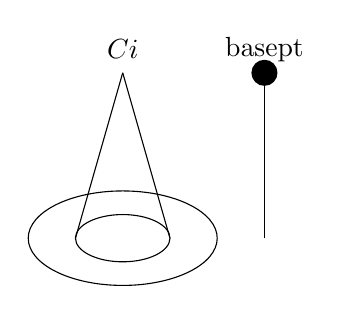
\begin{tikzpicture}[scale=0.3]
		\draw (0,0) ellipse (2 and 1);
		\draw(0,0) ellipse (4 and 2);
		\draw(2,0) -- (0,7);
		\draw(-2,0) -- (0,7);
		\node (a) at  (0,8){$Ci$};
		\node[circle,fill=black] (b) at (6,7){};
		\node (c) at (6,8){basept};

		\draw (6,0)--(6,7);
	\end{tikzpicture}
	\centering
\end{figure}
\todo{Finish picture}

\begin{note} We see that $X_+ / A_+ \cong X/A$.
\end{note}

We need to show excision and exactness (see \cite[Ch.~14]{May}). For the excision trick, it suffices to work with the theory on CW complexes, and note for a CW triad $(X,A,B)$, we have that
\begin{align*}
	A/A\cap B \to X/B
\end{align*}
is an isomorphism of CW complexes.

\end{proof}


\begin{example} We have that
\begin{align*}
	\pi_q^s (X) = \colim_k \pi_{q+k} (\Sigma^k X),
\end{align*}
which stabilizes as soon as $k>q$. Consider the functors $\pi_q^s : \Ho(\CW_\ast) \to \Ab$ for $k>q$. We get a suspension isomorphism
\begin{align*}
	\pi_q^s(X) &= \colim_k \pi_{q+k} (\Sigma^k X) \xto{\sim} \colim_k \pi_{q+k+1} (\Sigma^k X) = \pi_{q+1}^s (X),
\end{align*}
obtained by reindexing the colimit. We may use homotopy excision to show that
\begin{align*}
	(\Sigma^k X, \Sigma^k A) \to (\Sigma^k X/ \Sigma^k A \simeq \Sigma^k(X/A), \ast)
\end{align*}
is $(2k-1)$-connected. When computing $\pi_q^s$, we can look at $k$ when $k>q-1$, and look at the long exact sequence of pairs to get
\begin{align*}
	\pi_{q+k}(\Sigma^k A) \to \pi_{q+k}(\Sigma^k X) \to \pi_{q+k} (\Sigma^k (X/A))
\end{align*}
is exact at each stage in the colimit, and finally we use the fact that colimits preserve exactness.

\end{example}

\begin{remark} Colimits commute with other colimits, so in particular they commute with cokernels, which gives right exactness. As an exercise, show that left exactness holds. On the other hand, as limits commute with kernels we get left exactness,\textit{but} limits do not preserve right exactness.% TODO overflow post
\end{remark}

\begin{theorem}\label{thm:generalized-cohom} For a sequence of spaces $\{T_n\}$ with $T_n$ being $(n-1)$-connected, and with maps $\Sigma T_n \xto{\sigma_n} \Sigma T_{n+1}$, we could define
\begin{align*}
	\til{E}_q(X) := \colim_n \pi_{q+n}(X \smashprod T_n),
\end{align*}
where the colimit is taken over the composite maps
\begin{align*}
	\pi_{q+n}(X\smashprod T_n) &\xto{\Sigma} \pi_{q+n+1}(\Sigma(X\smashprod T_n)) \cong \pi_{q+n+1} (X\smashprod \Sigma T_n) \xto{\sigma_n} \pi_{q+n+1}(X\smashprod T_{n+1}).
\end{align*}
Then this defines a generalized homology theory, which satisfies all the axioms except \textit{dimension}.
\end{theorem}

\begin{remark} The example $\pi_q^s(X)$ was of the form above, where we define $T_n = \Sigma^n S^0 = S^n$, and the structure maps were the homeomorphisms
\begin{align*}
	\Sigma(\Sigma^n S^0) \cong S^{n+1} \cong \Sigma^{n+1} S^0.
\end{align*}
We note that stable homotopy does not satisfy the dimension axiom.
\end{remark}

\begin{definition} We call $\pi_q^s(S^0)$ the \textit{$q$th stable homotopy group of spheres}\index[ind]{stable homotopy groups!of spheres}. For example,
\begin{align*}
	\pi_q^s(S^0) &= \begin{cases} 0 & q<0 \\ \Z & q=0 \\ \Z\big/2 & q=1,2 \\ \Z\big/24 & q=3. \end{cases}
\end{align*}
\end{definition}

\begin{definition} A sequence of spaces $T_n$ equipped with structure maps $\sigma_n : \Sigma T_n \to T_{n+1}$ is called a \textit{(pre)spectrum}. A morphism of prespectra is a collection of maps $f_n : T_n \to T_n'$ commuting with the structure maps.\footnote{Symmetric spectra, orthogonal spectra, etc. are just prespectra equipped with additional structure.} %TODO better notation X_n, Y_n
\end{definition}

We define the \textit{homotopy groups of a prespectrum} $X$ as
\begin{align*}
	\pi_q(X) := \colim_n \pi_{q+n}(X_n).
\end{align*}

\begin{example} The \textit{suspension spectrum}\index[ind]{suspension spectrum} of a based space $X$, denoted $\Sigma^\infty X$ has $(\Sigma^\infty X)_n = \Sigma^n X$. We have that
	\begin{align*}
		\pi_q(\Sigma^\infty X) = \pi_q^s(X)
	\end{align*}
	recovers the stable homotopy of $X$. When $X = S^0$, then $\Sigma^\infty S^0 = \S$ is called the \textit{sphere spectrum}. We call $\pi_\ast (\S)$ the \textit{stable homotopy groups of spheres}.
\end{example}

\begin{customenvironment}{Digression} Consider the category $\FinSet$ of finite sets, which is equipped with a monoid structure from the operation of set union. In some sense that can be made rigorous (the Barratt-Priddy Theorem), the sphere spectrum is the group completion of $\FinSet$ with respect to set union.
\end{customenvironment}


\begin{customenvironment}{Spoiler} The \textit{Eilenberg-Maclane spaces} $\{K(\pi,n)\}$ form a prespectrum which determines singular homology with coefficients in an abelian group $\pi$.
\end{customenvironment}

\begin{note} Singular homology satisfies all axioms, including the dimension axiom (we have seen all of these axioms, except weak equivalence).
\end{note}

\begin{proposition} Let $f: X \to Y$ be $n$-connected. Then the induced map on homology
\begin{align*}
	f_\ast : H_i(X) \to H_i(Y)
\end{align*}
is an isomorphism for $i<n$ and surjective for $i=n$. In particular if $f$ is a weak equivalence, then $f$ induces an isomorphism on all homology.
\end{proposition}
\begin{proof}[Proof sketch] Note that we have CW approximations, which yield a commutative diagram
\[
	\begin{tikzcd}
	\Gamma X\dar\rar["\Gamma f" above] & \Gamma Y\dar \\
	X\rar["f" below] & Y.
	\end{tikzcd}
\]
We see that $f$ is $n$-connected if and only if $\Gamma f$ is $n$-connected. Therefore without loss of generality, we may assume that $X$ and $Y$ are CW complexes. Recall by the strong version of Whitehead's theorem, %todo cite
we have that
\begin{align*}
	f_\ast : [W,X] \to [W,Y]
\end{align*}
is a bijection if $\dim(W)<n$ and a surjection if $\dim(W) = n$. Take $W = Y^{(n)}$ to be the $n$-skeleton of $Y$. Then we have that
\begin{align*}
	f_\ast : [Y^{(n)} , X] \to [Y^{(n)}, Y]
\end{align*}
is onto, so there exists $g: Y^{(n)} \to X$ such that the following diagram commutes up to homotopy:
\[
	\begin{tikzcd}
	X\rar["f" above] & Y \\
	 & Y^{(n)}\ar[ul,"g" below left]\uar["i_n" right].
	\end{tikzcd}
\]
Thus since $i_n$ is surjective on $H_k$ for $k\leq n$, so is $f$. As an exercise, show that $f$ is injective on homology.

\end{proof}

\begin{customenvironment}{Upshot} We may prove things about singular homology of all spaces by only using singular homology of CW complexes.
\end{customenvironment}

There is a link between homology and homotopy groups:

\begin{definition} The \textit{Hurewicz homomorphism}\index[ind]{Hurewicz homomorphism} is a group homomorphism
\begin{align*}
	h : \pi_n(X) \to \til{H}_n(X),
\end{align*}
where a map $S^n \to X$ corresponds to a map $\Delta^n \to X$ where $\del\Delta^n \to \ast$. This corresponds to a cycle in $C_n^{sing}(X)$, which yields an element in $\til{H}_n(X)$.
% TODO perfect pairing definition
\end{definition}

\begin{theorem} The Hurewicz homomorphism is a natural homomorphism which is compatible with suspension \cite[15.1]{May}, \cite[2.A]{Hatcher}.
\end{theorem}

\begin{theorem} Any reduced homology theory on CW complexes (equivalently, spaces) satisfying axioms (1)---(4) and (5) the dimension axiom is isomorphic as a homology theory to singular homology.
\end{theorem}
\begin{proof}[Proof idea] Suppose  that $X$ is a CW complex, and $H_\ast$ is some given homology theory satisfying all the axioms, including the dimension axiom. Let $C_n(X) = H_n(X^{(n)}, X^{(n-1)}) \cong \til{H}_n(X^{(n)}/X^{(n-1)})$, together with $d : C_n (X) \to C_{n-1}(X)$ defined by the composite
\begin{align*}
	H_n(X^{(n)}, X^{(n-1)}) \xto{\del} H_{n-1}(X^{(n-1)}) \to H_{n-1}( X^{(n-1)}, X^{(n-2)}).
\end{align*}
We may check that $d\circ d = 0$.
\end{proof}

\begin{theorem} We have that $C_\ast (X) \cong C_\ast^{cell}(X)$ as chain complexes.
\end{theorem}
We see $C_n(X) \cong C_n^{cell}(X)$ by additivity since $X^{(n)}/X^{(n-1)} \simeq \wedge S^n$, where the wedge is taken over the $n$-cells of $X$. To reconcile the differentials between these chain complexes, we need the Hurewicz homomorphism \cite[15.2]{May}.

\begin{theorem} We have then that $H_\ast(X,A) \cong H_\ast (C_\ast (X,A))$ (where $C_\ast(X,A):= C_\ast(X)/C_\ast(A)$) such that differentials agree \cite[15.2]{May}.
\end{theorem}
It suffices to show this previous theorem on CW complexes.

Finally, by dimension, suspension, and additivity, if we know the value of our homology theory on spheres, then the entire homology theory is determined by its value on $S^0$. The dimension axiom yields the equivalence with singular homology.
\hfill\qed

% Lecture 15: March 19th

% There is no finite-dimensional simply connected complex all of whose homotopy groups we know.


\subsection{Generalized cohomology theories}
\begin{definition} A \textit{reduced generalized cohomology theory}\index[ind]{cohomology theory!reduced} $\til{E}^\ast$ consists of contravariant functors
\begin{align*}
	\til{E}^q : \Ho(\Top_\ast) \to \Ab
\end{align*}
from the homotopy category of well-based spaces to abelian groups satisfying
\begin{enumerate}
	\item \textit{exactness}: if $A\cofto X$ is a cofibration, then
	\begin{align*}
		\til{E}^q(X/A) \to \til{E}^q(X) \to \til{E}^q(A)
	\end{align*}
	is exact

	\item \textit{suspension}: there exist natural isomorphisms
	\begin{align*}
		\til{E}^q(X) \cong \til{E}^{q+1}(\Sigma X)
	\end{align*}

	\item \textit{additivity}: if $X = \bigwedge_i X_i$, then the maps $X_i \to X$ induce an isomorphism
	\begin{align*}
		\til{E}^q(X) \xto{\sim} \prod_i \til{E}^q(X_i)
	\end{align*}

	\item \textit{weak equivalence}: if $f:X\to Y$ is a weak equivalence, then $f^\ast : \til{E}^q(Y) \to \til{E}^q(X)$ is an isomorphism.
\end{enumerate}
Additionally, for a fixed abelian group $\pi$, we have a further axiom that may or may not be satisfied
\begin{enumerate}\setcounter{enumi}{4}
	\item \textit{dimension}: we have that
	\begin{align*}
		\til{E}^q(S^0) = \begin{cases} \pi & q=0 \\ 0 & q\neq 0. \\ \end{cases}
	\end{align*}
\end{enumerate}
\end{definition}

Similarly as for homology:
\begin{itemize}
	\item it determines and is determined by a theory on based CW complexes
	\item it determines and is determined by an unreduced theory on pairs satisfying long exact sequences, excision, additivity, weak equivalences, and maybe dimension. Moreover for the unreduced theory, a similar theory on CW pairs exists.
\end{itemize}

\begin{theorem} Singular cohomology is the unique cohomology theory satisfying (1)---(4) and the dimension axiom.
\end{theorem}

\begin{remark} A reduced cohomology theory $\til{E}$ includes the data of a natural transformation of functors $\til{E}^n \circ \Sigma \Rightarrow \til{E}^{n+1}$.
\end{remark}


\begin{customenvironment}{Question}\label{q:cohom-thy} Can we find other cohomology theories? How do we recover singular cohomology? Is there a sequence of spaces $\{P_n\}$ such that $[-,P_n]_\ast$ is a generalized cohomology theory?
\end{customenvironment}


Let $Z$ be a based space of the homotopy type of a CW complex, and consider the functor
\begin{align*}
	[-,Z]_\ast : \CW_\ast^\op \to \Set_\ast.
\end{align*}
This has the following properties
\begin{itemize}
	\item it clearly satisfies \textit{homotopy invariance}, since if $f,g: X\to Y$ are homotopic maps, then $f^\ast = g^\ast$ as maps
	\begin{align*}
		[Y,Z]_\ast \to [X,Z]_\ast.
	\end{align*}

	\item we have \textit{exactness} for the inclusion of a subcomplex $A\subseteq X$. That is,
	\begin{align*}
		[X/A,Z]_\ast \to [X,Z]_\ast \to [A,Z]_\ast
	\end{align*}
	is exact, as we have seen before % todo find link

	\item \textit{additivity}: for $X = \bigwedge_i X_i$, we have an isomorphism
	\begin{align*}
		[X,Z]\ast = \left[ \bigwedge_i X_i, Z\right]_\ast \xto{\simeq} \prod_i [X_i, Z]_\ast
	\end{align*}
	by the universal properties of products and coproducts.
\end{itemize}

This satisfies all the axioms of a cohomology theory except the suspension axiom. In order to build a cohomology theory from $[-,Z]_\ast$, we will need to check when this last axiom holds. We will also need to verify that $[X,Z]_\ast$ is a group, rather than just a set. Recall that we have a natural isomorphism
\begin{align*}
	[\Sigma X, Y]_\ast \cong [X, \Omega Y]_\ast.
\end{align*}

\begin{definition} An \textit{$H$-space (Hopf space)}\index[ind]{$H$-space} is a topological space $X$ equipped with a ``multiplication map''
\begin{align*}
	\mu: X\times X \to X,
\end{align*}
and a two sided identity $e\in X$. Alternatively, we might ask for $\mu(-,e)$ and $\mu(e,-)$ to be homotopic to the identity $\id_X$. This operation is called \textit{homotopy associative} if the diagram commutes up to homotopy:
\[
	\begin{tikzcd}
	X\times X\times X \rar["\mu\times \id" above]\dar["\id\times\mu" left] & X\times X\dar["\mu" right] \\
	X\times X \rar["\mu" below] & X.
	\end{tikzcd}
\]
The operation is called \textit{homotopy commutative} if the diagram commutes up to homotopy
\[
	\begin{tikzcd}
	X\times X\rar["\mu"]\dar["\text{swap}" left] & X \\
	X\times X.\ar[ur,"\mu" below right] &
	\end{tikzcd}
\]
\end{definition}

\begin{proposition} The set $[X,Z]_\ast$ has the structure of an abelian monoid if $Z$ is a homotopy associative and commutative $H$-space. This set is furthermore an abelian group if $Z$ is \textit{grouplike}\index[ind]{grouplike space}, that is if the multiplication $\mu$ on $Z$ induces a group structure on $\pi_0(Z)$. We may impose the stronger condition that we have inverses up to homotopy; that is, we have an ``inversion'' map $\chi : Z\to Z$ such that the diagram commutes up to homotopy:
\[
	\begin{tikzcd}
	Z\times Z\rar["\id\times\chi"] & Z\times Z\ar[d,"\mu" right]\\
	Z\ar[u,"\Delta" left]\rar["\const_{e}" below] & Z.
	\end{tikzcd}
\]
\end{proposition}

\begin{exercise} For any space $Y$, we have that $\Omega Y$ is a grouplike homotopy associative $H$-space, and $\Omega^2 Y$ is a grouplike homotopy associative and commutative $H$-space.
\end{exercise}

Returning to Question \ref{q:cohom-thy}, we see that it suffices to pick $P_n$ to be $\Omega^2$ of some other space for each $n$, and we also need that $\til{E}^n(X) = \til{E}^{n+1}(\Sigma X)$, that is,
\begin{align*}
	[X,P_n]_\ast &\cong [\Sigma X, P_{n+1}]_\ast \cong [X,\Omega P_{n+1}]_\ast.
\end{align*}
From this we see it suffices to define $\{P_n\}$ by letting the adjoint maps to the structure maps $P_n \xto{\sim} \Omega P_{n+1}$ be weak equivalences.

\begin{definition} A (pre)spectrum $\{P_n\}$ is called an \textit{$\Omega$-(pre)spectrum}\index[ind]{$\Omega$-spectrum} if the adjoints of the structure maps are weak equivalences.
\end{definition}

\begin{remark} We have shown that for every $\Omega$-prespectrum $P_\bullet$, the functor
\begin{align*}
	h_n : \CW_\ast &\to \Ab \\
	X &\mapsto [X,P_n]_\ast
\end{align*}
defines a generalized cohomology theory.
\end{remark}

\begin{customenvironment}{Question} Is every generalized cohomology theory of this form?
\end{customenvironment}

Yes! By Brown representability.

\begin{customenvironment}{Warning} The homotopy category of spectra and the category of generalized cohomology theories are not equivalent. We can have a non-nullhomotopic map of spectra which induces the zero map on corresponding cohomology theories, see \cite{mo-hyperphantoms}.
\end{customenvironment}

% TODO hyperphantoms \href{https://mathoverflow.net/questions/117684/are-spectra-really-the-same-as-cohomology-theories}{Overflow post}

\begin{note} Not all (pre)spectra are $\Omega$-spectra. For example, suspension (pre)spectra are not $\Omega$-spectra (in particular $\S$ is not an $\Omega$-spectrum).

But for any (pre)spectrum $P_\bullet$, we may replace $P_n$ by $\colim_k \Omega^k P_{n+k}$, which is an $\Omega$-(pre)spectrum. We define the cohomology theory
\begin{align*}
	h^n(X):= \left[X, \colim_k \Omega^k P_{n+k}\right]_\ast.
\end{align*}
\end{note}

\begin{example} Bott periodicity, in complex $K$-theory, is the result that $\BU \simeq \Omega^2 \BU$. Thus we define an $\Omega$-(pre)spectrum $\BU_\bullet = \{\BU, \Omega \BU, \BU, \Omega \BU,\ldots\}$, which yields a cohomology theory, called complex topological $K$-theory.
\end{example}

% Lecture 16: March 26th
\textbf{Plan}: For an abelian group $\pi$, we want to define spaces $K(\pi,n)$ such that
\[
    \pi_q(K(\pi,n)) = \begin{cases} \pi & q=n \\ 0 & \text{otherwise}. \end{cases}
\]

Let's start with $K(\pi,1)$, which works for all $\pi$ (not necessarily abelian). This is also called the \textit{bar construction}.

\begin{customenvironment}{Idea for the bar construction} We define $BG$ to be the configuration space of $n+1$ points in the unit interval $I$, over all natural numbers $n$ such that
\begin{align*}
    0\leq g_0 \leq g_1 \leq \cdots \leq g_n \leq 1.
\end{align*}
We subject this configuration space to the following relations:
\begin{itemize}
    \item if $g_0 = 0$, then we define an equivalence
\begin{align*}
    (0=g_0, g_1,\ldots,g_n) \sim (g_1,\ldots, g_n).
\end{align*}

    \item if $g_n = 1$, we similarly have
\begin{align*}
    (g_0,\ldots,g_n=1) \sim (g_0,\ldots,g_{n-1}).
\end{align*}

    \item if $g_i = e$ is the identity element of $G$, then we say that
        \begin{align*}
            (g_0,\ldots,g_{i-1},e,g_i,\ldots,g_n) \sim (g_0,\ldots,g_{i-1},g_{i+1},\ldots,g_n).
        \end{align*}

    \item finally, we require that
    \begin{align*}
    (g_0,\ldots,g_{i-1},g_i,\ldots,g_n) \sim (g_0,\ldots,g_{i-2}, g_{i-1}\cdot g_i, g_{i+1},\ldots, g_n).
    \end{align*}
\end{itemize}

\end{customenvironment}

\ifx
We want configurations of points in $I$, labeled by elements in $G$, such that
    \begin{itemize}
        \item when points collide, labels combine using multiplication in $G$
        \item points can slide off to infinity.
    \end{itemize}
\end{customenvironment}

That is, subdivisions of the unit interval, where $t_i$ denotes some small length, $g_i \in G$ is a group element, and we have that $\sum_i t_i = 1$:
\begin{center}
\begin{tabular}{|c|c|c|c|c|}
    $t_0$ & $t_1$ & $t_2$ & $\cdots$ & $t_n$ \\
    \hline
    $g_0$ & $g_1$ & $g_2$ & $\cdots$ & $g_n$ \\
\end{tabular}
\end{center}
This is subject to the following identifications:
\begin{center}
\begin{tabular}{|c|c|c|c|c|c|c|c|c|}
    $t_0$ & $t_1$ & $\cdots$ & $t_{i-1}$ & $0$ & $t_i$ & $\cdots$ & $t_{n-1}$ \\
    \hline
    $g_0$ & $g_1$ & $\cdots$ & $g_{i-1}$ & $g_i$ & $g_{i+1}$ & $\cdots$ & $g_n$
\end{tabular} $\ \sim\ $
\begin{tabular}{|c|c|c|c|c|c|c|c|c|}
    $t_0$ & $t_1$ & $\cdots$ & $t_{i-1}$ & $t_i$ & $\cdots$ & $t_{n-1}$ \\
    \hline
    $g_0$ & $g_1$ & $\cdots$ & $g_{i-1}$ & $g_i g_{i+1}$ & $\cdots$ & $g_n$
\end{tabular},
\end{center}
and
\begin{center}
\begin{tabular}{|c|c|c|c|c|c|c|c|c|}
    $0$ & $t_0$ & $t_1$ & $\cdots$ & $t_{n-1}$ \\
    \hline
    $g_0$ & $g_1$ & $g_2$ & $\cdots$ & $g_n$
\end{tabular} $\ \sim\ $
\begin{tabular}{|c|c|c|c|c|c|c|c|c|}
    $t_0$ & $t_1$ & $t_2$ & $\cdots$ & $t_{n-1}$ \\
    \hline
    $g_1$ & $g_2$ & $g_3$ & $\cdots$ & $g_n$
\end{tabular},
\end{center}
and similarly if 0 is at the end, and finally that we are allowed to concatenate lengths by multiplication by the identity in the group:
\begin{center}
\begin{tabular}{|c|c|c|c|c|c|c|c|c|}
    $t_0$ & $t_1$ & $\cdots$ & $t_{i-1}$ & $t_i$ & $t_{i+1}$ & $\cdots$ & $t_{n}$ \\
    \hline
    $g_0$ & $g_1$ & $\cdots$ & $g_{i-1}$ & $e$ & $g_{i+1}$ & $\cdots$ & $g_n$
\end{tabular} $\ \sim\ $
\begin{tabular}{|c|c|c|c|c|c|c|c|c|}
    $t_0$ & $t_1$ & $\cdots$ & $t_{i-1}$ & $t_i + t_{i+1}$ & $\cdots$ & $t_{n}$ \\
    \hline
    $g_0$ & $g_1$ & $\cdots$ & $g_{i-1}$ & $g_{i+1}$ & $\cdots$ & $g_n$
\end{tabular}
\end{center}



Observe that $BG = \coprod_{n=0}^\infty G^n \times \Delta^n / \sim$. %TODO clean this up
\fi


Let $\DDelta$ denote the category whose objects are finite nonempty totally ordered sets $[n] = \{0<1< \cdots < n\}$, and morphisms are order preserving functions.

\begin{definition} A \textit{simplicial set}\index[ind]{simplicial set} is a contravariant functor $\DDelta \to \Set$, that is, a functor $\DDelta^\op \to \Set$. A morphism of simplicial sets is a natural transformation of these functors.This gives us a category, denoted $\sSet$.
\end{definition}

\begin{remark} We may define a simplicial object in any category $\mathscr{C}$ as a functor
    \[
        \DDelta^\op \to \mathscr{C}.
    \]
\end{remark}

\begin{note} The category $\DDelta$ has a generating set of morphisms. For all $n\ge 0$,
\begin{itemize}
    \item there exist $n+1$ injections $d^i : [n-1] \to [n]$ for $0\leq i\leq n$, which ``skips'' $i$, that is,
        \[
            d^i(k) = \begin{cases} k & k<i \\ k+1 & k\geq i, \end{cases}
        \]
        called the \textit{coface maps}. %TODO check
\end{itemize}
There exist $n+1$ surjections $s^j : [n+1] \to [n]$ for $0\leq j\leq n$, which ``repeat'' $j$, that is,

\[
    s^j(k) = \begin{cases} k & k\leq j \\ k-1 & k>j \end{cases}
\]
\end{note}

\begin{remark} These satisfy
    \begin{align*}
        d^j d^i &= d^i d^{j-1} \quad\text{for } i<j \\
        s^j s^i &= s^i s^{j+1} \quad\text{for }  i\leq j \\
        s^j d^i &= \begin{cases} \id & \text{for } i=j,\ i=j+1 \\ d^i s^{j+1} &\text{for } i<j \\ d^{i-1} s^j &\text{for } i>j+1. \end{cases}
    \end{align*}
\end{remark}
Moreover, every morphism in $\DDelta$ can be written as a composite of $s^i$'s and $d^j$'s.

For $X\in \sSet$, we obtain a set $X_n$ for all $n\geq 0$, and we have maps $d_i := X(d^i) : X_n \to X_{n-1}$ for $0\leq i\leq n$, called \textit{face maps}, and we have maps $s_j = X(s^j):X_n \to X_{n+1}$ for $0\leq j\leq n$, called \textit{degeneracy maps}, which satisfy relations dual to those above.

\begin{definition} A simplicial set $X_\dot$ may be defined alternatively as a collection of sets $X_0,X_1,\ldots$ together with functions $d_i: X_n \to X_{n-1}$ and $s^j: X_n \to X_{n+1}$ satisfying the relations:
\begin{align*}
    d_i d_j &= d_{j-1} d_i \quad \text{for } i<j \\
    s_i s_j &= s_{j+1} s_i \quad \text{for } i\leq j \\
    d_i s_j &= \begin{cases} \id & \text{for } i=j,\ i=j+1 \\ s_{j-1}d_i & \text{for } i<j \\ s_j d_{i-1} & \text{for } i>j+1. \end{cases}
\end{align*}
\end{definition}

A map of simplicial sets $f_\dot : X_\dot \to Y_\dot$ is a collection of functions $f_n : X_n \to Y_n$ that commute with the face and degeneracy maps.

\begin{customenvironment}{References} For a nice introduction to simplicial sets, see \cite{friedman4221elementary} or \cite{riehl-sset}. A more in-depth treatment of simplicial homotopy theory is given in \cite{goerss-jardine}.
\end{customenvironment}

\begin{example} The singular complex of a space $X$. We first define the topological $n$-simplex as
    \[
        \Delta^n := \{(t_0, \ldots, t_n) \in \R^{n+1} \ : 0\leq t_i\leq 1,\ \sum_{i=0}^n t_i = 1\}.
    \]

    Note that we have canonical maps for $0\leq i\leq n$
    \begin{align*}
        \sigma_j : \Delta^{n} &\to \Delta^{n+1} \\
        (t_0,\ldots,t_n) &\mapsto (t_0,\ldots,t_{i-1},0,t_i,\ldots,t_n).
    \end{align*}
    Which we may think about as viewing an $(n-1)$-simplex as a degenerate $n$-simplex, and we have another map for $0\leq i\leq n$
    \begin{align*}
        \delta_i : \Delta^{n} &\to \Delta^{n-1} \\
        (t_0,\ldots,t_{n}) &\mapsto (t_0,\ldots,t_{i-1}, t_i + t_{i+1},\ldots,t_{n}),
    \end{align*}
    which we think of as projecting onto the $(n-1)$-simplex orthogonal to the $i$th face.
\end{example}

\begin{definition} Let $X$ be a topological space. Then $\Sing(X)$ is the simplicial set with $n$-simplices $\Sing(X)_n = \Top(\Delta^n, X)$ to be the set of continuous maps $\Delta^n \xto{f} X$. This comes with face and degeneracy maps given by
\begin{align*}
    d_i : \Top(\Delta^{n}, X) &\to \Top(\Delta^{n-1}, X) \\
    (\Delta^{n} \xto{f} X) &\mapsto (\Delta^{n-1} \xto{\sigma_i} \Delta^{n} \xto{f} X),
\end{align*}
and
\begin{align*}
    s_j : \Top(\Delta^{n}, X) &\to \Top(\Delta^{n+1}, X) \\
    (\Delta^{n} \xto{f} X) &\mapsto (\Delta^{n+1} \xto{\delta_j} \Delta^{n} \xto{f} X).
\end{align*}
\end{definition}

\begin{remark} This functor is used to define singular homology:
\begin{align*}
    H_n(-,\Z) : \Top \xto{\Sing(-)} \sSet \xto{F} \sAb \to \Ch_\Z,
\end{align*}
where $F$ takes a free abelian group on each $X_n$, and we have that $\delta:= \sum (-1)^i d_i$ in $\Ch_\Z$.
\end{remark}

\begin{definition} Let $\mathscr{C}$ be a small category. The \textit{nerve of $\mathscr{C}$}\index[ind]{nerve of a category}, denoted $N\mathscr{C}$ is the simplicial set with
\begin{align*}
    (N\mathscr{C})_0 &= \ob\mathscr{C} \\
    (N\mathscr{C})_1 &= \mor \mathscr{C} \\
                     &\vdots \\
    (N\mathscr{C})_n &= \{\text{strings of $n$-composable morphisms}\}.
\end{align*}
We have degeneracy maps $s_j : (N\mathscr{C})_n \to (N\mathscr{C})_{n+1}$ inserting an identity at the $j$th slot,and we get face maps $d_i : (N\mathscr{C})_n \to (N\mathscr{C})_{n-1}$ which, for $0\leq i\leq n-1$, composes the $i$ and $i+1$st morphism, and $d_n$ omits the last maps, respectively.
\end{definition}

\begin{customenvironment}{Observation} If we have a group $G$, it is a category with one object, and composition is given by the group multiplication. Its nerve has $(NG)_n = G^n$, whose face maps $d_i : G \to G^{n-1}$ are given by multiplication at slot $i$, for $0<i<n$, and for $d_0$ and $d_n$ forget the $0$th and $n$th entry, respectively. The degeneracy maps $s_i$ insert the identity $e$ at slot $i$.\todo{We should be consistent in $d_i$, $s_j$, etc. I think this is a common thing in the literature to use different indexing notation.}

\end{customenvironment}

% Lecture 17: March 28th


\begin{example} If $X$ is a right $G$-space, and $Y$ is a left $G$-space, we define the simplicial set $B_\dot (X,G,Y)$ with
\[
    B_n(X,G,Y) := X \times G^n \times Y,
\]
and face and degeneracy maps
\begin{align*}
    d_i(x,g_0,\ldots,g_{n-1},y) &= \begin{cases} (x,g_1,\ldots,g_i\cdot g_{i+1},\ldots, g_{n-1},y) & 0<i<n \\
    (x\cdot g_0, g_1,\ldots,g_{n-1},y) & i=0 \\
    (x,g_0,\ldots,g_{n-2}, g_{n-1}\cdot y) & i=n,\end{cases} \\
    s_i(x,g_0,\ldots,g_{n-1},y) &= (x,g_0,\ldots,g_{i-1},e,g_i,\ldots,g_{n-1},y).
\end{align*}
The previous example $BG$ is just $B(\ast, G, \ast)$.
\end{example}

\subsection{Geometric realization}
\begin{definition} Let $X_\dot$ be a simplicial set. Then its \textit{geometric realization}\index[ind]{geometric realization} is given by
\begin{align*}
    |X_\dot| := \coprod_{n\ge 0} X_n \times \Delta^n \Big/\sim,
\end{align*}
where the equivalence relation is given by
\begin{align*}
    (x, \delta_i u) &\sim (d_i x, u) \quad \quad x\in X_n,\ u\in \Delta^{n-1},\\
    (y,\sigma_i v) &\sim (s_i y, v) \quad \quad y\in X_{n-1},\ v\in \Delta^n,
\end{align*}
and whose topology is the quotient topology.
\end{definition}

\begin{customenvironment}{Intuition} Out of this simplicial set $X_\dot$, we woudl like to build a topological space which records the combinatorial data of the simplicial set in a topological way. More specifically, we will build a CW complex whose 0-cells are precisely $X_0$, and whose higher cells are non-degenerate simplices, that is, our $n$-cells should not arise as the degeneracy of some lower-dimensional information.
\end{customenvironment}

\begin{definition} An $n$-simplex is called \textit{nondegenerate}\index[ind]{simplex!nondegenerate} if it cannot be written as $s_i y$ for any $y\in X_{n-1}$ for any $i$.
\end{definition}

\begin{note} We have that $|-|: \sSet \to \Top$ is a functor.
\end{note}

\begin{example} The space $|\Sing(X)|$ is huge, and comes equipped with a map
    \begin{align*}
        \gamma : |\Sing(X)| &\to X \\
       \left[ \Delta^n \xto{f} X,\ u\in \Delta^n \right] &\mapsto f(u).
    \end{align*}
\end{example}

 \todo{cite Milnor's original paper}

\begin{theorem}[{\cite{Milnor}, \cite[16.2]{May}}] This morphism $\gamma$ is a weak equivalence. Moreover, $|\Sing(X)|$ is a CW complex with one $n$-cell for each nondegenerate $n$-simplex of $X$.
\end{theorem}

\begin{note} The map $\gamma$ is a natural transformation $|\Sing(-)| \Rightarrow \id_{\Top}$.
\end{note}


\begin{proposition} If $z$ is a degenerate simplex, that is, $z = s_i x$ for some $x_i$ and some (possibly nondegenerate) $x$, then there is a unique nondegenerate simplex $y$ such that
\begin{align*}
    z = s_{i_1} \cdots s_{i_k} = y,
\end{align*}
for some $s_{i_1} \ldots s_{i_k}$.
\end{proposition}

\begin{theorem} The functors $|-|$ and $\Sing(-)$ are adjoints. That is, for $X\in \sSet$ and $Y\in \Top$, there is a natural isomorphism
\begin{align*}
    \Hom_\Top (|X|,Y) \cong \Hom_\sSet (X, \Sing(Y)).
\end{align*}
\end{theorem}

\begin{proof}[Proof idea] We define a map
\begin{align*}
    \phi : \Hom_\sSet (X, \Sing(Y)) \to \Hom_\Top (|X|, Y),
\end{align*}
by taking a morphism of simplicial sets $X\xto{f} \Sing(Y)$ .... \todo{finish this proof}

\end{proof}


\begin{examples} $\ $
\begin{enumerate}
    \item the \textit{classifying space}\index[ind]{classifying space} of a small category $\mathscr{C}$, denoted $B\mathscr{C}$, is defined by
    \begin{align*}
        B\mathscr{C} := |N \mathscr{C}|.
    \end{align*}

    \item we have that $B(X,G,Y):= |B_\dot (X,G,Y)|$.

    \item the space $BG$ is a particular example of both of the above examples;
        \begin{itemize}
            \item $G$ is a category with one object
            \item $G = B(\ast, G,\ast)$.
        \end{itemize}
\end{enumerate}
\end{examples}

\begin{customenvironment}{Easy example} The classifying space of the single object category, that is, the trivial group $\{e\}$, is the topological space with a single point.
\end{customenvironment}


\begin{exercise} We have that $B(\Z\big/2) \cong \RP^\infty$.
\end{exercise}

\begin{exercise} If we have a category $\dot \to \dot$, its classifying space is the unit interval $I=[0,1]$.
\end{exercise}

\begin{definition} We define the space $EG$ to be the geometric realization of the simplicial set $E_\dot G$, defined by
\begin{align*}
    E_n G := G^{n+1},
\end{align*}
with face and maps defined by
\begin{align*}
    d_i(g_1,\ldots,g_{n+1}) &= \begin{cases} (g_2,\ldots,g_{n+1}) & i=0 \\ (g_1,\ldots,g_{i-1}, g_i\cdot g_{i+1},\ldots,g_{n+1}) & 1\leq i\leq n, \end{cases} \\
    s_j(g_1,\ldots,g_{n+1}) &= (g_1,\ldots,g_{i-1},e, g_i,\ldots,g_{n+1}), \quad 0\leq i\leq n.
\end{align*}
\end{definition}

We note that this simplicial set is just $B(\ast, G, G)$. We obtain a map of simplicial sets
\begin{align*}
    p_n : E_n G \to B_n G,
\end{align*}
given by projection on the first $n$ coordinates. This commutes with face and degeneracy maps (check). Therefore by functoriality, we get a continuous map
\begin{align*}
    p : EG \to BG.
\end{align*}

Let $G$ act on $E_n G$ on the right:
\[
    (g_1,\ldots,g_{n+1})\cdot g:= (g_1,\ldots,g_n, g_{n+1}\cdot g),
\]
then $E_\dot G$ is a simplicial $G$-set, and the $G$-action commutes with the face and degeneracy maps, so $EG$ is a $G$-space. We note also that modding by this action, we obtain $E_n G/G = B_n G$. We claim that this quotient passes to the geometric relation (since colimits commute), thus $BG = EG/G$.

\begin{theorem}[{\cite[16]{May}}] We have that $p: EG \to BG$ is a bundle with fiber $G$. Moreover, every principal $G$-bundle is a pullback of the form
\[
    \begin{tikzcd}
        E\rar\dar\pb & EG\dar["p" right] \\
    X\rar & BG.
    \end{tikzcd}
\]
That is, $EG\to BG$ is the \textit{universal principal $G$-bundle}.
\end{theorem}

\begin{exercise} We have that $EG\simeq \ast$ is contractible. Thus by the long exact sequence, we see that
\begin{align*}
    \pi_{q+1}(BG) \cong \pi_q(G).
\end{align*}
This holds for any topological group. In particular, for $G$ discrete, we have that
\begin{align*}
    \pi_1(BG) &\cong \pi_0(G) = G,\\
    \pi_n(BG) &\cong 0,
\end{align*}
for any $n \neq 1$. Thus $BG = K(G,1)$.
\end{exercise}

\begin{theorem}[Milnor] We have that $|-|: \sSet \to \Top$ preserves products, that is,
\begin{align*}
    |X_\dot \times Y_\dot| \cong |X_\dot| \times |Y_\dot|.
\end{align*}
\end{theorem}

As a corollary, we see that $B(G\times H) \cong BG \times BH$. That is, the functor $B:\Top\Grp \to \Top$ preserves products. When $G$ is abelian, the multiplication map $\mu: G\times G \to G$ is abelian, thus $BG$ becomes a topological group.\footnote{Since $B: \Top\Grp \to \Top$ preserves products and the terminal object, it sends group objects to group objects, that is, topological abelian groups to topological groups.}

Thus for $G$ abelian, we may iterate this construction to define $B^n G := B(B^{n-1} G)$. Moreover for $G$ discrete and abelian, we see that
\begin{align*}
    \pi_q(B^n G) = \pi_{q-n}(G) =  \begin{cases} G & q=n \\ 0 & \text{otherwise}. \end{cases}
\end{align*}

Therefore $K(G,n) = B^n G$.














\newpage
\listoftodos
\newpage
\end{comment}









%%%%%%%

\appendix
% Appendix

% Thomas, 2/2 -- feel free to delete this
\section{More category theory: properties of morphisms}

As we have seen, limits and colimits allow us ways to construct new objects, morphisms, and universal properties, over indexing diagrams. In particular we might be interested in relating certain properties of morphisms in a category to induced morphisms produced out of a colimit. As a motivating example, consider the following question.

\begin{question} Let $I$ be a small indexing diagram, and let $\alpha,\beta: I \to \Set$ denote two functors, and let $A_i := \alpha(i)$ and $B_i = \beta(i)$ denote the sets at each object $i\in I$. Suppose we have a natural transformation between these functors, consisting of functions $f_i \colon A_i \to B_i$ for each $i$. \textit{If each $f_i$ is injective, is it true that the induced map $f\colon \colim \alpha \to \colim \beta$ is injective as well?}
\end{question}

It turns out the answer to this diagram depends on the shape of $I$. It is true if the colimits are \textit{filtered}, which is a condition on the indexing diagram which tells us that it interacts well with finite limits. This motivates the more broad question of what properties of morphisms are preserved under limits and colimits. In general this is a hard question, but it will be important when we investigate fibrations and cofibrations in the category of topological spaces.


\subsection{Stability and closure definitions}



Let $\mathscr{C}$ be a category, not necessarily assumed to be locally small. We start with an easy definition.

\begin{definition}\label{def:closed-under-pullback} Let \textbf{P} be a property of morphisms in $\mathscr{C}$. We say that \textbf{P} is \textit{closed under composition} if, anytime we have two composable morphisms $f: x \to y$ and $g: y \to z$, if both $f$ and $g$ have property \textbf{P}, then the composite $g\circ f$ does as well.
\end{definition}


\begin{definition}\label{def:2-out-of-3} Let \textbf{P} be a property of morphisms in $\mathscr{C}$. We say that \textbf{P} \textit{satisfies 2-out-of-3} if for every commutative diagram of the form
\[ \begin{tikzcd}
    A\rar["f" above]\ar[dr,"g\circ f" below left] & B\dar["g" right]\\
     & C,\\
\end{tikzcd} \]
if any two of $f$, $g$, or $g\circ f$ have property \textbf{P}, then the third does as well.
\end{definition}


\begin{exercise} $\ $
\begin{enumerate}
    \item Prove that isomorphisms satisfy 2-out-of-3.
    \item In the category $\Set$, prove that injections and surjections do not satisfy 2-out-of-3.
\end{enumerate}
\end{exercise}

\begin{definition}\label{def:cancellative-properties} Let \textbf{P} be a property of morphisms.
\begin{enumerate}
    \item We say that \textbf{P} is a \textit{left cancellative property} if any time $g\circ f$ has property \textbf{P}, this implies that $f$ has property \textbf{P} as well.
    \item We say that \textbf{P} is a \textit{right cancellative property} if any time $g\circ f$ has property \textbf{P}, this implies that $g$ has property \textbf{P} as well.
\end{enumerate}
\end{definition}
As a warning to the reader, \textbf{the terminology in} \autoref{def:cancellative-properties} \textbf{is not standard}, although we would advocate for its usage. The notion of left cancellative properties is referred to as (CANC) in \cite[Appendix~C]{GortzWedhorn}, and has many examples in algebraic geometry (e.g. immersions, locally of finite type, purely inseparable, quasi-separated, separated). Many other examples occur under hypotheses on $g$, e.g. if it is separated or unramified. In a broader categorical context, we will see that mono-(resp. epi-)morphisms are left (resp. right) cancellative. 


\begin{definition}\label{def:closed-under-retracts} Let \textbf{P} be a property of morphisms. We say that \textbf{P} is \textit{closed under retracts} if, for any $f: A \to B$ with property \textbf{P}, and any $g: X \to Y$ fitting into a commutative diagram
\[ \begin{tikzcd}
    X\ar[rr,bend left=30,"\id_X" above]\dar["g" left]\rar & A\dar["f"]\rar & X\dar["g" right]\\
    Y\rar\ar[rr,bend right=30,"\id_Y" below] & B\rar & Y,
\end{tikzcd} \]
we have that $g$ has property \textbf{P} as well.
\end{definition}







\begin{definition} Let \textbf{P} be a property of morphisms. Then we say that \textbf{P} is \textit{stable under pullback} (often also called \textit{stable under base change}) if for any pullback diagram of the form
\[ \begin{tikzcd}
    C\rar["j" above]\dar["k" left]\pb & D\dar["f" right]\\
    A\rar["g" below] & B,\\
\end{tikzcd} \]
if $f$ has property \textbf{P}, then $k$ has property \textbf{P} as well. Dually, we say that \textbf{P} is \textit{stable under pushout} if for any pushout diagram of the form
\[ \begin{tikzcd}
    C\rar["j" above]\dar["k" left] & D\dar["f" right]\\
    A\rar["g" below] & B\po,\\
\end{tikzcd} \]
if $k$ has property \textbf{P}, then $f$ has property \textbf{P} as well.
\end{definition}

\begin{exercise}\label{exer:injective-stable-under-pullback} $\ $
\begin{enumerate}
    \item Prove that isomorphisms are always stable under pushout and pullback.
    \item Prove in the category $\Set$ that injective functions are stable under pullback, and surjective functions are stable under pushout.
\end{enumerate}
\end{exercise}


Thus far we have discussed closure properties internal to a category. We might wonder how properties translate across functors.

\begin{definition}\label{def:functor-preserve-reflect-properties} Let $F: \mathscr{C} \to \mathscr{D}$ be a functor, and let \textbf{P} be a property of morphisms.
\begin{enumerate}
    \item We say that $F$ \textit{preserves property} \textbf{P} if any time $f: x \to y$ is a morphisms in $\mathscr{C}$ with property \textbf{P}, we have that $Ff: Fx \to Fy$ has property \textbf{P} as well.

    \item We say that $F$ \textit{reflects property} \textbf{P} if any tie $f:x \to y$ is a morphism in $\mathscr{C}$, if $Ff: Fx \to Fy$ has property \textbf{P}, then $f$ must necessarily have property \textbf{P} as well.
\end{enumerate}
\end{definition}

\begin{remark} We have that $F$ always preserves isomorphisms (this is part of the property of being a functor). It is \textit{not true} that $F$ needs to reflect isomorphisms. For example if $X$ is a topological space with a non-trivial topology, then the map $\id : X \to X_{\text{disc}}$ from $X$ to itself with the discrete topology is not a homeomorphism, however its underlying set map is a bijection. (That is, the forgetful functor $\Top \to \Set$ does not reflect isomorphisms).
\end{remark}

\begin{exercise} If $F$ is full and faithful, it reflects isomorphisms.
\end{exercise}




\subsection{Monomorphisms and epimorphisms}

\autoref{exer:injective-stable-under-pullback} generalizes, as the notions of being injective and surjective in $\Set$ are equivalent to more abstract categorical conditions. We begin by generalizing injections.

\begin{definition}\label{def:monomorphism} Let $\mathscr{C}$ be a category. Then a morphism $f: x \to y$ is a \textit{monomorphism} if any of the following equivalent conditions hold:
\begin{enumerate}
    \item For any pair of morphisms $g,h : z \to x$ so that $f\circ g = f\circ h$, that is:
    \begin{align*}
        z \rightrightarrows x \to y,
    \end{align*}
    we have that $g = h$. (Another way of phrasing this is that $f$ is \textit{left cancellable}).

    \item The following diagram is a pullback:
\[ \begin{tikzcd}
    x\rar["\id_x" above]\dar["\id_x" left]\pb & x\dar["f" right]\\
    x\rar["f" below] & y.
\end{tikzcd} \]

If $\mathscr{C}$ is locally small, there is another equivalent condition:
\end{enumerate}


\begin{enumerate}
\setcounter{enumi}{2}
    \item The induced functor $\Hom_\mathscr{C}(-,x) \xto{f\circ -} \Hom_\mathscr{C}(-,y)$ is a natural injection, meaning that $\Hom_\mathscr{C}(z,x) \xto{f\circ -} \Hom_\mathscr{C}(z,y)$ is an injective function for any $z\in \mathscr{C}$.
\end{enumerate}
\end{definition}

\begin{exercise} Prove that the definitions in \autoref{def:monomorphism} are equivalent.
\end{exercise}

\begin{example} We have that isomorphisms and equalizers are always monomorphisms. Any morphism from a terminal object is a monomorphism.
\end{example}

\begin{exercise} \textit{(Closure properties of monomorphisms)}
\begin{enumerate}
    \item Monomorphisms are closed under composition
    \item Monomorphisms are stable under pullback
    \item Monomorphisms are left cancellative.
\end{enumerate}
\end{exercise}

\begin{exercise}\label{exer:left-adjoints-preserve-monomorphisms} \textit{(Left adjoints preserve monomorphisms)} Let $F: \mathscr{C} \rightleftarrows \mathscr{D} : G$ be an adjunction betweem locally small categories. Then if $f: x\to y$ is a monomorphism in $\mathscr{C}$, we have that $Ff : Fx \to Fy$ is a monomorphism in $\mathscr{D}$. (Hint: use the natural bijection associated to the adjunction, together with \autoref{def:monomorphism}, Definition (iii)).
\end{exercise}

There is a dual notion, called an \textit{epimorphism}.

\begin{definition}\label{def:epimorphism} Let $\mathscr{C}$ be a category. Then a morphism $f: x \to y$ is a \textit{epimorphism} if any of the following equivalent conditions hold:
\begin{enumerate}
    \item For any pair of morphisms $g,h : y \to z$ so that $g\circ f = h\circ f$, that is:
    \begin{align*}
         x \to y \rightrightarrows z,
    \end{align*}
    we have that $g = h$. (Another way of phrasing this is that $f$ is \textit{right cancellable}).

    \item The following diagram is a pushout:
\[ \begin{tikzcd}
    x\rar["f" above]\dar["f" left] & y\dar["\id_y" right]\\
    y\rar["\id_y" below] & y\po.
\end{tikzcd} \]

If $\mathscr{C}$ is locally small, there is another equivalent condition:
\end{enumerate}


\begin{enumerate}
\setcounter{enumi}{2}
    \item The induced functor $\Hom_\mathscr{C}(y,-) \xto{-\circ f} \Hom_\mathscr{C}(x,-)$ is a natural injection, meaning that $\Hom_\mathscr{C}(y,z) \xto{-\circ f} \Hom_\mathscr{C}(x,z)$ is an injective function for any $z\in \mathscr{C}$.
\end{enumerate}
\end{definition}

Epimorphisms satisfy all the dual properties to monomorphisms.

\begin{exercise}\label{exer:properties-of-epimorphisms} \textit{(Properties of epimorphisms)}
\begin{enumerate}
    \item Every isomorphism is an epimorphism, as is every coequalizer.
    \item Any morphism to an initial object is an epimorphism.
    \item Epimorphisms are closed under composition.
    \item Epimorphisms are stable under pushout.
    \item Epimorphisms are right cancellative. 
    \item Right adjoints preserve epimorphisms.
\end{enumerate}
\end{exercise}

As we have hinted at, monomorphisms and epimorphisms generalize the notions of injectivity and surjectivity in $\Set$. We can ask then whether categories which we think of as ``sets with extra data'' have the property that their monomorphisms are just those underlain by injections. Phrased differently, does the forgetful functor $U: \mathscr{C} \to \Set$ reflect mono and epimorphisms? This turns out to be true in some generality, but we must first make rigorous what it means to be a ``set with extra structure.''

\begin{definition}\label{def:concrete-category} A \textit{concrete category} is a locally small category $\mathscr{C}$, together with faithful functor to sets $U : \mathscr{C} \to \Set$. We think of this functor as ``forgetting'' the data.
\end{definition}

\begin{examples}\label{exs:concrete-categories} The following categories are concrete: $\Grp$, $\Poset$, $\Vect$, $\Top$, \todo{add more}.
\end{examples}


\begin{proposition} Any faithful functor reflects monomorphisms and epimorphisms.
\end{proposition}

Thus we see that all the categories in \autoref{exs:concrete-categories} have the property that their monomorphisms are underlying injections, and epimorphisms are underlying surjections. We summarize this in the following table.

\begin{table}[h]
    \centering
    \caption{Examples of monomorphisms and epimorphisms}
    \begin{tabular}{ p{2cm} l  p{5cm}  p{8cm} }
        \toprule
\textbf{Category}      
& \textbf{Monomorphisms}   
& \textbf{Epimorphisms} \\\midrule
$\Set$ & injections & surjections \\\hline

$\Grp$ & underlying injections & underlying surjections  \\\hline	 \bottomrule
    \end{tabular}
\end{table}


\begin{counterexample} We have that the inclusion $\Z \hookto \mathbb{Q}$ is an epimorphism in the category $\Ring$ of unital rings. This tells us that the forgetful functor $U: \Ring \to \Set$ is \textit{not} faithful.
\end{counterexample}

\subsection{Properties of morphisms can induce properties of objects}

Suppose we have a commutative diagram of the form
\[ \begin{tikzcd}
    A\rar["i" above]\ar[dr,"\id_A" below left] & B\dar["r" right]\\
     & A.
\end{tikzcd} \]
In this case we say the object $A$ is a \textit{retract} of $B$. We can ask about what properties of objects descend to their retracts, motivating the following definition.

\begin{definition}\label{def:property-objects-closed-under-retracts} Let \textbf{O} be a property of objects in $\mathscr{C}$ (we can just think of this as some subclass of the class of objects). Then we say that \textbf{O} is \textit{closed under retracts} if, any time $B \in \mathbf{O}$, and $A$ is a retract of $B$, we have that $A\in \mathbf{O}$ as well.
\end{definition}

We can ask about how a property of objects could potentially be related to a property of morphisms. In particular, we could ask about how properties of morphisms might induce properties of objects. Our perspective on this is stolen from algebraic geometry, in which a scheme is defined to have a property if and only if its structure morphism has the associated property. In the world of schemes and varieties, there basically don't exist properties for objects, only properties for morphisms. This is a feature of life with a terminal object. In many situations, such as topological spaces, we have the same luxury.

\begin{terminology}\label{term:inducing-properties-of-objects-from-properties-of-morphisms} Let $\mathscr{C}$ be a category with a terminal object $\ast$, and let \textbf{P} be a property of morphisms in $\mathscr{C}$. Then we have an \textit{induced property of objects} \textbf{O}, defined by saying that $X\in \mathbf{O}$ if the unique morphism $X \xto{!} \ast$ lies in \textbf{P}.
\end{terminology}

\begin{exercise} Let $\mathscr{C}$ be a category with a terminal object. Prove that if \textbf{P} is a property of morphisms closed under retracts in the sense of \autoref{def:closed-under-retracts}, then the induced property of objects is closed under retracts in the sense of \autoref{def:property-objects-closed-under-retracts}.
\end{exercise}

\begin{remark} The passage from fibrations to fibrant objects follows \autoref{term:inducing-properties-of-objects-from-properties-of-morphisms}.
\end{remark}






\subsection{Preservation properties under limits and colimits}

\begin{definition}\label{def:naturally-P} Let $I$ be an indexing category, let $\mathscr{C}$ be a category, and let \textbf{P} be a property of morphisms in $\mathscr{C}$. Let $f_1, f_2 : I \to \mathscr{C}$ be two diagrams in $\mathscr{C}$, and let $\eta: f_1 \Rightarrow f_2$ be a natural transformation between them. We say that $\eta$ \textit{has property} \textbf{P} \textit{levelwise} (or \textit{has property} \textbf{P} \textit{naturally}) if each of the components $\eta_c : f_1(c) \to f_2(c)$ has property \textbf{P}. As some examples:
\begin{enumerate}
    \item a \textit{natural isomorphism} is a natural transformation whose components are isomorphisms.
    \item a \textit{natural monomorphism} is a natural transformation whose components are monomorphisms.
\end{enumerate}
\end{definition}



\begin{definition}\label{def:colimit-preserve-property} Let $I$ be an indexing category, and let \textbf{P} be a property of morphisms in $\mathscr{C}$. We say that \textbf{P} \textit{is preserved under} $I$\textit{-shaped colimits} if, any time we have a natural transformation $\eta: f_1 \Rightarrow f_2$ which has property \textbf{P} levelwise, we have that the induced map
\begin{align*}
    \colim_I(f_1) \to \colim_I(f_2)
\end{align*}
is in \textbf{P} as well (assuming both colimits exist). Dually we have a notion of preservation under $I$-shaped limits.
\end{definition}

\begin{example} We have that isomorphisms are preserved under arbitrary limits and colimits.
\end{example}

\begin{example} If $I = \bullet\ \bullet$ is a discrete category on two points, we say that a property \textbf{P} is \textit{preserved under products} (resp. \textit{coproducts}) if it is preserved under $I$-shaped limits (resp. colimits).
\end{example}

\begin{proposition}\label{prop:monos-preserved-under-products} We have that
\begin{enumerate}
    \item Monomorphisms are preserved under products
    \item Epimorphisms are preserved under coproducts.
\end{enumerate}
\end{proposition}
\begin{proof} We will prove (1) and remark that (2) follows formally. Let $f: A \to B$ and $g: C \to D$ be monomorphisms. Then assuming their products exist, there is an induced map $(f \times g) : A \times C \to B \times D$. We claim that this is a monomorphism as well. Via \autoref{def:monomorphism}, we can restate the statement that $f$ and $g$ are monomorphisms into the statement that these diagrams are pullbacks
\[ \begin{tikzcd}
    A\rar\dar\pb & A\dar\\
    A\rar & B
\end{tikzcd} \quad\quad  \begin{tikzcd}
    C\rar\dar\pb & C\dar\\
    C\rar & D.
\end{tikzcd} \]
Since limits commute, we have that taking a product of the two pullbacks is the same as the pullback of the product of the two diagrams, that is, the following diagram is a pullback
\[ \begin{tikzcd}
    A \times C\rar["\id \times \id"]\dar["\id \times \id" left]\pb & A \times C\dar["f \times g" right]\\
    A \times C \rar["f \times g" below] & B \times D.
\end{tikzcd} \]
Thus $f \times g$ is a monomorphism.
\end{proof}


This is an instance of a more general phenomenon, namely functors preserving limits and colimits.

\begin{definition}\label{def:preserve-reflect-create-limits} Let $F:\mathscr{C} \to \mathscr{D}$ be a functor, and let $I$ be an indexing diagram.
\begin{enumerate}
    \item We say that $F$ \textit{preserves} $I$-shaped limits if, for any functor $j: I \to \mathscr{C}$, we have that the natural map is an isomorphism
    \begin{align*}
        F(\lim(j)) \cong \lim(F\circ j).
    \end{align*}
    That is, a limit cone over $j$ is sent to a limit cone over $F\circ j$.

    \item We say that $F$ \textit{reflects} $I$-shaped limits if, for any functor $j: I \to \mathscr{C}$, if we have that $F(c)$ is the limit of $F\circ j$, then $c$ is a limit of $j$. Phrased differently, a limit cone over $F\circ j$ in the image of $F$ must have come from a limit cone over $j$.

    \item We say $F$ \textit{creates} limits if it preserves and reflects them.
\end{enumerate}
We have analogous definitions for colimits.
\end{definition}

This relates to some things we have already seen: e.g. \autoref{prop:LAPC} said that left adjoints preserve colimits, and right adjoints preserve limits.

\begin{proposition}\label{prop:hom-functors-preserve-limits} Hom functors preserve limits in both arguments. That is, if $\mathscr{C}$ is a locally small category, then the bifunctor
\begin{align*}
    \Hom : \mathscr{C}^\op \times \mathscr{C} &\to \Set
\end{align*}
preserves limits in both arguments (limits in $\mathscr{C}^\op$ are colimits in $\mathscr{C}$).
\end{proposition}


\begin{corollary}\label{cor:Yoneda-embedding-preserves-limits} Let $\mathscr{C}$ be locally small. Then the Yoneda embedding $y: \mathscr{C} \hookto \Fun(\mathscr{C}^\op, \Set)$ preserves and reflects all limits.
\end{corollary}

\begin{proposition}\label{prop:fully-faithful-functor-reflects-limits-colimits} A fully faithful functor reflects all limits and colimits.
\end{proposition}


\begin{remark}\label{rmk:labelname} If $F$ is a functor preserving all limits over the diagram $I = \bullet \to \bullet \from \bullet$, we say that it \textit{preserves pullbacks}. Dually if $F$ preserves limits over the span diagram $J = \bullet \from \bullet \to \bullet$, we say it is \textit{preserves pushouts}.
\end{remark}

\begin{exercise}\label{exer:pullback-preserving-functor-preserves-monos} Let $F: \mathscr{C}\to \mathscr{D}$ be a functor.
\begin{enumerate}
    \item If $F$ preserves pullbacks, then it preserves monomorphisms.
    \item If $F$ preserves pushouts, then it preserves epimorphisms.
\end{enumerate}
\end{exercise}

Thus far we have defined two notions of preservation of properties. Namely, properties preserved under functors (as in \autoref{def:functor-preserve-reflect-properties}), and properties preserved under limits and colimits (as in \autoref{def:colimit-preserve-property}). We can see that these are both instances of the same idea.

\subsection{Colimits and limits as functors}

In order to relate these two notions of preservation, we should relate one to the other. In particular we claim that the most general notion of preservation of properties of morphisms is under a functor. In order to see that this encapsulates the other definition, we should view the construction of limits and colimits as a functor in some sense.

Let $\mathscr{C}$ be a category, and $I$ be an indexing category which we want to take limits and colimits over. Then there is a \textit{diagonal functor}
\begin{align*}
    \Delta : \mathscr{C} &\to \Fun(I, \mathscr{C}).
\end{align*}
This sends an object $c$ to the functor $\Delta_c: I \to \mathscr{C}$, where $\Delta_c(i) = c$ for all $i\in I$, and $\Delta_c(i \to i') = \id_c$. That is, $\Delta_c$ is really a constant functor at the object $c\in \mathscr{C}$. For a morphism $f:c\to c'$, we have an induced natural transformation  $\Delta_c \Rightarrow \Delta_{c'}$, all of whose components are $f$. 

\begin{center}
    [[todo]]    
\end{center}

\subsection{Filtered limits and colimits}

\begin{center}
    [[todo]]    
\end{center}




\section{Unsorted subsections on category theory}

\subsection{Conventions}

We record some standard notation for use in these notes.

\begin{notation}\label{nota:initial-terminal-objects} We denote an \textit{initial object} in a category $\mathscr{C}$ by $\emptyset$. We denote a \textit{terminal object} in a category $\mathscr{C}$ by $\ast$. If $X \in \mathscr{C}$ is arbitrary, it receives a unique map from the initial object and to the terminal object. We decorate each of these with a shriek:
\begin{align*}
    \emptyset &\xto{!} X \\
    X &\xto{!} \ast.
\end{align*}
\end{notation}

\begin{notation}\label{nota:diagonal-map} Let $\mathscr{C}$ be a category, and let $X\in \mathscr{C}$ be an arbitrary object. If the product $X \times X$ exists, there is a \textit{diagonal map}, which we denote by
\begin{align*}
    X \xto{\Delta} X \times X,
\end{align*}
defined to be the unique map provided to us by the universal property of the product
\[ \begin{tikzcd}
     & X\dar\ar[ddl,bend right=10,"\id_X" left]\ar[ddr,bend left=10,"\id_X" right]\dar[dashed,"\Delta" right] & \\
     & X \times X\ar[dl,"\pr_1" below right]\ar[dr,"\pr_2" below left] & \\
    X &  & X.
\end{tikzcd} \]
\end{notation}
\begin{notation}\label{nota:fold-map} Let $\mathscr{C}$ be a category, and let $X\in \mathscr{C}$ be an arbitrary object. If the coproduct $X \amalg X$, there is a \textit{fold map}, which we denote by
\begin{align*}
    X \amalg X \xto{\nabla} X,
\end{align*}
defined to be the unique map provided to us by the universal property of the coproduct
\[ \begin{tikzcd}
    X\ar[dr,"i_1" above right]\ar[ddr,bend right=10,"\id_X" left] &  & X\ar[dl,"i_2" above left]\ar[ddl,bend left=10,"\id_X" right]\\
     & X \amalg X\dar[dashed,"\nabla" right]& \\
     & X. & \\
\end{tikzcd} \]
\end{notation}

The terminology for the \textit{diagonal} map comes from the world of sets (or concrete categories more generally), where the function $\Delta: X \to X \times X$ is defined elementwise by $x \mapsto (x,x)$. That is, its image is the diagonal in the product. The \textit{fold} map comes from the mental image of taking two disjoint copies of $X$ and folding them over one another into one copy of $X$.

\begin{notation}\label{nota:product-coproduct-of-morphisms} Let $\mathscr{C}$ be a category with products, and let $f: A \to B$ and $g: C \to D$ be two morphisms. Then we denote by
\begin{align*}
    f \times g : A \times C \to B \times D
\end{align*}
the morphism given via the universal property
\[ \begin{tikzcd}
     & A \times B\ar[dl]\ar[dr]\dar[dashed,"f \times g"] & \\
    A\dar["f" left] & C \times D\ar[dl]\ar[dr] & B\dar["g" right]\\
    C &  & D.
\end{tikzcd} \]
Similarly if $\mathscr{C}$ is a category with coproducts, we denote by
\begin{align*}
    f \amalg g : A \amalg C \to B \amalg D
\end{align*}
the morphism provided by the universal property
\[ \begin{tikzcd}
    A\ar[dr]\dar["f" left] &  & B\ar[dl]\dar["g" right]\\
    C\ar[dr] & A\amalg B\dar[dashed,"f \amalg g"] & D\ar[dl]\\
     & C \amalg D. &
\end{tikzcd} \]

\end{notation}




\subsection{Laws for pullbacks and pushouts}

Frequently we will be asked to glue together commutative squares and talk about whether the composite square is a pullback and/or whether the individual squares are pullbacks. This is discussed in the so-called \textit{pasting law}.

\begin{proposition}\label{prop:pasting-law-pullbacks-pushouts} \textit{(Pasting law for pullbacks and pushouts)} Let $\mathscr{C}$ be an arbitrary category, and consider a commutative diagram of the following form
\[ \begin{tikzcd}
    \bullet\rar\dar & \bullet\rar\dar & \bullet\dar\\
    \bullet\rar & \bullet\rar & \bullet.
\end{tikzcd} \]
\begin{enumerate}
    \item If the right square is a pullback, then the total square is a pullback if and only if the left square is a pullback.
    \item If the left square is a pushout, then the total square is a pushout if and only if the right square is a pushout.
\end{enumerate}
\end{proposition}

We also have the ``magic square,'' which is generally stated for varieties or schemes, but holds in a more broad context.

\begin{proposition}\label{prop:magic-pullback-square} \textit{(Magic pullback square)} Let $\mathscr{C}$ be a locally small category with products and pullbacks. Let $f: X \to Z$, and $g: Y \to Z$ be morphisms in $\mathscr{C}$. Then the following square is a pullback
\[ \begin{tikzcd}
    X \times_Y Z\rar\dar\pb & X \times Y\dar["f \times g" right]\\
    Z\rar["\Delta" below] & Z \times Z.
\end{tikzcd} \]
\end{proposition}
\begin{proof} We first check that this holds if $\mathscr{C} = \Set$. This is certainly true, since elements of $(X \times Y)\times_{Z \times Z} Z$ are precisely elements $(x,y) \in X \times Y$ so that $f(x) = g(y)$. Then for any locally small category $\mathscr{C}$, we have that this diagram is a levelwise pullback in $\Fun \left( \mathscr{C}^\op, \Set \right)$. Finally we remark that under the Yoneda embedding $y : \mathscr{C} \hookto \Fun(\mathscr{C}^\op, \Set)$, limits are reflected.
\end{proof}

The magic pullback square is generally stated in the following form.

\begin{corollary}\label{cor:magic-square-over-S} Let $\mathscr{C}$ be a locally small category, and $S\in \mathscr{C}$ be any element. Then if $f: X \to Z$ and $g : Y \to Z$ are morphisms over $S$, we have a pullback square
\[ \begin{tikzcd}
    X \times_Y Z\rar\dar\pb & X \times_S Y\dar["f \times g"]\\
    Z\rar["\Delta" below] & Z \times_S Z.
\end{tikzcd} \]
\end{corollary}


\section{Homotopy colimits}

Here we explore instances in which homotopy (co)limits appear in the basic curriculum of algebraic topology, namely in \cite{Hatcher} and \cite{May}. A rigorous treatment of homotopy colimits is not provided here, we defer to the far better expositors Dugger and Riehl for their expositions of simplicial and categorical understandings of homotopy colimits \cite{Dugger,Riehl-hocolims}. We would posit that homotopy colimits are an intuitive concept to grasp and work with, and that recognizing them as they occur in basic algebraic topology provides the reader with another tool to grasp the material.

\subsection{Intro to homotopy colimits}

As described above, we neglect to provide a rigorous definition of homotopy colimits, as the rigorous definitions ($\hocolim$ is the derived functor of $\colim$; homotopy colimits are the geometric realization of the simplicial replacement) are technical to state. Instead, we provide the following characterization of homotopy colimits, based on an intuitive understanding of colimits:
\begin{center}
    Colimits are obtained by gluing spaces.\\
    \textit{Homotopy colimits} are obtained by gluing spaces \textit{with wiggle room, in a continuous fashion}.
\end{center}

What do we mean by this? Say we want to glue two spaces $X$ and $Y$ together along distinguished basepoints to form a wedge product $X \vee Y$. How do we do this in general? We take the disjoint union $X \amalg Y$ and mod out by the equivalence relation $x_0 \sim y_0$. Phrased differently, we glue $x_0$ and $y_0$ together to force them to become the same point in the quotient space.

Instead of gluing them directly together, we could instead draw a path connecting $x_0$ and $y_0$. Now instead of formally identifying the two points, we provide them a path by which one can travel to the other.

\begin{figure}[H]
  \scalebox{0.2}{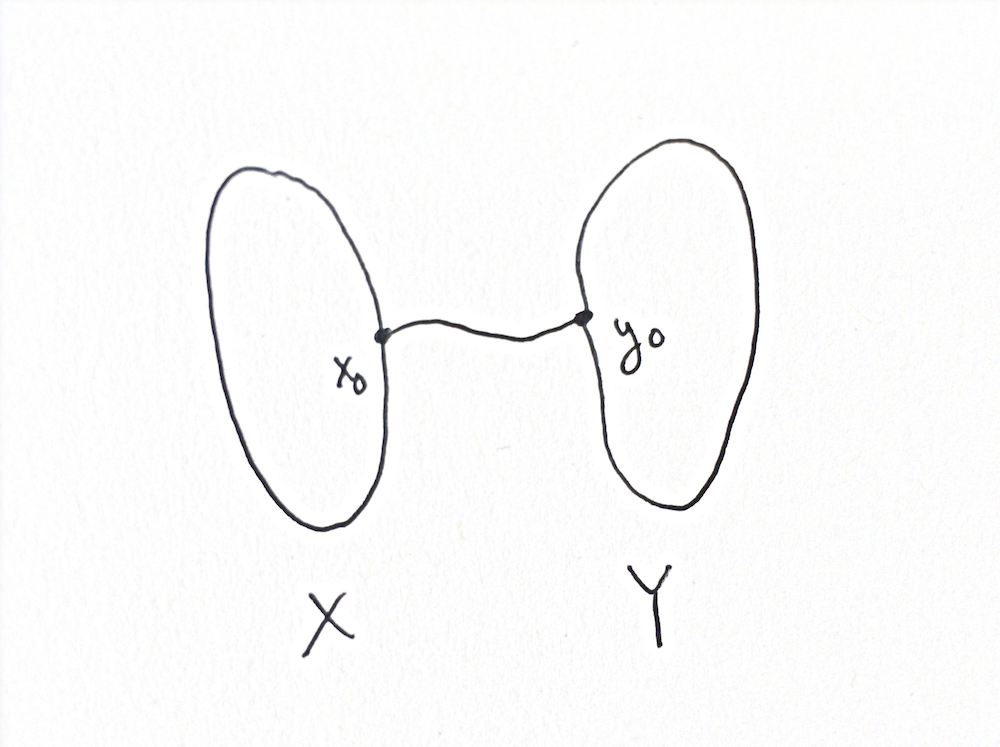
\includegraphics{pics/whisker-gluing.png}}
  \centering
\end{figure}




\begin{example} As another example, suppose $\ast \hookto X$ is the inclusion of a point $x\in X$. Taking the cofiber of this map\footnote{Recall the cofiber of a map $f: X \to Y$ is the colimit $\colim \left( \ast \from X \xto{f} Y \right)$.} is the same as simply gluing the point $\ast$ to $x\in X$, and you simply end up with the space $X$. If, instead, you wanted to take the \textit{homotopy cofiber} of this map, you would end up with the space $X$, with a small whisker protruding from the point $x$, ending at the point $\ast$. This procedure has a name, and it is actually called \textit{whiskering}. For example if $(X,x)$ is a based space which is not well based\footnote{Recall a space is \textit{well-based/non-degenerately based} if the inclusion of the basepoint is a cofibraion.}, we can take the based space $(\hocolim(\ast \hookto X),\ast)$, which becomes well-based.
\end{example}

\begin{figure}[H]
  \scalebox{0.2}{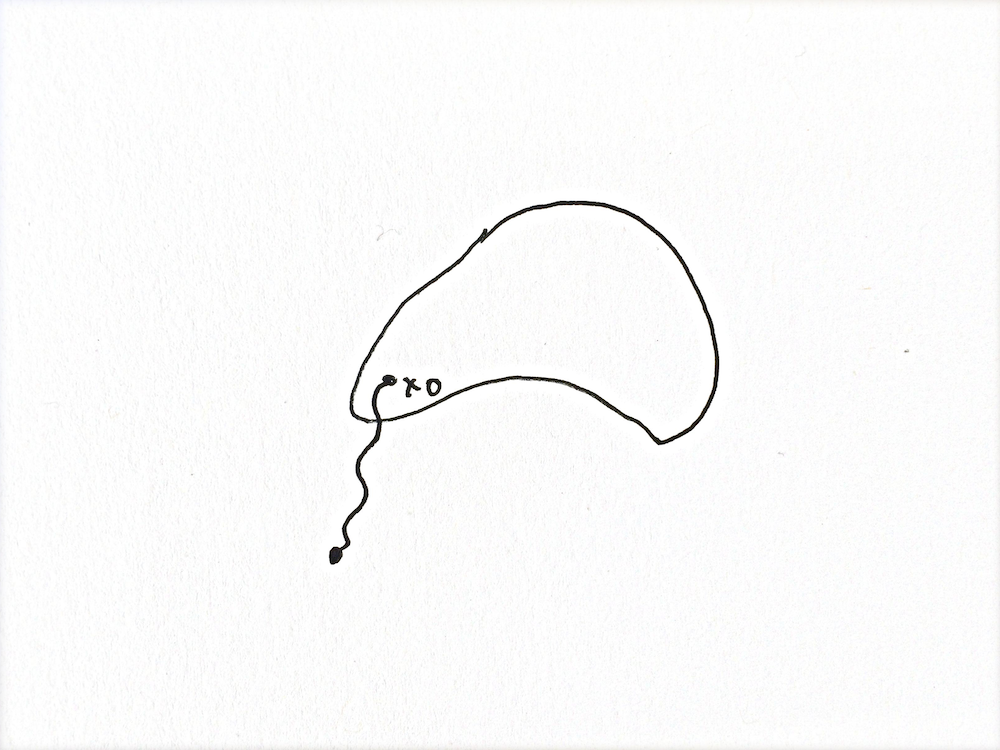
\includegraphics{pics/whisker.png}}
  \centering
\end{figure}



\begin{example} Consider the map $S^1 \to \ast$ collapsing the sphere to a point. The cofiber of this map is $\ast$, that is, a one-point space. However to form the homotopy cofiber, we must draw a path from each point on $S^1$ to the point $\ast$. Here is where we sweep some more rigor under the rug, and illustrate what we mean by ``in a continuous fashion'' in our characterization of homotopy colimits. When creating our paths from points on $S^1$ to $\ast$, a small change in the choice of point on the circle $S^1$ should correspond to a small change in the path drawn. We shouldn't think of these paths as a loose collection of uncountably many strings, flying everywhere and connecting each point on $S^1$ to $\ast$. Instead, nearby strings should coagulate to form surfaces.

\begin{figure}[H]
  \scalebox{0.2}{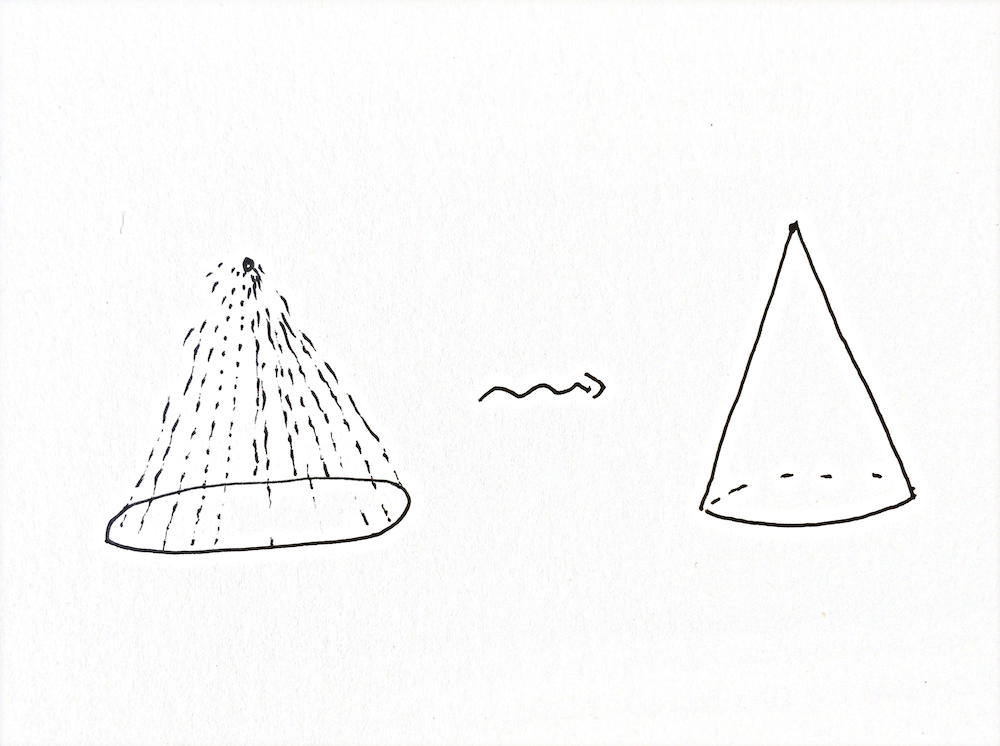
\includegraphics{pics/cone.png}}
  \centering
\end{figure}

If you've followed this rough description, then it would make sense to you that the homotopy cofiber of the map $S^1 \to \ast$ becomes a hollow cone over $S^1$, whose vertex is the point $\ast$. If, on the other hand, this lack of rigor has disgusted you, then the authors understand wholeheartedly and invite you to read \cite{Dugger}.
\end{example}


In the previous examples, the resulting space obtained by taking a homotopy colimit was weakly homotopy equivalent to the original one obtained by taking a colimit. We can ask whether this will always be the case, which the following example (a rephrased version of Example 2.1 in \cite{Dugger}) illustrates.


\begin{example} Consider the diagram $\ast \from S^1 \to \ast$. Its colimit is the pushout $\ast \amalg_{S^1} \ast \cong \ast$, which is just a one-point space. On the other hand, its homotopy colimit can be constructed via the previous example. By gluing $S^1$ to each point $\ast$, we obtain two hollow cones which are identified together along their bases. That is, we obtain a 2-sphere $S^2$. Note that $S^2 \not \simeq \ast$!
\end{example}

This is an example of a general phenomena; for a diagram $D: I \to \Top$, it is often the case that $\colim(D) \not\simeq \hocolim(D)$.


\begin{remark} In the previous section we have said that a homotopy colimit ``is'' a certain space. The reader should be advised that homotopy colimits are only defined up to weak equivalence. This turns out to be both a blessing and a curse, in that we fail to obtain a well-defined construction in the topological category, however the ambiguity allows homotopy colimits to satisfy a property that colimits fail to satisfy: \textit{homotopy invariance.} We will make this precise.
\end{remark}

\subsection{Homotopy Invariance}

\begin{definition} A \textit{weak homotopy equivalence of diagrams} is a natural transformation $D \Rightarrow D'$ (occasionally denoted $D \simeq D'$) between two diagrams $D,D' : I \to \Top$ whose components are weak homotopy equivalences.
\end{definition}

\begin{example}\label{ex:we-of-diagrams} Let our index category be $I = \bullet \from \bullet \to \bullet$, and let $D(I) = \left(D^{n+1} \hookfrom S^n \hookto D^{n+1}\right)$, and $D'(I) = \left(\ast \from S^n \to \ast \right)$. Then there is a weak homotopy equivalence of diagrams $D \Rightarrow D'$ whose components are the identity map on $S^n$ and the contraction $D^{n+1} \xto{\sim} \ast$ on the disks.
\end{example}

\begin{remark} Colimits fail to satisfy \textit{homotopy invariance}. That is, for a weak homotopy equivalence of diagrams $D\simeq D'$, we may have that $\colim(D) \not\simeq \colim(D')$.
\end{remark}

\begin{exercise} See in Example \ref{ex:we-of-diagrams} that $\colim(D) = S^{n+1}$ but $\colim(D') = \ast$.
\end{exercise}

\begin{theorem} Homotopy colimits satisfy homotopy invariance. That is, for $D\simeq D'$, one always has that
\begin{align*}
    \hocolim(D) \simeq \hocolim(D').
\end{align*}
\end{theorem}

\begin{corollary} Given any diagram, we may replace maps and objects in the diagram by weakly equivalent ones and obtain the same homotopy colimit.
\end{corollary}


\subsection{Homotopy colimits coinciding with colimits}

There are many deep questions to ask about homotopy colimits, but perhaps the first one that we might be curious about is when homotopy colimits and colimits coincide. This question is non-trivial to answer, and as always we defer to \cite{Dugger} for a full treatment. However we will give one example, which is a stronger condition on a diagram than one needs in general, but will suit our examples:

\begin{proposition} If a diagram $D: I \to \Top$ has the property that all of its maps are cofibrations, then $\colim(D) \simeq \hocolim(D)$.
\end{proposition}

In particular, if the maps are inclusions of subspaces which form a relative CW complex, they are cofibrations.

This fact, combined with homotopy invariance of homotopy colimits, will allow us to provide a characterization of a lot of phenomena occurring in algebraic topology in terms of homotopy colimits.

\begin{example} We have that $\Sigma X = \hocolim(\ast \from X \to \ast)$.
\end{example}
\begin{proof} Let $CX$ denote the cone over $X$, and note that $CX \simeq \ast$ is contractible. Then since the inclusion $X \hookto CX$ is a relative CW complex, one has
\begin{align*}
    \Sigma X &= \colim \left( \begin{tikzcd}[ampersand replacement=\&] X\rar[hook]\dar[hook] \& CX \\ CX \& \end{tikzcd} \right) = \hocolim \left( \begin{tikzcd}[ampersand replacement=\&] X\rar[hook]\dar[hook] \& CX \\ CX \& \end{tikzcd} \right) \\
    &=\hocolim \left( \begin{tikzcd}[ampersand replacement=\&] X\rar[hook]\dar[hook] \& \ast \\ \ast \& \end{tikzcd} \right).
\end{align*}
\end{proof}

\begin{example} Let $\phi: S^n \to X_n$ be the attaching map for an $(n+1)$-cell, and let $X_{n+1}$ be the space obtained by attaching this cell. Then
\begin{align*}
    X_{n+1} = \hocofib\left(S^n \xto{\phi} X_n\right).
\end{align*}
\end{example}
\begin{proof} Again we apply the previous proposition and homotopy invariance of homotopy colimits. We have that
\begin{align*}
    X_{n+1} &= \colim \left( \begin{tikzcd}[ampersand replacement=\&] S^n\rar[hook,"\phi" above]\dar[hook] \& X_n \\ D^{n+1} \& \end{tikzcd} \right) = \hocolim \left( \begin{tikzcd}[ampersand replacement=\&] S^n\rar[hook,"\phi" above]\dar[hook] \& X_n \\ D^{n+1} \& \end{tikzcd} \right) \\
    &=\hocolim \left( \begin{tikzcd}[ampersand replacement=\&] S^n\rar[hook,"\phi" above]\dar[hook] \& X_n \\ \ast \& \end{tikzcd} \right) = \hocofib(\phi).
\end{align*}
\end{proof}

\begin{example} For a map $f: X\to Y$, the \textit{mapping cylinder}, defined on \cite[p.2]{hatcher} may be thought of as $M_f = \hocolim(X \xto{f} Y)$.
\end{example}


\begin{example} For a map $f: X\to Y$ \textit{mapping cone} $C_f$, defined on \cite[p.13]{hatcher}, is the homotopy cofiber of the map $f$:
\begin{align*}
    C_f = \hocofib(f).
\end{align*}
\end{example}

\begin{example} The \textit{join} of two spaces $X$ and $Y$, defined on \cite[p.9]{hatcher}, is the homotopy pushout $\hocolim(X \from X\times Y \to Y)$.
\end{example}

\begin{example} As a generalization of the previous example, the \textit{double mapping cylinder}, defined on \cite[p.80]{may}, is the homotopy pushout $\hocolim( A \from X \to B)$.
\end{example}

\begin{example} The \textit{mapping telescope}, defined on \cite[p.138]{hatcher}, is the homotopy colimit
\begin{align*}
    \hocolim\left(X_0 \xto{f_0} X_1 \xto{f_1} \cdots \right).
\end{align*}

\end{example}




\begin{theorem} \cite[Theorem~24.9]{chacholski} Homotopy colimits commute.
\end{theorem}

\begin{corollary} On \cite[p.57]{may}, a critical aspect of the cofiber sequence generated by a map $f$ is that there is a weak equivalence (really a homeomorphism) $\Sigma C_f \simeq C(\Sigma f)$. This can be easily remembered by the fact that homotopy colimits commute.
\end{corollary}







%%%%%%%%%%






%\printbibliography

\bibliographystyle{amsalpha}
\bibliography{619.bib}







%%
%	Index
%%
\newpage
\printindex[ind]



\end{document}
